%&preformat-disser
\RequirePackage[l2tabu,orthodox]{nag} % Раскомментировав, можно в логе получать рекомендации относительно правильного использования пакетов и предупреждения об устаревших и нерекомендуемых пакетах
% Формат А4, 14pt (ГОСТ Р 7.0.11-2011, 5.3.6)
\documentclass[a4paper,14pt,oneside,openany]{memoir}

\input{common/setup}            % общие настройки шаблона
%%% Проверка используемого TeX-движка %%%
\RequirePackage{ifxetex, ifluatex}
\newif\ifxetexorluatex   % определяем новый условный оператор (http://tex.stackexchange.com/a/47579)
\ifxetex
    \xetexorluatextrue
\else
    \ifluatex
        \xetexorluatextrue
    \else
        \xetexorluatexfalse
    \fi
\fi

\newif\ifsynopsis           % Условие, проверяющее, что документ --- автореферат

\RequirePackage{etoolbox}[2015/08/02]               % Для продвинутой проверки разных условий
\providebool{presentation}

%%% Поля и разметка страницы %%%
\usepackage{pdflscape}                              % Для включения альбомных страниц
\usepackage{geometry}                               % Для последующего задания полей

%%% Математические пакеты %%%
\usepackage{amsthm,amsmath,amscd}   % Математические дополнения от AMS
\usepackage{amsfonts,amssymb}       % Математические дополнения от AMS
\usepackage{mathtools}              % Добавляет окружение multlined

%%%% Установки для размера шрифта 14 pt %%%%
%% Формирование переменных и констант для сравнения (один раз для всех подключаемых файлов)%%
%% должно располагаться до вызова пакета fontspec или polyglossia, потому что они сбивают его работу
\newlength{\curtextsize}
\newlength{\bigtextsize}
\setlength{\bigtextsize}{13.9pt}

\makeatletter
%\show\f@size                                       % неплохо для отслеживания, но вызывает стопорение процесса, если документ компилируется без команды  -interaction=nonstopmode
\setlength{\curtextsize}{\f@size pt}
\makeatother

%%% Кодировки и шрифты %%%
\ifxetexorluatex
    \usepackage{polyglossia}[2014/05/21]            % Поддержка многоязычности (fontspec подгружается автоматически)
\else
   %%% Решение проблемы копирования текста в буфер кракозябрами
    \ifnumequal{\value{usealtfont}}{0}{}{
        \input glyphtounicode.tex
        \input glyphtounicode-cmr.tex %from pdfx package
        \pdfgentounicode=1
    }
    \usepackage{cmap}                               % Улучшенный поиск русских слов в полученном pdf-файле
    \ifnumequal{\value{usealtfont}}{2}{}{
        \defaulthyphenchar=127                      % Если стоит до fontenc, то переносы не впишутся в выделяемый текст при копировании его в буфер обмена
    }
    \usepackage{textcomp}
    \usepackage[T1,T2A]{fontenc}                    % Поддержка русских букв
    \ifnumequal{\value{usealtfont}}{1}{% Используется pscyr, при наличии
        \IfFileExists{pscyr.sty}{\usepackage{pscyr}}{}  % Подключение pscyr
    }{}
    \usepackage[utf8]{inputenc}[2014/04/30]         % Кодировка utf8
    \usepackage[english, main=russian]{babel}[2014/03/24]% Языки: русский, английский
    \ifnumequal{\value{usealtfont}}{2}{
        % http://dxdy.ru/post1238763.html#p1238763
        \usepackage[scaled=0.960]{XCharter}[2017/12/19] % Подключение русифицированных шрифтов XCharter
        \usepackage[charter, vvarbb, scaled=1.048]{newtxmath}[2017/12/14]
        \setDisplayskipStretch{-0.078}
    }{}
\fi

%%% Оформление абзацев %%%
\usepackage{indentfirst}                            % Красная строка

%%% Цвета %%%
\ifpresentation
\else
    \usepackage[dvipsnames, table, hyperref]{xcolor} % Совместимо с tikz
\fi

%%% Таблицы %%%
\usepackage{longtable,ltcaption}                    % Длинные таблицы
\usepackage{multirow,makecell}                      % Улучшенное форматирование таблиц

%%% Общее форматирование
\usepackage{soulutf8}                               % Поддержка переносоустойчивых подчёркиваний и зачёркиваний
\usepackage{icomma}                                 % Запятая в десятичных дробях

%%% Оптимизация расстановки переносов и длины последней строки абзаца
\ifluatex
    \ifnumequal{\value{draft}}{1}{% Черновик
        \usepackage[hyphenation, lastparline, nosingleletter, homeoarchy,
        rivers, draft]{impnattypo}
    }{% Чистовик
        \usepackage[hyphenation, lastparline, nosingleletter]{impnattypo}
    }
\else
    \usepackage[hyphenation, lastparline]{impnattypo}
\fi

%%% Гиперссылки %%%
\usepackage{hyperref}[2012/11/06]

%%% Изображения %%%
\usepackage{graphicx}[2014/04/25]                   % Подключаем пакет работы с графикой

%%% Счётчики %%%
\usepackage[figure,table]{totalcount}               % Счётчик рисунков и таблиц
\usepackage{totcount}                               % Пакет создания счётчиков на основе последнего номера подсчитываемого элемента (может требовать дважды компилировать документ)
\usepackage{totpages}                               % Счётчик страниц, совместимый с hyperref (ссылается на номер последней страницы). Желательно ставить последним пакетом в преамбуле

%%% Продвинутое управление групповыми ссылками (пока только формулами) %%%
\ifpresentation
\else
    \ifxetexorluatex
        \usepackage{cleveref}                           % cleveref корректно считывает язык из настроек polyglossia
    \else
        \usepackage[russian]{cleveref}                  % cleveref имеет сложности со считыванием языка из babel. Такое решение русификации вывода выбрано вместо определения в documentclass из опасности что-то лишнее передать во все остальные пакеты, включая библиографию.
    \fi
    \creflabelformat{equation}{#2#1#3}                  % Формат по умолчанию ставил круглые скобки вокруг каждого номера ссылки, теперь просто номера ссылок без какого-либо дополнительного оформления
    \crefrangelabelformat{equation}{#3#1#4\cyrdash#5#2#6}   % Интервалы в русском языке принято делать через тире, если иное не оговорено
\fi


\ifnumequal{\value{draft}}{1}{% Черновик
    \usepackage[firstpage]{draftwatermark}
    \SetWatermarkText{DRAFT}
    \SetWatermarkFontSize{14pt}
    \SetWatermarkScale{15}
    \SetWatermarkAngle{45}
}{}

%%% Исправление положения якорей подписей (под)рисунков %%%
% Без hypcap и патча, при клике по ссылке на подрисунок, просмотрщик pdf прыгает "к подписи" а не "к рисунку".
% Подробнее: https://github.com/AndreyAkinshin/Russian-Phd-LaTeX-Dissertation-Template/issues/238
% (!) Даже с патчем, если мешать в одной фиге разные типы подфиг (subbottom и subcaption) - ссылки всё равно будут работать неправильно  (см. https://www.overleaf.com/read/czmbmmtnqrrg ).
\ifpresentation
\else
	\usepackage[all]{hypcap}
	
	\makeatletter
	\ltx@ifclasslater{memoir}{2018/12/13}{
		% Предполагается, что в следующей версии класс будет исправлен
		\typeout{Assuming this version of memoir is free from the jumping-to-caption bug.}
	}{		
		\RequirePackage{xpatch}		
		
		\newcommand\mem@step@subcounter{%
		  \refstepcounter{sub\@captype}\@contkeep%
		}
		
		\xpatchcmd{\@memsubbody}%
		{\refstepcounter{sub\@captype}\@contkeep}% search pattern
		{}% replacement
		{\typeout{@memsubbody is patched}}%
		{\typeout{@memsubbody is NOT patched}}%
		
		\xpatchcmd{\@memcontsubbody}%
		{\refstepcounter{sub\@captype}\@contkeep}% pattern
		{}% replacement
		{\typeout{@memcontsubbody is patched}}%
		{\typeout{@memcontsubbody is NOT patched}}%
		
		\xpatchcmd{\@memsubfloat}%
		{\vtop\bgroup}% search pattern
		{\vtop\bgroup\mem@step@subcounter}% replacement
		{\typeout{@memsubfloat patch is ok}}%
		{\typeout{@memsubfloat patch is NOT ok}}%
		
		
		\xpatchcmd{\subcaption}%
		{\refstepcounter{sub\@captype}}% search pattern
		{\H@refstepcounter{sub\@captype}}% replacement
		{\typeout{subcaption second patch is ok}}%
		{\typeout{subcaption second patch is NOT ok}}%			
	}
	\makeatother
\fi

\usepackage{longtable}
%%% Цитата, не приводимая в автореферате:
% возможно, актуальна только для biblatex
%\newcommand{\citeinsynopsis}[1]{\ifsynopsis\else ~\cite{#1} \fi}

\usepackage{subfig}
\usepackage{subcaption}         % Пакеты общие для диссертации и автореферата
\synopsisfalse                      % Этот документ --- не автореферат
\input{Dissertation/dispackages}    % Пакеты для диссертации
\input{Dissertation/userpackages}   % Пакеты для специфических пользовательских задач

\input{Dissertation/setup}      % Упрощённые настройки шаблона

% Новые переменные, которые могут использоваться во всём проекте
% ГОСТ 7.0.11-2011
% 9.2 Оформление текста автореферата диссертации
% 9.2.1 Общая характеристика работы включает в себя следующие основные структурные
% элементы:
% актуальность темы исследования;
\newcommand{\actualityTXT}{Актуальность темы.}
% степень ее разработанности;
\newcommand{\progressTXT}{Степень разработанности темы.}
% цели и задачи;
\newcommand{\aimTXT}{Целью}
\newcommand{\tasksTXT}{задачи}
% научную новизну;
\newcommand{\noveltyTXT}{Научная новизна}
% теоретическую и практическую значимость работы;
%\newcommand{\influenceTXT}{Теоретическая и практическая значимость}
% или чаще используют просто
\newcommand{\influenceTXT}{Практическая значимость}
% методологию и методы исследования;
\newcommand{\methodsTXT}{Методология и методы исследования.}
% положения, выносимые на защиту;
\newcommand{\defpositionsTXT}{Основные положения, выносимые на~защиту:}
% степень достоверности и апробацию результатов.
\newcommand{\reliabilityTXT}{Достоверность}
\newcommand{\probationTXT}{Апробация работы.}

\newcommand{\contributionTXT}{Личный вклад.}
\newcommand{\publicationsTXT}{Публикации.}


\newcommand{\authorbibtitle}{Публикации автора по теме диссертации}
\newcommand{\vakbibtitle}{В изданиях из списка ВАК РФ}
\newcommand{\notvakbibtitle}{В прочих изданиях}
\newcommand{\confbibtitle}{В сборниках трудов конференций}
\newcommand{\fullbibtitle}{Список литературы} % (ГОСТ Р 7.0.11-2011, 4)
         % Новые переменные, для всего проекта

%%% Основные сведения %%%
\newcommand{\thesisAuthorLastName}{Бурдинов}
\newcommand{\thesisAuthorOtherNames}{Константин Алексеевич}
\newcommand{\thesisAuthorInitials}{К.\,А.}
\newcommand{\thesisAuthor}             % Диссертация, ФИО автора
{%
    \texorpdfstring{% \texorpdfstring takes two arguments and uses the first for (La)TeX and the second for pdf
        \thesisAuthorLastName~\thesisAuthorOtherNames% так будет отображаться на титульном листе или в тексте, где будет использоваться переменная
    }{%
        \thesisAuthorLastName, \thesisAuthorOtherNames% эта запись для свойств pdf-файла. В таком виде, если pdf будет обработан программами для сбора библиографических сведений, будет правильно представлена фамилия.
    }
}
\newcommand{\thesisAuthorShort}        % Диссертация, ФИО автора инициалами
{\thesisAuthorInitials~\thesisAuthorLastName}
%\newcommand{\thesisUdk}                % Диссертация, УДК
%{\todo{xxx.xxx}}
\newcommand{\thesisTitle}              % Диссертация, название
{СИНТЕЗ, МОДЕЛИРОВАНИЕ И ИСПЫТАНИЕ СИСТЕМ УПРАВЛЕНИЯ БОРТОВЫМ ОПТИКО-ЭЛЕКТРОННЫМ ПРИБОРОМ ВИЗИРОВАНИЯ И ПРОТИВОДЕЙСТВИЯ}
\newcommand{\thesisSpecialtyNumber}    % Диссертация, специальность, номер
{05.11.07}
\newcommand{\thesisSpecialtyTitle}     % Диссертация, специальность, название (название взято с сайта ВАК для примера)
{Оптические и оптико-электронные приборы и комплексы}
%% \newcommand{\thesisSpecialtyTwoNumber} % Диссертация, вторая специальность, номер
%% {\todo{XX.XX.XX}}
%% \newcommand{\thesisSpecialtyTwoTitle}  % Диссертация, вторая специальность, название
%% {\todo{Теория и~методика физического воспитания, спортивной тренировки,
%% оздоровительной и~адаптивной физической культуры}}
\newcommand{\thesisDegree}             % Диссертация, ученая степень
{кандидата технических наук}
\newcommand{\thesisDegreeShort}        % Диссертация, ученая степень, краткая запись
{канд. тех. наук}
\newcommand{\thesisCity}               % Диссертация, город написания диссертации
{Казань}
\newcommand{\thesisYear}               % Диссертация, год написания диссертации
{2020}
\newcommand{\thesisOrganization}       % Диссертация, организация
{ФЕДЕРАЛЬНОЕ ГОСУДАРСТВЕННОЕ БЮДЖЕТНОЕ ОБРАЗОВАТЕЛЬНОЕ УЧРЕЖДЕНИЕ ВЫСШЕГО ПРОФФЕСИОНАЛЬНОГО ОБРАЗОВАНИЯ <<КАЗАНСКИЙ НАЦИОНАЛЬНЫЙ ИССЛЕДОВАТЕЛЬСКИЙ ТЕХНИЧЕСКИЙ УНИВЕРСИТЕТ ИМ. А.Н. ТУПОЛЕВА-КАИ>>}
\newcommand{\thesisOrganizationShort}  % Диссертация, краткое название организации для доклада
{КНИТУ-КАИ}

\newcommand{\thesisInOrganization}     % Диссертация, организация в предложном падеже: Работа выполнена в ...
{\todo{учреждении с~длинным длинным длинным длинным названием, в~котором
выполнялась данная диссертационная работа}}

%% \newcommand{\supervisorDead}{}           % Рисовать рамку вокруг фамилии
\newcommand{\supervisorFio}              % Научный руководитель, ФИО
{Карпов Алексей Иванович}
\newcommand{\supervisorRegalia}          % Научный руководитель, регалии
{кандидат технических наук, доцент}
\newcommand{\supervisorFioShort}         % Научный руководитель, ФИО
{А.\,И.~Карпов}
\newcommand{\supervisorRegaliaShort}     % Научный руководитель, регалии
{к.т.н.,~доцент}

%% \newcommand{\supervisorTwoDead}{}        % Рисовать рамку вокруг фамилии
%% \newcommand{\supervisorTwoFio}           % Второй научный руководитель, ФИО
%% {\todo{Фамилия Имя Отчество}}
%% \newcommand{\supervisorTwoRegalia}       % Второй научный руководитель, регалии
%% {\todo{уч. степень, уч. звание}}
%% \newcommand{\supervisorTwoFioShort}      % Второй научный руководитель, ФИО
%% {\todo{И.\,О.~Фамилия}}
%% \newcommand{\supervisorTwoRegaliaShort}  % Второй научный руководитель, регалии
%% {\todo{уч.~ст.,~уч.~зв.}}

\newcommand{\opponentOneFio}           % Оппонент 1, ФИО
{\todo{Фамилия Имя Отчество}}
\newcommand{\opponentOneRegalia}       % Оппонент 1, регалии
{\todo{доктор физико-математических наук, профессор}}
\newcommand{\opponentOneJobPlace}      % Оппонент 1, место работы
{\todo{Не очень длинное название для места работы}}
\newcommand{\opponentOneJobPost}       % Оппонент 1, должность
{\todo{старший научный сотрудник}}

\newcommand{\opponentTwoFio}           % Оппонент 2, ФИО
{\todo{Фамилия Имя Отчество}}
\newcommand{\opponentTwoRegalia}       % Оппонент 2, регалии
{\todo{кандидат физико-математических наук}}
\newcommand{\opponentTwoJobPlace}      % Оппонент 2, место работы
{\todo{Основное место работы c длинным длинным длинным длинным названием}}
\newcommand{\opponentTwoJobPost}       % Оппонент 2, должность
{\todo{старший научный сотрудник}}

%% \newcommand{\opponentThreeFio}         % Оппонент 3, ФИО
%% {\todo{Фамилия Имя Отчество}}
%% \newcommand{\opponentThreeRegalia}     % Оппонент 3, регалии
%% {\todo{кандидат физико-математических наук}}
%% \newcommand{\opponentThreeJobPlace}    % Оппонент 3, место работы
%% {\todo{Основное место работы c длинным длинным длинным длинным названием}}
%% \newcommand{\opponentThreeJobPost}     % Оппонент 3, должность
%% {\todo{старший научный сотрудник}}

\newcommand{\leadingOrganizationTitle} % Ведущая организация, дополнительные строки. Удалить, чтобы не отображать в автореферате
{\todo{Федеральное государственное бюджетное образовательное учреждение высшего
профессионального образования с~длинным длинным длинным длинным названием}}

\newcommand{\defenseDate}              % Защита, дата
{\todo{DD mmmmmmmm YYYY~г.~в~XX часов}}
\newcommand{\defenseCouncilNumber}     % Защита, номер диссертационного совета
{\todo{Д\,123.456.78}}
\newcommand{\defenseCouncilTitle}      % Защита, учреждение диссертационного совета
{\todo{Название учреждения}}
\newcommand{\defenseCouncilAddress}    % Защита, адрес учреждение диссертационного совета
{\todo{Адрес}}
\newcommand{\defenseCouncilPhone}      % Телефон для справок
{\todo{+7~(0000)~00-00-00}}

\newcommand{\defenseSecretaryFio}      % Секретарь диссертационного совета, ФИО
{\todo{Фамилия Имя Отчество}}
\newcommand{\defenseSecretaryRegalia}  % Секретарь диссертационного совета, регалии
{\todo{д-р~физ.-мат. наук}}            % Для сокращений есть ГОСТы, например: ГОСТ Р 7.0.12-2011 + http://base.garant.ru/179724/#block_30000

\newcommand{\synopsisLibrary}          % Автореферат, название библиотеки
{\todo{Название библиотеки}}
\newcommand{\synopsisDate}             % Автореферат, дата рассылки
{\todo{DD mmmmmmmm YYYY года}}

% To avoid conflict with beamer class use \providecommand
\providecommand{\keywords}%            % Ключевые слова для метаданных PDF диссертации и автореферата
{}
             % Основные сведения
\input{common/fonts}            % Определение шрифтов (частичное)
%%% Шаблон %%%
\DeclareRobustCommand{\todo}{\textcolor{red}}       % решаем проблему превращения названия цвета в результате \MakeUppercase, http://tex.stackexchange.com/a/187930, \DeclareRobustCommand protects \todo from expanding inside \MakeUppercase
\AtBeginDocument{%
    \setlength{\parindent}{2.5em}                   % Абзацный отступ. Должен быть одинаковым по всему тексту и равен пяти знакам (ГОСТ Р 7.0.11-2011, 5.3.7).
}

%%% Подписи %%%
\setlength{\abovecaptionskip}{0pt}   % Отбивка над подписью
\setlength{\belowcaptionskip}{0pt}   % Отбивка под подписью
%\captionwidth{\linewidth}
\normalcaptionwidth

%%% Таблицы %%%
\ifnumequal{\value{tabcap}}{0}{%
    \newcommand{\tabcapalign}{\raggedright}  % по левому краю страницы или аналога parbox
    \renewcommand{\tablabelsep}{~\cyrdash\ } % тире как разделитель идентификатора с номером от наименования
    \newcommand{\tabtitalign}{}
}{%
    \ifnumequal{\value{tablaba}}{0}{%
        \newcommand{\tabcapalign}{\raggedright}  % по левому краю страницы или аналога parbox
    }{}

    \ifnumequal{\value{tablaba}}{1}{%
        \newcommand{\tabcapalign}{\centering}    % по центру страницы или аналога parbox
    }{}

    \ifnumequal{\value{tablaba}}{2}{%
        \newcommand{\tabcapalign}{\raggedleft}   % по правому краю страницы или аналога parbox
    }{}

    \ifnumequal{\value{tabtita}}{0}{%
        \newcommand{\tabtitalign}{\par\raggedright}  % по левому краю страницы или аналога parbox
    }{}

    \ifnumequal{\value{tabtita}}{1}{%
        \newcommand{\tabtitalign}{\par\centering}    % по центру страницы или аналога parbox
    }{}

    \ifnumequal{\value{tabtita}}{2}{%
        \newcommand{\tabtitalign}{\par\raggedleft}   % по правому краю страницы или аналога parbox
    }{}
}

\precaption{\tabcapalign} % всегда идет перед подписью или \legend
\captionnamefont{\normalfont\normalsize} % Шрифт надписи «Таблица #»; также определяет шрифт у \legend
\captiondelim{\tablabelsep} % разделитель идентификатора с номером от наименования
\captionstyle[\tabtitalign]{\tabtitalign}
\captiontitlefont{\normalfont\normalsize} % Шрифт с текстом подписи

%%% Рисунки %%%
\setfloatadjustment{figure}{%
    \setlength{\abovecaptionskip}{0pt}   % Отбивка над подписью
    \setlength{\belowcaptionskip}{0pt}   % Отбивка под подписью
    \precaption{} % всегда идет перед подписью или \legend
    \captionnamefont{\normalfont\normalsize} % Шрифт надписи «Рисунок #»; также определяет шрифт у \legend
    \captiondelim{\figlabelsep} % разделитель идентификатора с номером от наименования
    \captionstyle[\centering]{\centering} % Центрирование подписей, заданных командой \caption и \legend
    \captiontitlefont{\normalfont\normalsize} % Шрифт с текстом подписи
    \postcaption{} % всегда идет после подписи или \legend, и с новой строки
}

%%% Подписи подрисунков %%%
\newsubfloat{figure} % Включает возможность использовать подрисунки у окружений figure
\renewcommand{\thesubfigure}{\asbuk{subfigure}}           % Буквенные номера подрисунков
\subcaptionsize{\normalsize} % Шрифт подписи названий подрисунков (не отличается от основного)
\subcaptionlabelfont{\normalfont}
\subcaptionfont{\!\!) \normalfont} % Вот так тут добавили скобку после буквы.
\subcaptionstyle{\centering}
%\subcaptionsize{\fontsize{12pt}{13pt}\selectfont} % объявляем шрифт 12pt для использования в подписях, тут же надо интерлиньяж объявлять, если не наследуется

%%% Настройки гиперссылок %%%
\ifluatex
    \hypersetup{
        unicode,                % Unicode encoded PDF strings
    }
\fi

\hypersetup{
    linktocpage=true,           % ссылки с номера страницы в оглавлении, списке таблиц и списке рисунков
%    linktoc=all,                % both the section and page part are links
%    pdfpagelabels=false,        % set PDF page labels (true|false)
    plainpages=false,           % Forces page anchors to be named by the Arabic form  of the page number, rather than the formatted form
    colorlinks,                 % ссылки отображаются раскрашенным текстом, а не раскрашенным прямоугольником, вокруг текста
    linkcolor={linkcolor},      % цвет ссылок типа ref, eqref и подобных
    citecolor={citecolor},      % цвет ссылок-цитат
    urlcolor={urlcolor},        % цвет гиперссылок
%    hidelinks,                  % Hide links (removing color and border)
    pdftitle={\thesisTitle},    % Заголовок
    pdfauthor={\thesisAuthor},  % Автор
    pdfsubject={\thesisSpecialtyNumber\ \thesisSpecialtyTitle},      % Тема
%    pdfcreator={Создатель},     % Создатель, Приложение
%    pdfproducer={Производитель},% Производитель, Производитель PDF
    pdfkeywords={\keywords},    % Ключевые слова
    pdflang={ru},
}
\ifnumequal{\value{draft}}{1}{% Черновик
    \hypersetup{
        draft,
    }
}{}

%%% Списки %%%
% Используем короткое тире (endash) для ненумерованных списков (ГОСТ 2.105-95, пункт 4.1.7, требует дефиса, но так лучше смотрится)
\renewcommand{\labelitemi}{\normalfont\bfseries{--}}

% Перечисление строчными буквами латинского алфавита (ГОСТ 2.105-95, 4.1.7)
%\renewcommand{\theenumi}{\alph{enumi}}
%\renewcommand{\labelenumi}{\theenumi)}

% Перечисление строчными буквами русского алфавита (ГОСТ 2.105-95, 4.1.7)
\makeatletter
\AddEnumerateCounter{\asbuk}{\russian@alph}{щ}      % Управляем списками/перечислениями через пакет enumitem, а он 'не знает' про asbuk, потому 'учим' его
\makeatother
%\renewcommand{\theenumi}{\asbuk{enumi}} %первый уровень нумерации
%\renewcommand{\labelenumi}{\theenumi)} %первый уровень нумерации
\renewcommand{\theenumii}{\asbuk{enumii}} %второй уровень нумерации
\renewcommand{\labelenumii}{\theenumii)} %второй уровень нумерации
\renewcommand{\theenumiii}{\arabic{enumiii}} %третий уровень нумерации
\renewcommand{\labelenumiii}{\theenumiii)} %третий уровень нумерации

\setlist{nosep,%                                    % Единый стиль для всех списков (пакет enumitem), без дополнительных интервалов.
    labelindent=\parindent,leftmargin=*%            % Каждый пункт, подпункт и перечисление записывают с абзацного отступа (ГОСТ 2.105-95, 4.1.8)
}
           % Стили общие для диссертации и автореферата
\input{Dissertation/disstyles}  % Стили для диссертации
% для вертикального центрирования ячеек в tabulary
\def\zz{\ifx\[$\else\aftergroup\zzz\fi}
%$ \] % <-- чиним подсветку синтаксиса в некоторых редакторах
\def\zzz{\setbox0\lastbox
\dimen0\dimexpr\extrarowheight + \ht0-\dp0\relax
\setbox0\hbox{\raise-.5\dimen0\box0}%
\ht0=\dimexpr\ht0+\extrarowheight\relax
\dp0=\dimexpr\dp0+\extrarowheight\relax 
\box0
}

\lstdefinelanguage{Renhanced}%
{keywords={abbreviate,abline,abs,acos,acosh,action,add1,add,%
        aggregate,alias,Alias,alist,all,anova,any,aov,aperm,append,apply,%
        approx,approxfun,apropos,Arg,args,array,arrows,as,asin,asinh,%
        atan,atan2,atanh,attach,attr,attributes,autoload,autoloader,ave,%
        axis,backsolve,barplot,basename,besselI,besselJ,besselK,besselY,%
        beta,binomial,body,box,boxplot,break,browser,bug,builtins,bxp,by,%
        c,C,call,Call,case,cat,category,cbind,ceiling,character,char,%
        charmatch,check,chol,chol2inv,choose,chull,class,close,cm,codes,%
        coef,coefficients,co,col,colnames,colors,colours,commandArgs,%
        comment,complete,complex,conflicts,Conj,contents,contour,%
        contrasts,contr,control,helmert,contrib,convolve,cooks,coords,%
        distance,coplot,cor,cos,cosh,count,fields,cov,covratio,wt,CRAN,%
        create,crossprod,cummax,cummin,cumprod,cumsum,curve,cut,cycle,D,%
        data,dataentry,date,dbeta,dbinom,dcauchy,dchisq,de,debug,%
        debugger,Defunct,default,delay,delete,deltat,demo,de,density,%
        deparse,dependencies,Deprecated,deriv,description,detach,%
        dev2bitmap,dev,cur,deviance,off,prev,,dexp,df,dfbetas,dffits,%
        dgamma,dgeom,dget,dhyper,diag,diff,digamma,dim,dimnames,dir,%
        dirname,dlnorm,dlogis,dnbinom,dnchisq,dnorm,do,dotplot,double,%
        download,dpois,dput,drop,drop1,dsignrank,dt,dummy,dump,dunif,%
        duplicated,dweibull,dwilcox,dyn,edit,eff,effects,eigen,else,%
        emacs,end,environment,env,erase,eval,equal,evalq,example,exists,%
        exit,exp,expand,expression,External,extract,extractAIC,factor,%
        fail,family,fft,file,filled,find,fitted,fivenum,fix,floor,for,%
        For,formals,format,formatC,formula,Fortran,forwardsolve,frame,%
        frequency,ftable,ftable2table,function,gamma,Gamma,gammaCody,%
        gaussian,gc,gcinfo,gctorture,get,getenv,geterrmessage,getOption,%
        getwd,gl,glm,globalenv,gnome,GNOME,graphics,gray,grep,grey,grid,%
        gsub,hasTsp,hat,heat,help,hist,home,hsv,httpclient,I,identify,if,%
        ifelse,Im,image,\%in\%,index,influence,measures,inherits,install,%
        installed,integer,interaction,interactive,Internal,intersect,%
        inverse,invisible,IQR,is,jitter,kappa,kronecker,labels,lapply,%
        layout,lbeta,lchoose,lcm,legend,length,levels,lgamma,library,%
        licence,license,lines,list,lm,load,local,locator,log,log10,log1p,%
        log2,logical,loglin,lower,lowess,ls,lsfit,lsf,ls,machine,Machine,%
        mad,mahalanobis,make,link,margin,match,Math,matlines,mat,matplot,%
        matpoints,matrix,max,mean,median,memory,menu,merge,methods,min,%
        missing,Mod,mode,model,response,mosaicplot,mtext,mvfft,na,nan,%
        names,omit,nargs,nchar,ncol,NCOL,new,next,NextMethod,nextn,%
        nlevels,nlm,noquote,NotYetImplemented,NotYetUsed,nrow,NROW,null,%
        numeric,\%o\%,objects,offset,old,on,Ops,optim,optimise,optimize,%
        options,or,order,ordered,outer,package,packages,page,pairlist,%
        pairs,palette,panel,par,parent,parse,paste,path,pbeta,pbinom,%
        pcauchy,pchisq,pentagamma,persp,pexp,pf,pgamma,pgeom,phyper,pico,%
        pictex,piechart,Platform,plnorm,plogis,plot,pmatch,pmax,pmin,%
        pnbinom,pnchisq,pnorm,points,poisson,poly,polygon,polyroot,pos,%
        postscript,power,ppoints,ppois,predict,preplot,pretty,Primitive,%
        print,prmatrix,proc,prod,profile,proj,prompt,prop,provide,%
        psignrank,ps,pt,ptukey,punif,pweibull,pwilcox,q,qbeta,qbinom,%
        qcauchy,qchisq,qexp,qf,qgamma,qgeom,qhyper,qlnorm,qlogis,qnbinom,%
        qnchisq,qnorm,qpois,qqline,qqnorm,qqplot,qr,Q,qty,qy,qsignrank,%
        qt,qtukey,quantile,quasi,quit,qunif,quote,qweibull,qwilcox,%
        rainbow,range,rank,rbeta,rbind,rbinom,rcauchy,rchisq,Re,read,csv,%
        csv2,fwf,readline,socket,real,Recall,rect,reformulate,regexpr,%
        relevel,remove,rep,repeat,replace,replications,report,require,%
        resid,residuals,restart,return,rev,rexp,rf,rgamma,rgb,rgeom,R,%
        rhyper,rle,rlnorm,rlogis,rm,rnbinom,RNGkind,rnorm,round,row,%
        rownames,rowsum,rpois,rsignrank,rstandard,rstudent,rt,rug,runif,%
        rweibull,rwilcox,sample,sapply,save,scale,scan,scan,screen,sd,se,%
        search,searchpaths,segments,seq,sequence,setdiff,setequal,set,%
        setwd,show,sign,signif,sin,single,sinh,sink,solve,sort,source,%
        spline,splinefun,split,sqrt,stars,start,stat,stem,step,stop,%
        storage,strstrheight,stripplot,strsplit,structure,strwidth,sub,%
        subset,substitute,substr,substring,sum,summary,sunflowerplot,svd,%
        sweep,switch,symbol,symbols,symnum,sys,status,system,t,table,%
        tabulate,tan,tanh,tapply,tempfile,terms,terrain,tetragamma,text,%
        time,title,topo,trace,traceback,transform,tri,trigamma,trunc,try,%
        ts,tsp,typeof,unclass,undebug,undoc,union,unique,uniroot,unix,%
        unlink,unlist,unname,untrace,update,upper,url,UseMethod,var,%
        variable,vector,Version,vi,warning,warnings,weighted,weights,%
        which,while,window,write,\%x\%,x11,X11,xedit,xemacs,xinch,xor,%
        xpdrows,xy,xyinch,yinch,zapsmall,zip},%
    otherkeywords={!,!=,~,$,*,\%,\&,\%/\%,\%*\%,\%\%,<-,<<-},%$
    alsoother={._$},%$
    sensitive,%
    morecomment=[l]\#,%
    morestring=[d]",%
    morestring=[d]'% 2001 Robert Denham
}%

%решаем проблему с кириллицей в комментариях (в pdflatex) https://tex.stackexchange.com/a/103712
\lstset{extendedchars=true,keepspaces=true,literate={Ö}{{\"O}}1
    {Ä}{{\"A}}1
    {Ü}{{\"U}}1
    {ß}{{\ss}}1
    {ü}{{\"u}}1
    {ä}{{\"a}}1
    {ö}{{\"o}}1
    {~}{{\textasciitilde}}1
    {а}{{\selectfont\char224}}1
    {б}{{\selectfont\char225}}1
    {в}{{\selectfont\char226}}1
    {г}{{\selectfont\char227}}1
    {д}{{\selectfont\char228}}1
    {е}{{\selectfont\char229}}1
    {ё}{{\"e}}1
    {ж}{{\selectfont\char230}}1
    {з}{{\selectfont\char231}}1
    {и}{{\selectfont\char232}}1
    {й}{{\selectfont\char233}}1
    {к}{{\selectfont\char234}}1
    {л}{{\selectfont\char235}}1
    {м}{{\selectfont\char236}}1
    {н}{{\selectfont\char237}}1
    {о}{{\selectfont\char238}}1
    {п}{{\selectfont\char239}}1
    {р}{{\selectfont\char240}}1
    {с}{{\selectfont\char241}}1
    {т}{{\selectfont\char242}}1
    {у}{{\selectfont\char243}}1
    {ф}{{\selectfont\char244}}1
    {х}{{\selectfont\char245}}1
    {ц}{{\selectfont\char246}}1
    {ч}{{\selectfont\char247}}1
    {ш}{{\selectfont\char248}}1
    {щ}{{\selectfont\char249}}1
    {ъ}{{\selectfont\char250}}1
    {ы}{{\selectfont\char251}}1
    {ь}{{\selectfont\char252}}1
    {э}{{\selectfont\char253}}1
    {ю}{{\selectfont\char254}}1
    {я}{{\selectfont\char255}}1
    {А}{{\selectfont\char192}}1
    {Б}{{\selectfont\char193}}1
    {В}{{\selectfont\char194}}1
    {Г}{{\selectfont\char195}}1
    {Д}{{\selectfont\char196}}1
    {Е}{{\selectfont\char197}}1
    {Ё}{{\"E}}1
    {Ж}{{\selectfont\char198}}1
    {З}{{\selectfont\char199}}1
    {И}{{\selectfont\char200}}1
    {Й}{{\selectfont\char201}}1
    {К}{{\selectfont\char202}}1
    {Л}{{\selectfont\char203}}1
    {М}{{\selectfont\char204}}1
    {Н}{{\selectfont\char205}}1
    {О}{{\selectfont\char206}}1
    {П}{{\selectfont\char207}}1
    {Р}{{\selectfont\char208}}1
    {С}{{\selectfont\char209}}1
    {Т}{{\selectfont\char210}}1
    {У}{{\selectfont\char211}}1
    {Ф}{{\selectfont\char212}}1
    {Х}{{\selectfont\char213}}1
    {Ц}{{\selectfont\char214}}1
    {Ч}{{\selectfont\char215}}1
    {Ш}{{\selectfont\char216}}1
    {Щ}{{\selectfont\char217}}1
    {Ъ}{{\selectfont\char218}}1
    {Ы}{{\selectfont\char219}}1
    {Ь}{{\selectfont\char220}}1
    {Э}{{\selectfont\char221}}1
    {Ю}{{\selectfont\char222}}1
    {Я}{{\selectfont\char223}}1
    {і}{{\selectfont\char105}}1
    {ї}{{\selectfont\char168}}1
    {є}{{\selectfont\char185}}1
    {ґ}{{\selectfont\char160}}1
    {І}{{\selectfont\char73}}1
    {Ї}{{\selectfont\char136}}1
    {Є}{{\selectfont\char153}}1
    {Ґ}{{\selectfont\char128}}1
}

% Ширина текста минус ширина надписи 999
\newlength{\twless}
\newlength{\lmarg}
\setlength{\lmarg}{\widthof{999}}   % ширина надписи 999
\setlength{\twless}{\textwidth-\lmarg}

\lstset{ %
%    language=R,                     %  Язык указать здесь, если во всех листингах преимущественно один язык, в результате часть настроек может пойти только для этого языка
    numbers=left,                   % where to put the line-numbers
    numberstyle=\fontsize{12pt}{14pt}\selectfont\color{Gray},  % the style that is used for the line-numbers
    firstnumber=1,                  % в этой и следующей строках задаётся поведение нумерации 5, 10, 15...
    stepnumber=5,                   % the step between two line-numbers. If it's 1, each line will be numbered
    numbersep=5pt,                  % how far the line-numbers are from the code
    backgroundcolor=\color{white},  % choose the background color. You must add \usepackage{color}
    showspaces=false,               % show spaces adding particular underscores
    showstringspaces=false,         % underline spaces within strings
    showtabs=false,                 % show tabs within strings adding particular underscores
    frame=leftline,                 % adds a frame of different types around the code
    rulecolor=\color{black},        % if not set, the frame-color may be changed on line-breaks within not-black text (e.g. commens (green here))
    tabsize=2,                      % sets default tabsize to 2 spaces
    captionpos=t,                   % sets the caption-position to top
    breaklines=true,                % sets automatic line breaking
    breakatwhitespace=false,        % sets if automatic breaks should only happen at whitespace
%    title=\lstname,                 % show the filename of files included with \lstinputlisting;
    % also try caption instead of title
    basicstyle=\fontsize{12pt}{14pt}\selectfont\ttfamily,% the size of the fonts that are used for the code
%    keywordstyle=\color{blue},      % keyword style
    commentstyle=\color{ForestGreen}\emph,% comment style
    stringstyle=\color{Mahogany},   % string literal style
    escapeinside={\%*}{*)},         % if you want to add a comment within your code
    morekeywords={*,...},           % if you want to add more keywords to the set
    inputencoding=utf8,             % кодировка кода
    xleftmargin={\lmarg},           % Чтобы весь код и полоска с номерами строк была смещена влево, так чтобы цифры не вылезали за пределы текста слева
} 

%http://tex.stackexchange.com/questions/26872/smaller-frame-with-listings
% Окружение, чтобы листинг был компактнее обведен рамкой, если она задается, а не на всю ширину текста
\makeatletter
\newenvironment{SmallListing}[1][]
{\lstset{#1}\VerbatimEnvironment\begin{VerbatimOut}{VerbEnv.tmp}}
{\end{VerbatimOut}\settowidth\@tempdima{%
        \lstinputlisting{VerbEnv.tmp}}
    \minipage{\@tempdima}\lstinputlisting{VerbEnv.tmp}\endminipage}    
\makeatother

\DefineVerbatimEnvironment% с шрифтом 12 пт
{Verb}{Verbatim}
{fontsize=\fontsize{12pt}{14pt}\selectfont}

\newfloat[chapter]{ListingEnv}{lol}{Листинг}

\renewcommand{\lstlistingname}{Листинг}

%Общие счётчики окружений листингов
%http://tex.stackexchange.com/questions/145546/how-to-make-figure-and-listing-share-their-counter
% Если смешивать плавающие и не плавающие окружения, то могут быть проблемы с нумерацией
\makeatletter
\AtBeginDocument{%
    \let\c@ListingEnv\c@lstlisting
    \let\theListingEnv\thelstlisting
    \let\ftype@lstlisting\ftype@ListingEnv % give the floats the same precedence
}
\makeatother

% значок С++ — используйте команду \cpp
\newcommand{\cpp}{%
    C\nolinebreak\hspace{-.05em}%
    \raisebox{.2ex}{+}\nolinebreak\hspace{-.10em}%
    \raisebox{.2ex}{+}%
}

%%%  Чересстрочное форматирование таблиц
%% http://tex.stackexchange.com/questions/278362/apply-italic-formatting-to-every-other-row
\newcounter{rowcnt}
\newcommand\altshape{\ifnumodd{\value{rowcnt}}{\color{red}}{\vspace*{-1ex}\itshape}}
% \AtBeginEnvironment{tabular}{\setcounter{rowcnt}{1}}
% \AtEndEnvironment{tabular}{\setcounter{rowcnt}{0}}

%%% Ради примера во второй главе
\let\originalepsilon\epsilon
\let\originalphi\phi
\let\originalkappa\kappa
\let\originalle\le
\let\originalleq\leq
\let\originalge\ge
\let\originalgeq\geq
\let\originalemptyset\emptyset
\let\originaltan\tan
\let\originalcot\cot
\let\originalcsc\csc

%%% Русская традиция начертания математических знаков
\renewcommand{\le}{\ensuremath{\leqslant}}
\renewcommand{\leq}{\ensuremath{\leqslant}}
\renewcommand{\ge}{\ensuremath{\geqslant}}
\renewcommand{\geq}{\ensuremath{\geqslant}}
\renewcommand{\emptyset}{\varnothing}

%%% Русская традиция начертания математических функций (на случай копирования из зарубежных источников)
\renewcommand{\tan}{\operatorname{tg}}
\renewcommand{\cot}{\operatorname{ctg}}
\renewcommand{\csc}{\operatorname{cosec}}

%%% Русская традиция начертания греческих букв (греческие буквы вертикальные, через пакет upgreek)
\renewcommand{\epsilon}{\ensuremath{\upvarepsilon}}   %  русская традиция записи
\renewcommand{\phi}{\ensuremath{\upvarphi}}
%\renewcommand{\kappa}{\ensuremath{\varkappa}}
\renewcommand{\alpha}{\upalpha}
\renewcommand{\beta}{\upbeta}
\renewcommand{\gamma}{\upgamma}
\renewcommand{\delta}{\updelta}
\renewcommand{\varepsilon}{\upvarepsilon}
\renewcommand{\zeta}{\upzeta}
\renewcommand{\eta}{\upeta}
\renewcommand{\theta}{\uptheta}
\renewcommand{\vartheta}{\upvartheta}
\renewcommand{\iota}{\upiota}
\renewcommand{\kappa}{\upkappa}
\renewcommand{\lambda}{\uplambda}
\renewcommand{\mu}{\upmu}
\renewcommand{\nu}{\upnu}
\renewcommand{\xi}{\upxi}
\renewcommand{\pi}{\uppi}
\renewcommand{\varpi}{\upvarpi}
\renewcommand{\rho}{\uprho}
%\renewcommand{\varrho}{\upvarrho}
\renewcommand{\sigma}{\upsigma}
%\renewcommand{\varsigma}{\upvarsigma}
\renewcommand{\tau}{\uptau}
\renewcommand{\upsilon}{\upupsilon}
\renewcommand{\varphi}{\upvarphi}
\renewcommand{\chi}{\upchi}
\renewcommand{\psi}{\uppsi}
\renewcommand{\omega}{\upomega}

\def\slantfrac#1#2{ \hspace{3pt}\!^{#1}\!\!\hspace{1pt}/
    \hspace{2pt}\!\!_{#2}\!\hspace{3pt}
} %Макрос для красивых дробей в строчку (например, 1/2)

\DeclareUnicodeCharacter{2212}{-} % Стили для специфических пользовательских задач

%%% Библиография. Выбор движка для реализации %%%
\ifnumequal{\value{bibliosel}}{0}{%
    %%% Реализация библиографии встроенными средствами посредством движка bibtex8 %%%

%%% Пакеты %%%
\usepackage{cite}                                   % Красивые ссылки на литературу


%%% Стили %%%
\bibliographystyle{BibTeX-Styles/utf8gost71u}    % Оформляем библиографию по ГОСТ 7.1 (ГОСТ Р 7.0.11-2011, 5.6.7)

\makeatletter
\renewcommand{\@biblabel}[1]{#1.}   % Заменяем библиографию с квадратных скобок на точку
\makeatother
%% Управление отступами между записями
%% требует etoolbox
%% http://tex.stackexchange.com/a/105642
%\patchcmd\thebibliography
% {\labelsep}
% {\labelsep\itemsep=5pt\parsep=0pt\relax}
% {}
% {\typeout{Couldn't patch the command}}

%%% Список литературы с красной строки (без висячего отступа) %%%
%\patchcmd{\thebibliography} %может потребовать включения пакета etoolbox
%  {\advance\leftmargin\labelsep}
%  {\leftmargin=0pt%
%   \setlength{\labelsep}{\widthof{\ }}% Управляет длиной отступа после точки
%   \itemindent=\parindent%
%   \addtolength{\itemindent}{\labelwidth}% Сдвигаем правее на величину номера с точкой
%   \advance\itemindent\labelsep%
%  }
%  {}{}

%%% Цитирование %%%
\renewcommand\citepunct{;\penalty\citepunctpenalty%
    \hskip.13emplus.1emminus.1em\relax}                % Разделение ; при перечислении ссылок (ГОСТ Р 7.0.5-2008)

\newcommand*{\autocite}{\cite}  % Чтобы примеры цитирования, рассчитанные на biblatex, не вызывали ошибок при компиляции в bibtex

%%% Создание команд для вывода списка литературы %%%
\newcommand*{\insertbibliofull}{
\bibliography{biblio/othercites,biblio/authorpapersVAK,biblio/authorpapersScopus,biblio/authorpapersWoS,biblio/authorpapers,biblio/authorconferences}         % Подключаем BibTeX-базы % После запятых не должно быть лишних пробелов — он "думает", что это тоже имя пути
}

\newcommand*{\insertbiblioauthor}{
\bibliography{biblio/authorpapersVAK,biblio/authorpapersScopus,biblio/authorpapersWoS,biblio/authorpapers,biblio/authorconferences}         % Подключаем BibTeX-базы % После запятых не должно быть лишних пробелов — он "думает", что это тоже имя пути
}

\newcommand*{\insertbiblioother}{
\bibliography{biblio/othercites}         % Подключаем BibTeX-базы
}


%% Счётчик использованных ссылок на литературу, обрабатывающий с учётом неоднократных ссылок
%% Требуется дважды компилировать, поскольку ему нужно считать актуальный внешний файл со списком литературы
\newtotcounter{citenum}
\def\oldcite{}
\let\oldcite=\bibcite
\def\bibcite{\stepcounter{citenum}\oldcite}
   % Встроенная реализация с загрузкой файла через движок bibtex8
}{
    %%% Реализация библиографии пакетами biblatex и biblatex-gost с использованием движка biber %%%

\usepackage{csquotes} % biblatex рекомендует его подключать. Пакет для оформления сложных блоков цитирования.
%%% Загрузка пакета с основными настройками %%%
\makeatletter
\ifnumequal{\value{draft}}{0}{% Чистовик
\usepackage[%
backend=biber,% движок
bibencoding=utf8,% кодировка bib файла
sorting=none,% настройка сортировки списка литературы
style=gost-numeric,% стиль цитирования и библиографии (по ГОСТ)
language=autobib,% получение языка из babel/polyglossia, default: autobib % если ставить autocite или auto, то цитаты в тексте с указанием страницы, получат указание страницы на языке оригинала
autolang=other,% многоязычная библиография
clearlang=true,% внутренний сброс поля language, если он совпадает с языком из babel/polyglossia
defernumbers=true,% нумерация проставляется после двух компиляций, зато позволяет выцеплять библиографию по ключевым словам и нумеровать не из большего списка
sortcites=true,% сортировать номера затекстовых ссылок при цитировании (если в квадратных скобках несколько ссылок, то отображаться будут отсортированно, а не абы как)
doi=false,% Показывать или нет ссылки на DOI
isbn=false,% Показывать или нет ISBN, ISSN, ISRN
]{biblatex}[2016/09/17]
\ltx@iffilelater{biblatex-gost.def}{2017/05/03}%
{\toggletrue{bbx:gostbibliography}%
\renewcommand*{\revsdnamepunct}{\addcomma}}{}
}{%Черновик
\usepackage[%
backend=biber,% движок
bibencoding=utf8,% кодировка bib файла
sorting=none,% настройка сортировки списка литературы
]{biblatex}[2016/09/17]%
}
\makeatother

\ifnumgreater{\value{usefootcite}}{0}{
    \ExecuteBibliographyOptions{autocite=footnote}
    \newbibmacro*{cite:full}{%
        \printtext[bibhypertarget]{%
            \usedriver{%
                \DeclareNameAlias{sortname}{default}%
            }{%
                \thefield{entrytype}%
            }%
        }%
        \usebibmacro{shorthandintro}%
    }
    \DeclareCiteCommand{\smartcite}[\mkbibfootnote]{%
        \usebibmacro{prenote}%
    }{%
        \usebibmacro{citeindex}%
        \usebibmacro{cite:full}%
    }{%
        \multicitedelim%
    }{%
        \usebibmacro{postnote}%
    }
}{}

%%% Подключение файлов bib %%%
\addbibresource[label=other]{biblio/othercites.bib}
\addbibresource[label=vak]{biblio/authorpapersVAK.bib}
\addbibresource[label=scopus]{biblio/authorpapersScopus.bib}
\addbibresource[label=wos]{biblio/authorpapersWoS.bib}
\addbibresource[label=papers]{biblio/authorpapers.bib}
\addbibresource[label=conf]{biblio/authorconferences.bib}


%http://tex.stackexchange.com/a/141831/79756
%There is a way to automatically map the language field to the langid field. The following lines in the preamble should be enough to do that.
%This command will copy the language field into the langid field and will then delete the contents of the language field. The language field will only be deleted if it was successfully copied into the langid field.
\DeclareSourcemap{ %модификация bib файла перед тем, как им займётся biblatex
    \maps{
        \map{% перекидываем значения полей language в поля langid, которыми пользуется biblatex
            \step[fieldsource=language, fieldset=langid, origfieldval, final]
            \step[fieldset=language, null]
        }
        \map[overwrite]{% перекидываем значения полей shortjournal, если они есть, в поля journal, которыми пользуется biblatex
            \step[fieldsource=shortjournal, final]
            \step[fieldset=journal, origfieldval]
        }
        \map[overwrite]{% перекидываем значения полей shortbooktitle, если они есть, в поля booktitle, которыми пользуется biblatex
            \step[fieldsource=shortbooktitle, final]
            \step[fieldset=booktitle, origfieldval]
        }
        \map[overwrite, refsection=0]{% стираем значения всех полей addendum
            \perdatasource{biblio/authorpapersVAK.bib}
            \perdatasource{biblio/authorpapersScopus.bib}
            \perdatasource{biblio/authorpapersWoS.bib}
            \perdatasource{biblio/authorpapers.bib}
            \perdatasource{biblio/authorconferences.bib}
            \step[fieldsource=addendum, final]
            \step[fieldset=addendum, null] %чтобы избавиться от информации об объёме авторских статей, в отличие от автореферата
        }
        \map[overwrite]{% перекидываем refbase в addendum, чтобы указать тип публикации (ВАК, Scopus, WoS) в конце ссылки
            \perdatasource{biblio/authorpapersVAK.bib}
            \perdatasource{biblio/authorpapersScopus.bib}
            \perdatasource{biblio/authorpapersWoS.bib}
            \step[fieldsource=refbase, final]
            \step[fieldset=addendum, origfieldval]
        }
        \map{% перекидываем значения полей numpages в поля pagetotal, которыми пользуется biblatex
            \step[fieldsource=numpages, fieldset=pagetotal, origfieldval, final]
            \step[fieldset=pagestotal, null]
        }
        \map{% если в поле medium написано "Электронный ресурс", то устанавливаем поле media, которым пользуется biblatex, в значение eresource.
            \step[fieldsource=medium,
            match=\regexp{Электронный\s+ресурс},
            final]
            \step[fieldset=media, fieldvalue=eresource]
        }
        \map[overwrite]{% стираем значения всех полей issn
            \step[fieldset=issn, null]
        }
        \map[overwrite]{% стираем значения всех полей abstract, поскольку ими не пользуемся, а там бывают "неприятные" латеху символы
            \step[fieldsource=abstract]
            \step[fieldset=abstract,null]
        }
        \map[overwrite]{ % переделка формата записи даты
            \step[fieldsource=urldate,
            match=\regexp{([0-9]{2})\.([0-9]{2})\.([0-9]{4})},
            replace={$3-$2-$1$4}, % $4 вставлен исключительно ради нормальной работы программ подсветки синтаксиса, которые некорректно обрабатывают $ в таких конструкциях
            final]
        }
        \map[overwrite]{ % добавляем ключевые слова, чтобы различать источники
            \perdatasource{biblio/othercites.bib}
            \step[fieldset=keywords, fieldvalue={biblioother,bibliofull}]
        }
        \map[overwrite]{ % добавляем ключевые слова, чтобы различать источники
            \perdatasource{biblio/authorpapersVAK.bib}
            \step[fieldset=keywords, fieldvalue={biblioauthorvak,biblioauthor,bibliofull}]
        }
        \map[overwrite]{ % добавляем ключевые слова, чтобы различать источники
            \perdatasource{biblio/authorpapersScopus.bib}
            \step[fieldset=keywords, fieldvalue={biblioauthorscopus,biblioauthor,bibliofull}]
        }
        \map[overwrite]{ % добавляем ключевые слова, чтобы различать источники
            \perdatasource{biblio/authorpapersWoS.bib}
            \step[fieldset=keywords, fieldvalue={biblioauthorwos,biblioauthor,bibliofull}]
        }
        \map[overwrite]{ % добавляем ключевые слова, чтобы различать источники
            \perdatasource{biblio/authorpapers.bib}
            \step[fieldset=keywords, fieldvalue={biblioauthorothers,biblioauthor,bibliofull}]
        }
        \map[overwrite]{ % добавляем ключевые слова, чтобы различать источники
            \perdatasource{biblio/authorconferences.bib}
            \step[fieldset=keywords, fieldvalue={biblioauthorconf,biblioauthor,bibliofull}]
        }
%        \map[overwrite]{% стираем значения всех полей series
%            \step[fieldset=series, null]
%        }
        \map[overwrite]{% перекидываем значения полей howpublished в поля organization для типа online
            \step[typesource=online, typetarget=online, final]
            \step[fieldsource=howpublished, fieldset=organization, origfieldval]
            \step[fieldset=howpublished, null]
        }
        % Так отключаем [Электронный ресурс]
%        \map[overwrite]{% стираем значения всех полей media=eresource
%            \step[fieldsource=media,
%            match={eresource},
%            final]
%            \step[fieldset=media, null]
%        }
    }
}

%%% Убираем неразрывные пробелы перед двоеточием и точкой с запятой %%%
%\makeatletter
%\ifnumequal{\value{draft}}{0}{% Чистовик
%    \renewcommand*{\addcolondelim}{%
%      \begingroup%
%      \def\abx@colon{%
%        \ifdim\lastkern>\z@\unkern\fi%
%        \abx@puncthook{:}\space}%
%      \addcolon%
%      \endgroup}
%
%    \renewcommand*{\addsemicolondelim}{%
%      \begingroup%
%      \def\abx@semicolon{%
%        \ifdim\lastkern>\z@\unkern\fi%
%        \abx@puncthook{;}\space}%
%      \addsemicolon%
%      \endgroup}
%}{}
%\makeatother

%%% Правка записей типа thesis, чтобы дважды не писался автор
%\ifnumequal{\value{draft}}{0}{% Чистовик
%\DeclareBibliographyDriver{thesis}{%
%  \usebibmacro{bibindex}%
%  \usebibmacro{begentry}%
%  \usebibmacro{heading}%
%  \newunit
%  \usebibmacro{author}%
%  \setunit*{\labelnamepunct}%
%  \usebibmacro{thesistitle}%
%  \setunit{\respdelim}%
%  %\printnames[last-first:full]{author}%Вот эту строчку нужно убрать, чтобы автор диссертации не дублировался
%  \newunit\newblock
%  \printlist[semicolondelim]{specdata}%
%  \newunit
%  \usebibmacro{institution+location+date}%
%  \newunit\newblock
%  \usebibmacro{chapter+pages}%
%  \newunit
%  \printfield{pagetotal}%
%  \newunit\newblock
%  \usebibmacro{doi+eprint+url+note}%
%  \newunit\newblock
%  \usebibmacro{addendum+pubstate}%
%  \setunit{\bibpagerefpunct}\newblock
%  \usebibmacro{pageref}%
%  \newunit\newblock
%  \usebibmacro{related:init}%
%  \usebibmacro{related}%
%  \usebibmacro{finentry}}
%}{}

%\newbibmacro{string+doi}[1]{% новая макрокоманда на простановку ссылки на doi
%    \iffieldundef{doi}{#1}{\href{http://dx.doi.org/\thefield{doi}}{#1}}}

%\ifnumequal{\value{draft}}{0}{% Чистовик
%\renewcommand*{\mkgostheading}[1]{\usebibmacro{string+doi}{#1}} % ссылка на doi с авторов. стоящих впереди записи
%\renewcommand*{\mkgostheading}[1]{#1} % только лишь убираем курсив с авторов
%}{}
%\DeclareFieldFormat{title}{\usebibmacro{string+doi}{#1}} % ссылка на doi с названия работы
%\DeclareFieldFormat{journaltitle}{\usebibmacro{string+doi}{#1}} % ссылка на doi с названия журнала
%%% Тире как разделитель в библиографии традиционной руской длины:
\renewcommand*{\newblockpunct}{\addperiod\addnbspace\cyrdash\space\bibsentence}
%%% Убрать тире из разделителей элементов в библиографии:
%\renewcommand*{\newblockpunct}{%
%    \addperiod\space\bibsentence}%block punct.,\bibsentence is for vol,etc.

%%% Возвращаем запись «Режим доступа» %%%
%\DefineBibliographyStrings{english}{%
%    urlfrom = {Mode of access}
%}
%\DeclareFieldFormat{url}{\bibstring{urlfrom}\addcolon\space\url{#1}}

%%% В списке литературы обозначение одной буквой диапазона страниц англоязычного источника %%%
\DefineBibliographyStrings{english}{%
    pages = {p\adddot} %заглавность буквы затем по месту определяется работой самого biblatex
}

%%% В ссылке на источник в основном тексте с указанием конкретной страницы обозначение одной большой буквой %%%
%\DefineBibliographyStrings{russian}{%
%    page = {C\adddot}
%}

%%% Исправление длины тире в диапазонах %%%
% \cyrdash --- тире «русской» длины, \textendash --- en-dash
\DefineBibliographyExtras{russian}{%
  \protected\def\bibrangedash{%
    \cyrdash\penalty\value{abbrvpenalty}}% almost unbreakable dash
  \protected\def\bibdaterangesep{\bibrangedash}%тире для дат
}
\DefineBibliographyExtras{english}{%
  \protected\def\bibrangedash{%
    \cyrdash\penalty\value{abbrvpenalty}}% almost unbreakable dash
  \protected\def\bibdaterangesep{\bibrangedash}%тире для дат
}

%Set higher penalty for breaking in number, dates and pages ranges
\setcounter{abbrvpenalty}{10000} % default is \hyphenpenalty which is 12

%Set higher penalty for breaking in names
\setcounter{highnamepenalty}{10000} % If you prefer the traditional BibTeX behavior (no linebreaks at highnamepenalty breakpoints), set it to ‘infinite’ (10 000 or higher).
\setcounter{lownamepenalty}{10000}

%%% Set low penalties for breaks at uppercase letters and lowercase letters
%\setcounter{biburllcpenalty}{500} %управляет разрывами ссылок после маленьких букв RTFM biburllcpenalty
%\setcounter{biburlucpenalty}{3000} %управляет разрывами ссылок после больших букв, RTFM biburlucpenalty

%%% Список литературы с красной строки (без висячего отступа) %%%
%\defbibenvironment{bibliography} % переопределяем окружение библиографии из gost-numeric.bbx пакета biblatex-gost
%  {\list
%     {\printtext[labelnumberwidth]{%
%	\printfield{prefixnumber}%
%	\printfield{labelnumber}}}
%     {%
%      \setlength{\labelwidth}{\labelnumberwidth}%
%      \setlength{\leftmargin}{0pt}% default is \labelwidth
%      \setlength{\labelsep}{\widthof{\ }}% Управляет длиной отступа после точки % default is \biblabelsep
%      \setlength{\itemsep}{\bibitemsep}% Управление дополнительным вертикальным разрывом между записями. \bibitemsep по умолчанию соответствует \itemsep списков в документе.
%      \setlength{\itemindent}{\bibhang}% Пользуемся тем, что \bibhang по умолчанию принимает значение \parindent (абзацного отступа), который переназначен в styles.tex
%      \addtolength{\itemindent}{\labelwidth}% Сдвигаем правее на величину номера с точкой
%      \addtolength{\itemindent}{\labelsep}% Сдвигаем ещё правее на отступ после точки
%      \setlength{\parsep}{\bibparsep}%
%     }%
%      \renewcommand*{\makelabel}[1]{\hss##1}%
%  }
%  {\endlist}
%  {\item}

%% Счётчик использованных ссылок на литературу, обрабатывающий с учётом неоднократных ссылок
%http://tex.stackexchange.com/a/66851/79756
%\newcounter{citenum}
\newtotcounter{citenum}
\makeatletter
\defbibenvironment{counter} %Env of bibliography
  {\setcounter{citenum}{0}%
  \renewcommand{\blx@driver}[1]{}%
  } %what is doing at the beginining of bibliography. In your case it's : a. Reset counter b. Say to print nothing when a entry is tested.
  {} %Здесь то, что будет выводиться командой \printbibliography. \thecitenum сюда писать не надо
  {\stepcounter{citenum}} %What is printing / executed at each entry.
\makeatother
\defbibheading{counter}{}



\newtotcounter{citeauthorvak}
\makeatletter
\defbibenvironment{countauthorvak} %Env of bibliography
{\setcounter{citeauthorvak}{0}%
    \renewcommand{\blx@driver}[1]{}%
} %what is doing at the beginining of bibliography. In your case it's : a. Reset counter b. Say to print nothing when a entry is tested.
{} %Здесь то, что будет выводиться командой \printbibliography. Обойдёмся без \theciteauthorvak в нашей реализации
{\stepcounter{citeauthorvak}} %What is printing / executed at each entry.
\makeatother
\defbibheading{countauthorvak}{}

\newtotcounter{citeauthorscopus}
\makeatletter
\defbibenvironment{countauthorscopus} %Env of bibliography
{\setcounter{citeauthorscopus}{0}%
    \renewcommand{\blx@driver}[1]{}%
} %what is doing at the beginining of bibliography. In your case it's : a. Reset counter b. Say to print nothing when a entry is tested.
{} %Здесь то, что будет выводиться командой \printbibliography. Обойдёмся без \theciteauthorscopus в нашей реализации
{\stepcounter{citeauthorscopus}} %What is printing / executed at each entry.
\makeatother
\defbibheading{countauthorscopus}{}

\newtotcounter{citeauthorwos}
\makeatletter
\defbibenvironment{countauthorwos} %Env of bibliography
{\setcounter{citeauthorwos}{0}%
    \renewcommand{\blx@driver}[1]{}%
} %what is doing at the beginining of bibliography. In your case it's : a. Reset counter b. Say to print nothing when a entry is tested.
{} %Здесь то, что будет выводиться командой \printbibliography. Обойдёмся без \theciteauthorwos в нашей реализации
{\stepcounter{citeauthorwos}} %What is printing / executed at each entry.
\makeatother
\defbibheading{countauthorwos}{}

% сумма citeauthorscopus и citeauthorwos
\newtotcounter{citeauthorscwostot}

\newtotcounter{citeauthorothers}
\makeatletter
\defbibenvironment{countauthorothers} %Env of bibliography
{\setcounter{citeauthorothers}{0}%
    \renewcommand{\blx@driver}[1]{}%
} %what is doing at the beginining of bibliography. In your case it's : a. Reset counter b. Say to print nothing when a entry is tested.
{} %Здесь то, что будет выводиться командой \printbibliography. Обойдёмся без \theciteauthorothers в нашей реализации
{\stepcounter{citeauthorothers}} %What is printing / executed at each entry.
\makeatother
\defbibheading{countauthorothers}{}

\newtotcounter{citeauthorconf}
\makeatletter
\defbibenvironment{countauthorconf} %Env of bibliography
{\setcounter{citeauthorconf}{0}%
    \renewcommand{\blx@driver}[1]{}%
} %what is doing at the beginining of bibliography. In your case it's : a. Reset counter b. Say to print nothing when a entry is tested.
{} %Здесь то, что будет выводиться командой \printbibliography. Обойдёмся без \theciteauthorconf в нашей реализации
{\stepcounter{citeauthorconf}} %What is printing / executed at each entry.
\makeatother
\defbibheading{countauthorconf}{}

\newtotcounter{citeauthor}
\makeatletter
\defbibenvironment{countauthor} %Env of bibliography
{\setcounter{citeauthor}{0}%
    \renewcommand{\blx@driver}[1]{}%
} %what is doing at the beginining of bibliography. In your case it's : a. Reset counter b. Say to print nothing when a entry is tested.
{} %Здесь то, что будет выводиться командой \printbibliography. Обойдёмся без \theciteauthor в нашей реализации
{\stepcounter{citeauthor}} %What is printing / executed at each entry.
\makeatother
\defbibheading{countauthor}{}

\defbibheading{authorpublications}[\authorbibtitle]{\section*{#1}}
\defbibheading{pubsubgroup}{\noindent\textbf{#1}}
\defbibheading{otherpublications}{\section*{#1}}


%%% Создание команд для вывода списка литературы %%%
\newcommand*{\insertbibliofull}{
\printbibliography[keyword=bibliofull,section=0,title=\fullbibtitle]
\printbibliography[heading=counter,env=counter,keyword=bibliofull,section=0]
}

\newcommand*{\insertbiblioauthorcited}{
\printbibliography[heading=authorpublications,keyword=biblioauthor,section=0,title=\authorbibtitle]
}
\newcommand*{\insertbiblioauthor}{
\printbibliography[heading=authorpublications,keyword=biblioauthor,section=1,title=\authorbibtitle]
}
\newcommand*{\insertbiblioauthorimportant}{
\printbibliography[heading=authorpublications,keyword=biblioauthor,section=2,title={Наиболее значимые \MakeLowercase{\protect\authorbibtitle{}}}]
}
\newcommand*{\insertbiblioauthorgrouped}{% Заготовка для вывода сгруппированных печатных работ автора. Порядок нумерации определяется в соответствующих счетчиках внутри окружения refsection в файле common/characteristic.tex
\section*{\authorbibtitle}
\printbibliography[heading=pubsubgroup, keyword=biblioauthorvak, section=1,title=\vakbibtitle]%
\printbibliography[heading=pubsubgroup, keyword=biblioauthorwos, section=1,title=\vakbibtitle]%
\printbibliography[heading=pubsubgroup, keyword=biblioauthorscopus, section=1,title=\vakbibtitle]%
\printbibliography[heading=pubsubgroup, keyword=biblioauthorconf, section=1,title=\confbibtitle]%
\printbibliography[heading=pubsubgroup, keyword=biblioauthorothers, section=1,title=\othersbibtitle]%
}

\newcommand*{\insertbiblioother}{
\printbibliography[heading=otherpublications,keyword=biblioother]
}
     % Реализация пакетом biblatex через движок biber
}

% Вывести информацию о выбранных опциях в лог сборки
\typeout{Selected options:}
\typeout{Draft mode: \arabic{draft}}
\typeout{Font: \arabic{fontfamily}}
\typeout{AltFont: \arabic{usealtfont}}
\typeout{Bibliography backend : \arabic{bibliosel}}
\typeout{Precompile images : \arabic{imgprecompile}}

%%% Управление компиляцией отдельных частей диссертации %%%
% Необходимо сначала иметь полностью скомпилированный документ, чтобы все
% промежуточные файлы были в наличии
% Затем, для вывода отдельных частей можно воспользоваться командой \includeonly
% Ниже примеры использования команды:
%
%\includeonly{Dissertation/part2}
%\includeonly{Dissertation/contents,Dissertation/appendix,Dissertation/conclusion}
%
% Если все команды закомментированы, то документ будет выведен в PDF файл полностью

\begin{document}


%%% Переопределение именований %%%
\renewcommand{\contentsname}{Оглавление} % (ГОСТ Р 7.0.11-2011, 4)
\renewcommand{\figurename}{Рисунок} % (ГОСТ Р 7.0.11-2011, 5.3.9)
\renewcommand{\tablename}{Таблица} % (ГОСТ Р 7.0.11-2011, 5.3.10)
\renewcommand{\listfigurename}{Список рисунков}
\renewcommand{\listtablename}{Список таблиц}
\renewcommand{\bibname}{\fullbibtitle}
                 % Переопределение именований

%%% Структура диссертации (ГОСТ Р 7.0.11-2011, 4)
\include{Dissertation/title}           % Титульный лист
\include{Dissertation/contents}        % Оглавление
\chapter*{Введение}                         % Заголовок
\addcontentsline{toc}{chapter}{Введение}    % Добавляем его в оглавление

\newcommand{\actuality}{}
\newcommand{\progress}{}
\newcommand{\aim}{{\textbf\aimTXT}}
\newcommand{\tasks}{\textbf{\tasksTXT}}
\newcommand{\novelty}{\textbf{\noveltyTXT}}
\newcommand{\influence}{\textbf{\influenceTXT}}
\newcommand{\methods}{\textbf{\methodsTXT}}
\newcommand{\defpositions}{\textbf{\defpositionsTXT}}
\newcommand{\reliability}{\textbf{\reliabilityTXT}}
\newcommand{\probation}{\textbf{\probationTXT}}
\newcommand{\contribution}{\textbf{\contributionTXT}}
\newcommand{\publications}{\textbf{\publicationsTXT}}


{\actuality} \textbf{Актуальность темы.} Авиационные и космические оптико-электронные системы (\hyperref[acroEOS]{ОЭС}) нашли широкое применение при выполнении задач наблюдения, подсветки, целеуказания, в том числе при решении народнохозяйственных задач и задач обороны и безопасности. 

%Такие приборы разрабатываются предприятиями ОАО НПО ГИПО, ОАО ПО УОМЗ, ФГУП НИИ Полюс, АО Швабе, ОАО НПО Карат, АО Стелла-К, КОМЗ и др. в интересах народного хозяйства.


Среди множества приборов, решающих указанные задачи, рассматривается класс бортовых оптико-электронных систем (\hyperref[acroAEOS]{БОЭС}), работающих в режимах кругового обзора пространства, наведения и слежения. Известно, что движение носителя существенно ухудшает качество изображения для смотрящих \hyperref[acroAEOS]{БОЭС} и точность позиционирования для излучающих систем подавления (\hyperref[acroSOEP]{СОЭП}). Это ограничивает область применения разработанных \hyperref[acroAEOS]{БОЭС} и их моделей, в частности при проектировании \hyperref[acroAEOS]{БОЭС} кругового обзора и слежения, в которых динамика подсистем оказывает значительное влияние на качество изображения. По этим причинам и с учетом необходимости исследования динамики \hyperref[acroAEOS]{БОЭС} возникает актуальная задача построения адекватных математических (аналитических) и имитационных компьютерных моделей, учитывающих динамику движения управляемых \hyperref[acroAEOS]{БОЭС} рассматриваемого класса, и влияние параметров системы на ее динамические свойства и совершенствования характеристик \hyperref[acroAEOS]{БОЭС}.

При проектировании современных \hyperref[acroAEOS]{БОЭС} широко используется метод компьютерного моделирования  \hyperref[acroEOS]{ОЭС} (Ю.Г. Якушенков, В.В. Тарасов, И.П. Торшина, В.П. Иванов, В.А. Овсянников). Компьютерное моделирование позволяет решать задачи рационального выбора структуры, параметров, элементной базы  \hyperref[acroEOS]{ОЭС}, обеспечивающих требуемые показатели эффективности при заданных ограничениях и позволяет не проводить в ряде случаев дорогостоящие натурные исследования и испытания на этапе проектирования  \hyperref[acroEOS]{ОЭС}. Методы компьютерного моделирования  \hyperref[acroEOS]{ОЭС} основываются на работах Дж. Ллойда, М.М. Мирошникова, А.В. Демина, В.И. Воронова, В.А. Балоева, В.С. Яцыка, Р.М.  Алеева и их учеников. Как правило, компьютерные модели  \hyperref[acroEOS]{ОЭС} предназначены для  \hyperref[acroEOS]{ОЭС} конкретного назначения. 

Учитывая, что внешние факторы влияют на качество изображения и вероятность удержания объекта наблюдения на оптической оси, следящей  \hyperref[acroEOS]{ОЭС}, а для излучающих оптико-электронных систем ухудшает точность позиционирования и вероятность выполнения боевой задачи.  Как правило для обеспечения удержания цели в поле зрения или в секторе облучения необходимо захватить довольно большой телесный угол обзора что приводит к увеличению габаритов оптической системы, а в случае с излучающими системами и увеличение габаритов и мощностей силовой электроники. По этим причинам и возникает актуальная задача увеличения точности наведения и удержания цели, что неизбежно ведет за собой необходимость разработки математической модели \hyperref[acroEOS]{ОЭС}, как объекта управления, алгоритмов управления, идентификации математической модели, исследование систем управления, затрагивающими динамическую составляющую, как носителя, так и самого прибора. Кроме того, более точная математическая модель позволяет в дальнейшем решать задачу оптимизации характеристик прибора по требуемым критериям.

\begin{comment}
\ifsynopsis
Этот абзац появляется только в~автореферате.
\else

\fi
\end{comment}

% {\progress} j
% Этот раздел должен быть отдельным структурным элементом по
% ГОСТ, но он, как правило, включается в описание актуальности
% темы. Нужен он отдельным структурынм элемементом или нет ---
% смотрите другие диссертации вашего совета, скорее всего не нужен.

{\aim} \textbf{работы} является улучшение массово-габаритных характеристик бортовых  \hyperref[acroEOS]{ОЭС}, повышение качества изображения для следящих систем и точности позиционирования для излучающих систем, улучшение динамических характеристик бортовых автоматических оптико-электронных систем в режимах наведения и стабилизации за счет рационального выбора их параметров при синтезе, моделировании и испытании.

Для~достижения поставленной цели необходимо было решить следующие {\tasks}:
\begin{enumerate}
  \item Исследовать существующие аналоги бортовых  \hyperref[acroEOS]{ОЭС} и их ТТХ.
  \item Проанализировать принципы работы существующих решений, включая анализ решений по аппаратному обеспечению.
  \item Описание методики разработки и исследования динамики систем управления \hyperref[acroEOS]{ОЭС}
  \item Разработать математическую модель БОЭП и его составных частей.
  \item Провести линеаризацию математической модели.
  \item Разработать алгоритмы управления БОЭП.
  \item Разработать КИМ изолированных каналов управление и провести тщательное исследование их динамики, используя полученные математические модели и разработанные алгоритмы.
  \item Разработать пространственную КИМ САУ бортовой \hyperref[acroEOS]{ОЭС}, провести моделирование и сравнить результаты пространственной модели с полученными ранее.
  \item Разработать методику испытаний (включая макетные,3Д-печать ) и сравнить результаты испытаний с  расчетными.
\end{enumerate}


{\novelty} заключается в разработке методики
\begin{itemize}
  \item построения математических и компьютерных моделей бортовых ОЭП, как ОУ, учитывающих движение летательного аппарата (\hyperref[acroLA]{ЛА}) и динамику подсистем бортовых  \hyperref[acroEOS]{ОЭС} в режимах наведения и слежения на основе оценки качества их изображения и точности позиционирования для излучающих систем;
  \item синтеза алгоритмов управления бортовыми ОЭП на основе обеспечения допустимой ФПМ ОЭС;
  \item оценки условий идентификации и декомпозируемости каналов управления двух связной САУ.
 
\end{itemize}

\textbf{Решение научной задачи} проводилось по следующим направлениям:

\begin{enumerate}
\item Разработка методики построения математических и компьютерных моделей с применением информационных технологий, учитывающих движение  \hyperref[acroLA]{ЛА}, в виде совокупности взаимосвязанных моделей подсистем автоматических  \hyperref[acroEOS]{ОЭС} и атмосферы, а также динамических моделей их подсистем, обеспечивающих требуемое качество изображения, и исследования их динамических свойств (Глава \ref{ch:ch2}). 
\item Разработка адекватных математических (Глава \ref{ch:ch3}) и имитационных компьютерных моделей (Глава \ref{ch:ch5}) управляемого бортового  \hyperref[acroEOS]{ОЭП}, учитывающих требования  \hyperref[acroTZ]{ТЗ}, действующие возмущения, движение носителя, динамику систем обеспечения (регулирования) качества изображения, а также особенности конструкции системы. 
\item Разработка методики оценки  допуска на точность стабилизации изображения для режимов слежения и стабилизации, а также при действии вибраций.
\item Разработка методики синтеза регулятора в режимах наведения и стабилизации с применением информационных технологий (Глава \ref{ch:ch4}). Разработка электроники и программного обеспечения реализующее синтезированные регуляторы.
\item Разработка методики оценки идентификации...
\item Разработка методики оценки декомпозируемости...
\end{enumerate}

{\influence} 

Разработанная методика и компьютерная имитационная модель позволяют проводить комплексные исследования на этапах предварительных разработок (эскизное проектирование), технического проекта (ТП) , выпуска конструкторской документации(КД), модернизации и испытаний бортовых \hyperref[acroEOS]{ОЭП}, а также проводить рациональный выбор параметров подсистем, сократить трудоемкость и сроки этапов разработки, исследования, настройки и отладки \hyperref[acroEOS]{ОЭП}. 

Выработаны рекомендации по выбору основных параметров подсистем для конкретного варианта расположения и конструкции бортовой  \hyperref[acroEOS]{ОЭС}.

\begin{comment}
{\methods} \todo{методы исследования}\ldots
\end{comment}

{\defpositions}
\begin{enumerate}
  \item \textit{Методика разработки математических и компьютерных моделей бортовых  \hyperref[acroEOS]{ОЭС}}, позволяющая проводить имитационное моделирование, выбор параметров и исследование бортовых  \hyperref[acroEOS]{ОЭС} в процессе разработки, создания и испытания в соответствии с требованиями  \hyperref[acroTZ]{ТЗ} и учетом конструктивных ограничений. 
  \item \textit{Математическая модель  \hyperref[acroAEOS]{БОЭП}} включающая в себя кинематическую и механическую схемы, представляющую собой уравнения динамической модели  \hyperref[acroSAU]{САУ} как два абсолютно твердых тела закрепленных на  \hyperref[acroLA]{ЛА}, электрическую модель привода и их линеаризованные модели.
  \item \textit{Разработанные алгоритмы управления}, синтезированные на основании технического задания в рамках научно исследовательской работы (НИР) частотным методом \cite[]{Babaev}.
  \item \textit{Разработанная КИМ пространственной модели и исследование динамики управления  \hyperref[acroEOS]{ОЭП}} по азимуту и углу места в режимах наведения и стабилизации при действии возмущений, идущих от носителя и движения объекта наблюдения.
  \item \textit{Методики синтеза регулятора в режимах наведения и стабилизации с применением информационных технологий} по азимуту и углу места в режимах наведения и стабилизации при действии возмущений, идущих от носителя и движения объекта наблюдения.
\end{enumerate}
\begin{comment}
{\reliability} \todo{полученных результатов обеспечивается Результаты находятся в соответствии с результатами, полученными другими авторами.}
\end{comment}

{\probation}
Результаты диссертационной работы в виде компьютерной имитационной модели и макета бортовой  \hyperref[acroEOS]{ОЭС} использованы на предприятии АО «Стелла-К» при модернизации вертолетных систем постановки оптических помех, что подтверждается соответствующим актом.

Методика построения математических и имитационных моделей и исследования автоматических  \hyperref[acroEOS]{ОЭС} используется в учебном процессе.
\begin{comment}
{\contribution} \todo{Автор принимал активное участие} \ldots
\end{comment}

{\publications} Основные результаты по теме диссертации изложены в 18 печатных изданиях,
    3 из которых изданы в журналах, рекомендованных ВАК,
    14 "--- в тезисах докладов.
    
\begin{enumerate}
  \item Бурдинов К.А., Карпов А.И., Кренев В.А.   Методика разработки и исследование динамики систем автоматического управления бортовыми комплексированными оптико-электронными приборами с применением компьютерных технологий // Труды XI Международной Четаевской конференции «Аналитическая механика, устойчивость и управление», Том 3, секция 3 «Управление», часть I, с. 157-161.
  \item Герасин Е.А., Карпов А.И., Кренев В.А., Бурдинов К.А., Соколов О.В., Лукин К.Г. Разработка и исследование алгоритмов управления оптико-электронным прибором вертолетного базирования // Сборник докладов Всероссийской научно-практической конференции с международным участием «Новые технологии, материалы и оборудование Российской авиакосмической отрасли» (АКТО-2016), с.430-437.
  \item К.А. Бурдинов, А.И. Карпов, В.А. Кренев. Методика разработки и исследование динамики систем виброзащиты и управления бортовыми оптико-электронными приборами с применением компьютерных технологий // Вестник Казанского государственного технического университета им. А.Н. Туполева. - 2018. - №2, 6 с.
  \item К.А. Бурдинов*, В.А. Туранов. Проектирование системы высотной видеосъемки. Прикладная электродинамика, фотоника и живые системы. Материалы Международной научно-технической конференции молодых ученых, аспирантов и студентов, ISBN 978-5-9907911-0-7
Казань. Изд-во ООО «16ПРИНТ» 2016. 175-179с.
  \item К.А. Бурдинов, Р.А. Мирзин, К.Э Миллер. Проектирование конструкции гиро платформы для видеокамеры. Материалы Международной научно-технической конференции молоды ученых, аспирантов и студентов. Прикладная электродинамика, фотоника и живые системы., ISBN 978-5-9907911-0-7. Казань. Изд-во ООО «16ПРИНТ» 2016. 199-200с.
  \item К.А.Бурдинов, А.Е. Смирнов. К задаче моделирования динамики формирования поверхности составного параболического зеркала. Материалы Международной молодежной научной конференции «XXXIII Гагаринские чтения» апрель М. МАТИ. 2012. 136-141с.
  \item Д.А. Молин, А.Е. Смирнов, К.А. Бурдинов. К задаче моделирования процесса формирования поверхности составного параболического зеркала и оценке качества изображения. // Труды X Международной Четаевской конференции «Аналитическая механика, устойчивость и управление», Том 1, секция 3 «Аналитическая механика, часть I, 2012. 137-145 с.
  \item К.А. Бурдинов. Исследование динамики управления аэрофотоаппаратом и оценка влияния динамических погрешностей систем. обеспечивающих его работу, на качество изображения. Материалы Международной молодежной научной конференции «XIX Туполевские чтения» апрель Казань. КНИТУ- КАИ. 2011. 30-31с.
  \item Бурдинов К.А., Смирнов А. Е. Реализация алгоритмов управления моментным двигателем  \hyperref[acroEOS]{ОЭП} на ПЛИС. ХХII Туполевские чтения: Межд. молодежная научная конференция, 19-21 октября 2015г.: материалы конференции. Сборник докладов. Казань: Изд-во «Фолиант» 2015, том 2, 60-63с.
  \item Бурдинов К.А., Смирнов А. Е. Разработка и исследование макета системы амортизации бортового оптико-электронного прибора с лазерным каналом Голография. Наука и практика: сборник трудов 12-й Межд. конференции «ГолоЭкспо-2015». Казань: Изд-во КНИТУ-КАИ, 2015. - 387-389с.
  \item Бурдинов К.А.; Смирнов А.Е.; Карпов А.И. Разработка конструкции управляемого подвеса лазерного канала следящего оптико-электронного прибора в solid works. Материалы Международной научно-технической конференции молоды ученых, аспирантов и студентов. Прикладная электродинамика, фотоника и живые системы., ISBN 978-5-9907911-0-7. Казань. Изд-во ООО «16ПРИНТ» 2016. 279-284с.
  \item Карпов А.И., Бурдинов К.А. Динамика и качество изображения видеокамеры, установленной на квадракоптере. Голография. Наука и практика: сборник трудов 12-й Межд. конференции «ГолоЭкспо-2015». Казань: Изд-во КНИТУ-КАИ, 2015. - 387-389с.
  \item К.А. Бурдинов, А.И. Карпов, В.А. Кренев. Методика разработки и исследования динамики систем виброзащиты и управления бортовыми оптико-электронными приборами с применением компьютерных технологий. //Вестник КНИТУ-КАИ. Том 2, с.152-161. Казань 2018 
\end{enumerate}
 % Характеристика работы по структуре во введении и в автореферате не отличается (ГОСТ Р 7.0.11, пункты 5.3.1 и 9.2.1), потому её загружаем из одного и того же внешнего файла, предварительно задав форму выделения некоторым параметрам

\textbf{Объем и структура работы.} Диссертация состоит из~введения, пяти глав,
заключения.
%% на случай ошибок оставляю исходный кусок на месте, закомментированным
%Полный объём диссертации составляет  \ref*{TotPages}~страницу
%с~\totalfigures{}~рисунками и~\totaltables{}~таблицами. Список литературы
%содержит \total{citenum}~наименований.
%
Полный объём диссертации составляет
\formbytotal{TotPages}{страниц}{у}{ы}{}, включая
\formbytotal{totalcount@figure}{рисун}{ок}{ка}{ков} и
\formbytotal{totalcount@table}{таблиц}{у}{ы}{}.   Список литературы содержит
\formbytotal{citenum}{наименован}{ие}{ия}{ий}.
    % Введение
\chapter{Обзор современного состояния бортовых оптико-электронных систем специального назначения} \label{ch:ch1}

Обзор современного состояния бортовых оптико-электронных систем специального назначения разделен на несколько частей:
\begin{enumerate}
 \item Обзорно-поисковые, прицельные и пилотажные оптико-электронные системы;
 \item Авиационные \hyperref[acroEOS]{ОЭС} инфракрасного противодействия ракетной атаке;
 \item Анализ способов обеспечения обратной связи в современных  \hyperref[acroEOS]{ОЭС}.
\end{enumerate}

В современных условиях применения в предполагаемых локальных и региональных военных конфликтах обычного вооружения важнейшую роль играют  \hyperref[acroLA]{ЛА} тактической военной авиации самолеты, вертолеты и беспилотные летательные аппараты ( \hyperref[acroUAV]{БЛА}). Они являются одним из основных средств борьбы с предполагаемым наземным, надводным и воздушным противником. При этом существенным требованием является ведение ими предполагаемых боевых действий круглосуточно, в простых и сложных метеоусловиях. 

Одним из основных компонентов бортового радиоэлектронного оборудования вышеуказанных  \hyperref[acroLA]{ЛА} являются ОЭ обзорно-поисковые 
(рисунок \ref{fig:soep}) и прицельные системы, обеспечивающие более высокую точность по сравнению с радиолокационными системами, особенно при работе по наиболее "трудным" для них малоразмерным наземным целям на пестрых земных фонах. В свою очередь, пилотажные оптико-электронные системы обеспечивают маловысотное пилотирования военных  \hyperref[acroLA]{ЛА} к району ведения боевых действий с обходом находящихся по курсу полета препятствий с целью снижения своей видимости радиолокационными средствами  \hyperref[acroPVO]{ПВО} противника.

\begin{figure}[ht]
	\centering
 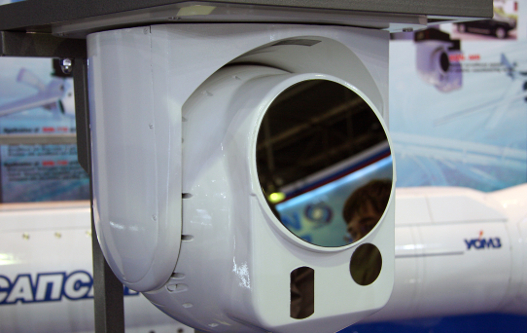
\includegraphics[width=0.7\linewidth]{p1} 
 \caption{Оптико-электронная система СОН-730}
 \label{fig:soep}
\end{figure}

Радикальным преимуществом \hyperref[acroEOS]{ОЭС} по сравнению с радиолокационными является также и гораздо более высокая скрытность их работы, что существенно повышает выживаемость  \hyperref[acroLA]{ЛА} в ходе проведения ими боевых действий. 

Однако у этих систем есть большой недостаток по сравнению с радиолокационными существенная зависимость их рабочих характеристик от метеоусловий и невозможность работы через облачность. 

По реализуемым ТТХ многие отечественные авиационные  \hyperref[acroEOS]{ОЭС}, к сожалению, отстают от современного мирового уровня. Это обусловлено, главным образом, более низким качеством отечественной оптико-электронной элементной базы для них и технологического производственного оборудования. Важным фактором достижения успешного конкурентоспособного результата является следование строгой методике разработки и исследования динамики вновь разрабатываемых систем управления бортовыми оптико-электронными приборами, использование информационных технологий для ускорения разработки изделий и уменьшения количества ошибок. Отсутствие процесса моделирования системы управления во время разработки прибора может снижать общую надежность изделия.

Крайне важно видеть наиболее перспективные направления совершенствования отечественной оптико-электронной техники выбирая наиболее перспективные направления как по степени их приоритетности, так и по минимуму технических рисков. 

В этой связи для разработчиков и потребителей отечественных  \hyperref[acroLA]{ЛА} значительный интерес представляют данные по серийным авиационным оптико-электронным системам, используемым в настоящее время в зарубежной авиационной практике. Одновременно для них представляют интерес и тенденции совершенствования этих систем для понимания в каких направлениях целесообразно продвигаться дальше. 

Целью данного обзора является представление информации по этим вопросам, а также сравнительный анализ представленных систем по критерию выполняемой боевой задачи. 

\section{Обзорно-поисковые, прицельные и пилотажные оптико-электронные системы} \label{sec:ch1/sec1-}

Для создания  \hyperref[acroEOS]{ОЭС} смотрящего типа базирующейся на  \hyperref[acroLA]{ЛА} рассмотрим некоторые аналогичные приборы зарубежного и Российского производства. Таблица \ref{tab:EOS} демонстрирует зарубежные и российские авиационные обзорно-поисковые, прицельных и пилотажных оптико-электронных систем ( \hyperref[acroEOS]{ОЭС}), произведенные за последние 10 лет. 

\begin{landscape}

\begin{longtable}{| p{6cm} | p{18cm} |}
	\caption{Поисково-следящие системы авиационного базирования}%
	\label{tab:EOS}% label всегда желательно идти после caption
	\\ \hline
		Название комплекса, 
		
		Страна производитель, 
		
		Год начала производства, 
		
		Масса 
		& 
		Описание 
	\\ \hline
		OSF (Optronique Secteur Frontal). Thales Optronics, SAGEM, \cite[]{OSF}
		
		Франция, 
		
		2010 г., 
		
		95 кг. 
	& 
		ДТВ, 3-5 + 8-12 мкм-IRST, ЛД-1,54. Установлена в верхней носовой части самолета перед кабиной фюзеляжа выведены 2 раздельные IRST- и ДТВ + ЛД-головки. Последняя является ОМБ ОП-подсистемы "CIU" (Combat Identification Unit), предназначенной как для наведения на воздушные цели УР "воздух-воздух", так и для решения прицельных задач по земле, воде. 
		IRST-подсистема обеспечивает круглосуточное обнаружение и распознавание воздушных целей, имеет ТпВ-режим. Фотоматериал и топология используемых в ней фоточувствительных элементов не сообщаются (по косвенным данным, в обоих диапазонах используются сканирующие 4х288 эл.-субматрицы). 
		
		
		Днем для более точного распознавания и идентификации этих целей используется узкопольный ДТВ из состава ОП-подсистемы "CIU". Со временем планируется заменить его на круглосуточную ТВ-камеру. По имеющимся данным, дальность обнаружения воздушных целей IRST-подсистемой составляет Rо 80...100 км, ДТВ 30...50 км, типовых наземных целей соответственно 40 (в ТпВ-режиме) и 35 км. 
		
		Основную же нагрузку при решении ударных задач по земле, воде несет уже приводившаяся ранее, также предназначенная для использования на самолете Rafale контейнерная ОПС "DAMOCLES".
	\\ \hline
		IR OTIS. Saab Bofors Dynamics \cite[]{doi:10.1117/12.450557},
		
		Швеция	
		
		2010 г,	
		
		30-10 кг
		 
	& 
		Встроенная 8-12 мкм-IRST + ОП-система для шведского самолета Jas 39 Gripen. 
		Данная система предназначена для работы по воздуху и земле. В ней используется сканирующий фотоприемник с числом элементов nэл 1200, фоточувствительный материал и топология расположения элементов не сообщаются (по косвенным данным, это 4х288 эл-КРТ-субматрица). Она может работать как с широкими полями зрения для быстрого обзора, так и с узкими для обнаружения целей на больших дальностях. Опять же по косвенным данным, эти поля равны 12х12 / 5,5х5,5 / 2х2о. 
		Сектора обзора могут выставляться оператором в заданных направлениях в пределах передней полусферы самолета. Система может работать в IPST-режиме сразу по многим целям "на проходе" и в ТпВ-режиме осуществлять точное АС выбранной цели. 
		ОМБ установлен на верхней носовой части фюзеляжа самолета, перед кабиной, несколько левее строительной оси самолета для обеспечения ограниченного обзора земной поверхности. 
		 
	\\ \hline
		Strix / Nightowl. SAGEM	
		
		Франция	
		
		2000 г. 	
		
		105 кг 
	& 
		Для французского эскортного вертолета Tigre HAP. Надкабинное размещение, также может наводить на цели ПТУР "HOT" и "Hellfire". 
		Оптический визир (ОВ), 3х-польные ДТВ, 8-12 мкм-ТпВ-II, ЛД-1,54, ИК-пеленгатор ПТУР "HOT", 
		может быть ЛДЦ-1,06 / 1,54, ПЛП. Может наводиться на цели от НСЦИ пилота. В ТпВ используется сканирующая 4х288 эл.-КРТ-субматрица, мини ЭЛТ вводит ДТВ- и ТпВ-изображения в окуляр ОВ (возможна модификация и без ОВ). 
		При изготовлении корпуса ОМБ этой ОПС используются облегченные композитные материалы, что 
		крайне важно для надкабинного конструктивного исполнения.
		 
	\\ \hline
		M-TADS / PNVS. Lockheed Martin, DRS Technologies
		\cite[]{lockheedmartin}
		
		США	
		
		2005 г. 
		 
	& 
		ОП + пилотажная  \hyperref[acroEOS]{ОЭС} американского армейского вертолета AH-64D Apache Longbow. Носовое размещение. 
		В состав ОП-подсистемы "M-TADS" входят ч/б ДТВ, 3-5 мкм-ТпВ-III, 8-12 мкм-ТпВ-II, ЛДЦ-1,06 / 1,54, ПЛП, ИНС / GPS, в состав пилотажной подсистемы "M-PNVS" широкопольные НУТВ и 8-12 мкм-ТпВ-II. 
		В 8-12 мкм-ТпВ-II-каналах обеих подсистем используются сканирующие 4х480 эл.-КРТ-субматрицы, 
		в 3-5 мкм-ТпВ-III-канале ОП-подсистемы смотрящая 320х256 эл.-InSb-матрица + микроскан (nэл
		экв= 640х512). Последний размещен в одном отсеке с ДТВ, при этом отсек имеет прозрачное для обоих этих каналов сапфировое входное окно. 
		В обеих подсистемах предусмотрены интегрирование ТВ- и ТпВ-изображений, выдача их на НСЦИ 
		пилотов и, в оцифрованном виде, на землю и на другие  \hyperref[acroLA]{ЛА}.
		 
	\\ \hline
		CоMPASS.		
		
		2001 г. 	
		
		38 - 35 кг 
& 
Панкратический ч/б или цветной ДТВ, 3х-польный 3-5 мкм-ТпВ-III, ЛД-1,54 или ЛЦУ-1,06, ПЛП, 0,8 
мкм-лазерный маркер. Может быть 8-12 мкм-ТпВ-II. В 3-5 мкм-ТпВ используется 320х256 эл.-InSb-матрица + микроскан (nэлэкв = 640х512), он может быть 
панкратическим. В 8-12 мкм-ТпВ используются сканирующая 4х288 эл.-КРТ-субматрица и дискретные 
поля зрения. ЛД-1,54 на Er-стекле, в ЛЦУ-1,06 используется ППЛ-накачка. Его энергия в импульсе Еи 80 мДж, частота повторения Fи 20 Гц. Мощность излучения маркера Ризл 50 мВт. 
 
\\ \hline
		D-CоMPASS.
				
		2005 г. 
			
		32 - 41 кг 
& 
Могут быть ч/б или цветной ДТВ, 3-5 мкм-ТпВ-III, 8-12 мкм-ТпВ-II, ЛД-1,54, ЛДЦ-1,06 / 1,54 с ППЛ- 
накачкой его лазерного излучателя, ПЛП, 0,8 мкм-лазерный маркер, ИНС / GPS-блок. 
Варианты ДТВ: 
панкратические ч/б или цветной, панкратический цветной, на более крупноформатной (1,3 мп) матрице, широкопольный с полем зрения по горизонтали г = 24о. 
Варианты ТпВ: 
3-5 мкм-ТпВ-III на 640х512 эл.-InSb-матрице, с фиксированными полями зрения ( у = 0,67х 0,5о), то же самое, но с панкратическим изменением промежуточных i , 3-5 мкм-ТпВ-III на 320х256 эл.-InSb-матрице, с более широкими i , 8-12 мкм-ТпВ-II на сканирующей 4х288 эл.-КРТ-субматрице, с более широкими i . 
ИНС / GPS-блок обеспечивает высокоточную навигацию  \hyperref[acroLA]{ЛА}, задаваемые режимы обзора пространства, выработку абсолютных координат (геолокацию) целей, многоканальное их АС 
. Видеоизображения и символика могут выдаваться на ИЛС или на НСЦИ пилота. 
 
\\ \hline
	SEOS. Saab Bofors Dynamics \cite[]{doi:10.1117/12.450557}
	
	Швеция	
	
	2005 г. 	
	
	70 кг	 
& 
ДТВ, 8-12 мкм-ТпВ-II, ЛД-1,54. Могут быть НУТВ, 3-5 мкм-ТпВ-III, ИК-пеленгатор ПТУР, ЛЦУ-
1,06, лазерно-лучевой канал управления (ЛЛКУ) ПТУР.
Есть улучшение качества и интегрирование между собой ДТВ- и ТпВ-изображений.
 
\\ \hline
		OLOSP. SAGEM
		\cite[]{sagem-olosp}
		
		Франция		25 кг
		 
		40 кг. 
		 
& 
Могут быть панкратический цветной ДТВ, высокоразрешающий ч/б ДТВ, 3-5 мкм-ТпВ-III, 8-12 мкм-ТпВ-II, ЛД-1,54, радиолиния передачи информации на землю. 
ДТВ построен по 3х-матричной схеме формирования цветности, 3-5 мкм-ТпВ на 640х512 эл.-КРТ-матрице, 8-12 мкм-ТпВ на сканирующей 4х288 эл.-КРТ-субматрице. 
 
\\ \hline
		EUROFLIR 410. SAGEM
		\cite[]{EUROFLIR}
		Франция, Technobit, Испания	2008 г	45 кг
		 
& 
Модульная система. Могут быть различные варианты с панкратическими мегапиксельным цветным 
ДТВ, ч/б НУТВ, 3-5 мкм-ТпВ-III или 8-12 мкм-ТпВ-II, 0,15о
-спотоскопом, ЛД-1,54, ЛЦУ-1,06, 0,8 мкм-лазерным маркером. 3-5 мкм-ТпВ на 640х512 эл.-КРТ-матрице, 8-12 мкм-ТпВ на сканирующей 4х288 эл.-КРТ-субматрице.
 
\\ \hline
		FIN 1010 AN / AAR-51. Selex Galileo	
		
		Англия		 
& 
Для самолетов английских ВВС и американского Корпуса морской пехоты (КМП). Может использоваться также и на военно-транспортных и гражданских самолетах. Может быть в контейнерном и во встроенном конструктивных исполнениях. 
В ТпВ используется 8 эл.-КРТ SPRITE, = 25х16о, ТпВ-изображение выводится на кабинный ИЛС. 
 
\\ \hline
		Pathfinder. Lockheed Martin	
		
		США		
		
		90 кг. 
& 
Создан на базе навигационного контейнера "AN / AAQ-13" довольно популярной в прошлом самолет-
ной ОП + пилотажной  \hyperref[acroEOS]{ОЭС} "LANTIRN" с исключением из него 3 см-навигационой РЛС. 
Так же, как и раньше, в ТпВ используется сканирующая однорядная 180 эл.-КРТ-линейка, в отличие 
от ТпВ упомянутого контейнера теперь используется не одно, а 2 поля зрения ш / у = 28х21 / 9х7о
, уз-
кое поле предназначено для обнаружения наземных целей. 
\\ \hline
		Sure Sight EVS. CMC Electronics Inc.	
		
		США	2001 г	
		
		8,2-1,8 кг
		 
& 
Enhanced Vision System предназначена для использования на борту военно-транспортных и гражданских бизнес-самолетов с целью обеспечения круглосуточного "видения" их пилотами обстановки в аэропорту при взлете-посадке, маневрировании на земле в условиях ухудшенной видимости (ночью, в осадках, тумане и т.п.). 
Сначала в этой системе использовался только ТпВ-канал, потом, в качестве опции, был добавлен мм-рл-канал. ТпВ размещен в обтекателе метеоРЛС, "смотрит" вперед через ИК-прозрачное окно. Может быть размещен и под или над обтекателем мм-рл-канала. ТпВ- и рл-изображения в проинтегрированном (синтезированном) виде выводятся на самолетный ИЛС. Есть 2 варианта построения ТпВ-канала: - 8-12 мкм-ТпВ-II на криогенно охлаждаемой сканирующей 4х288 эл-КРТ-субматрице, имеет высокую чувствительность, дает качественное изображение, масса m = 8,2 кг, 
-более дешевый 8-14 мкм-ТпВ-III на неохлаждаемой 320х240 эл.-матрице, m = 1,8 кг, может размещаться в носу  \hyperref[acroLA]{ЛА} или быть встроен его хвостовое оперение.
 
\\ \hline
		PACIS. Selex Galileo
		
		Англия		
		
		33 кг 
& 
Помимо пилотажных задач может решать и прицельные. Используется 8 эл.-КРТ-SPRITE, поля зрения ш / у = 40х30 / 10х6,6о, кадровая частота Fк = 25 Гц/ 
\\ \hline
	AN / AAQ-18. Raytheоn	
	
	США		 
& 
Используется сканирующая 120 эл.-КРТ-линейка, ш / у = 18х14 / 4х3о 
\\ \hline
	Pathfinder. Lockheed Martin	
	
	США	
	
	2009 г.	
	
	50 кг 
& 
Для транспортных вертолетов общего назначения CH-47 Chinook и UH-60 Black Hawk. Устанавливается в носу вертолета.
Данная  \hyperref[acroEOS]{ОЭС} была создана на базе пилотажной подсистемы "M-PNVS" американского боевого вертолета AH-64D Apache Longbow по разд.2. В ТпВ-канале используется сканирующая 4х480 эл.-КРТ-субматрица, разворачиваемая в две горизонтальные полосы с формированием в кадре N = 1728х960 элементов разложения (пикселей). Поле зрения равно = 52х30о. НУТВ- и ТпВ-изображения интегрируются между собой и выдаются на НСЦИ пилота. НУТВ может "видеть" искусственные световые источники, что облегчает пилотаж, а также подсвет от сухопутных лазерных маркеров, что улучшает взаимодействие с СВ. 
 
\\ \hline
	NOCTUA. Thales Optronics	
	
	Англия, Cumulus, ЮАР		
	
	24,5 кг 
& 
Для южноафриканского боевого вертолета Rooivalk. Используется сканирующая 4х288 эл-КРТ-субматрица, = 40х30о, ТпВ-изображение выдается на НСЦИ пилота, управляющую визирной осью ТпВ со ср. кв. ошибкой 18'. 
\\ \hline
	FLIR III. AIM	
	
	Германия		
	
	20 кг. 
& 
Для немецких вертолетов Tiger, NH 90 TTH. Используется сканирующая 4х288 эл-КРТ-субматрица, = 40х30о, ТпВ-изображение выдается на НСЦИ пилота. 
\\ \hline

\end{longtable}

\end{landscape}

По приведенным в таблице данным можно сделать некоторые выводы: 

\begin{enumerate}
	\item Опыт проведения странами НАТО боевых действий в ряде военных кампаний последних лет показал целесообразность возложения на обзорно-поисковые и прицельные  \hyperref[acroEOS]{ОЭС}- самолетов, вертолетов и  \hyperref[acroUAV]{БЛА} не только собственно разведывательно-прицельных задач, но и информационной поддержки своих наземных подразделений СВ и ВМС в части обеспечения их большей осведомленности относительно поведения противника в зоне проводимых ими боевых действий.
	\item С этой целью в состав оборудования  \hyperref[acroEOS]{ОЭС} в последние годы стали включать лазерные маркеры для выдачи ЦУ наземным пользователям при ведении боевых действий в темное время суток. Сами же  \hyperref[acroLA]{ЛА} стали оснащаться линиями передачи изображений высокой четкости, на другие  \hyperref[acroLA]{ЛА}, участвующие вместе с ними в совместных боевых операциях, и т.п.
	\item В настоящее время наметилась устойчивая тенденция оснащения авиационных  \hyperref[acroEOS]{ОЭС} датчиками высокого разрешения, имеющими ряд существенных технических и тактических достоинств. Так, они позволяют: использовать в этих датчиках менее габаритную (более короткофокусную) оптику; обеспечивать более высокие вероятностные характеристики обнаружения объектов; сократить временные затраты на распознавание последних. 
	\item Наиболее популярными в авиационных  \hyperref[acroEOS]{ОЭС} ТпВ-датчиками являются:
	\begin{enumerate}
		\item 3...5-мкм ТпВ 3-го поколения (ТпВ-III) на не сканирующих ("смотрящих") матрицах на криогенно охлаждаемых антимониде индия (InSb) и кадмии-ртуть-теллуре (КРТ); 
		\item 8...12 мкм ТпВ 2-го поколения (ТпВ-II) на сканирующих КРТ-субматрицах, реже 8...12-мкм ТпВ-III на смотрящих КРТ-матрицах и еще реже 8...9-мкм ТпВ-III на смотрящих матрицах на арсениде галлия (GaAs); 
		 
		
		\item 8...12-мкм ТпВ-III на неохлаждаемых матрицах (чаще всего используются при решении наблюдательных задач).
	\end{enumerate}
	\item На боевых вертолетах сухопутной поддержки, зачастую работающих в условиях помех и разрывов боеприпасов на поле боя, преобладающими являются 8...12-мкм ТпВ-датчики, особенно если вертолеты предназначены для эксплуатации как в теплых, так и в холодных климатических зонах. В наиболее совершенных  \hyperref[acroEOS]{ОЭС} используются оба спектральных диапазона. 
	\item На всех типах  \hyperref[acroLA]{ЛА} все большую популярность в последние годы приобретают панкратические цветные ДТВ, такие же ТпВ, сверхузкопольные ДТВ (спотоскопы), а лазерные маркеры. 
	\item Использование спотоскопов и маркеров стало возможным благодаря реализации в уникальных точностей стабилизации линий визирования входящих в их состав прицельных каналов (стаб 1...20") .
	\item В плане проведения модернизаций авиационных  \hyperref[acroEOS]{ОЭС} следует предусматривать осуществление следующих технических мероприятий: 
	\begin{enumerate}
		\item переход в самолетных интегрированных  \hyperref[acroEOS]{ОЭС} от контейнерного на встроенное конструктивное исполнение; 
		\item перевод лазерных излучателей ЛД, ЛЦУ с широкополосной ламповой на гораздо более эффективную по промышленному кпд узкополосную полупроводниковую накачку; 
		\item интегрирование между собой ДТВ-, НУТВ- и ТпВ-изображений; 
		\item применение вторичной цифровой обработки выходных видеосигналов этих датчиков с целью улучшения качества выдаваемых ими изображений перед предъявлением их летчикам, а также формирование по ним некоторого нового изображения с использованием преимуществ каждого из датчиков в той или иной обстановке; 
		\item введение в состав  \hyperref[acroEOS]{ОЭС} собственных, инерциально-навигационных системных блоков для повышения точностей углового автосопровождения целей
		\item при использовании информации от бортовых GPS-приемников и ЛД, выдачи высокоточных координат этих целей в систему управления оружием "дальней руки", другим внешним по отношению к  \hyperref[acroLA]{ЛА} потребителям. 
	\end{enumerate}
\end{enumerate}

\section{Авиационные оптико-электронные системы инфракрасного противодействия ракетной атаке} \label{sec:ch1/sec2-}

Для излучающей  \hyperref[acroEOS]{ОЭС} базирующейся на  \hyperref[acroLA]{ЛА} также рассмотрим некоторые аналогичные приборы зарубежного и Российского производства. Далее приведены зарубежные и российские авиационные оптико-электронные системы инфракрасного противодействия ракетной атаке. Можно выделить 3 поколения систем оптико-электронного подавления ( \hyperref[acroSOEP]{СОЭП}):

\begin{enumerate}
	\item Системы всенаправленной постановки помех
	\item Системы с узконаправленным пучком постановки помех
	\item Лазерные системы противодействия 	
\end{enumerate}

В состав системы противодействия ракетной атаке входят несколько подсистем. Состав расписан на рисунке \ref{fig:classification}.

\begin{figure}[ht]
	\centering
	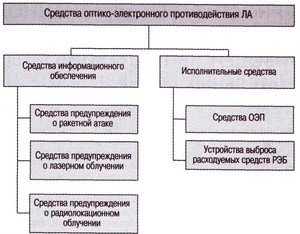
\includegraphics[width=0.6\linewidth]{p2} 
	\caption{Классификация средств  \hyperref[acroSOEP]{СОЭП}  \hyperref[acroLA]{ЛА} \cite[]{ForeignMilitary}}
	\label{fig:classification}
\end{figure}

В составе исполнительных средств указаны “средства ОЭП”, система управления для этой подсистемы комплекса рассматривается в настоящей работе. Генератор пульсирующих инфракрасных помех представляет собой мощную инфракрасную лампу с вращающимся отражателем или способную изменять свою яркость с заданной частотой, в кожухе из прозрачного для инфракрасного излучения материала.

Ракеты с инфракрасной головкой самонаведения (\hyperref[acroGSN]{ГСН}) относятся к самым простым управляемым средствам поражения воздушных целей. Принцип сканирования поля зрения \hyperref[acroGSN]{ГСН} показан на рисунке \ref{fig:rocketScanning}. 

\begin{figure}[ht]
	\centering
	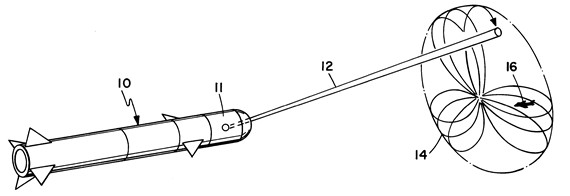
\includegraphics[width=0.7\linewidth]{p3} 
	\caption{Принцип сканирования головкой самонаведения ракеты}
	\label{fig:rocketScanning}
\end{figure}

\begin{itemize}
	\item 10 – ракета с \hyperref[acroGSN]{ГСН}
	\item 11 – сканирующая система в составе \hyperref[acroGSN]{ГСН}
	\item 12 – сектор моментального поля зрения
	\item 14 – полное поле зрения \hyperref[acroGSN]{ГСН}
	\item 16 – цель (летательный аппарат)	
\end{itemize}
	
При генерировании пульсирующих инфракрасных помех с частотой, равной рабочей частоте внутренних элементов наведения, и мощностью, сопоставимой с естественным тепловым излучением защищаемой цели, в систему наведения ракеты вносится помеха, приводящая к отклонению ракеты от защищаемой цели. Вероятность срыва атаки ракеты ПЗРК при использовании генераторов пульсирующих инфракрасных помех составляет от 0,5 до 0,7-0,8.

\subsection{ \hyperref[acroSOEP]{СОЭП} первого поколения}	

К  \hyperref[acroSOEP]{СОЭП} первого поколения относятся системы ненаправленной постановки помех. Такие системы не представляют интереса для проводимой работы так как не имеют системы наведения. Принцип действия станции основан на генерации всенаправленного модулированного помехового ИК-излучения со специальной структурой сигнала. К таким системам относятся \cite[]{SOEP_LIPA}:

\begin{itemize}
	\item «Липа» (РФ)	
	\item AN/ALQ-144 (США, смотри рисунок \ref{fig:alq})	
	\item AN/ALQ-157 by BAE Systems, used for larger helicopters and aircraft.
	\item AN/ALQ-212 by BAE Systems, currently fielded on U.S. Army CH-47 Chinook helicopters.
	\item “Адрос КТ-01 АВ” (Украина)
	\item “Квадрос-КМ-01 В” (Украина) 		
\end{itemize}

\begin{figure}[ht]
	\centering
	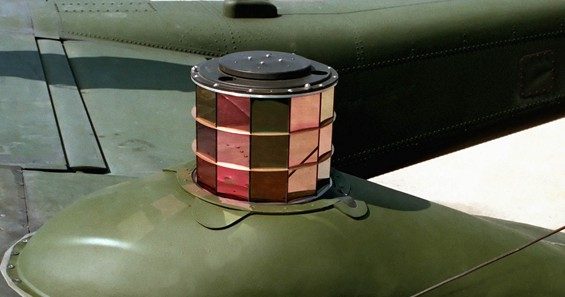
\includegraphics[width=0.7\linewidth]{p4} 
	\caption{ \hyperref[acroSOEP]{СОЭП} первого поколения}
	\label{fig:alq}
\end{figure}
На рисунке \ref{fig:alq} показана система постановки всенаправленных помех AN/ALQ-144 установленная на борту летательного аппарата. Устройство не имеет подвижных частей, ИК излучение от источника проходит через фильтр и распространяется в верхней полусфере.

 \hyperref[acroSOEP]{СОЭП} первого поколения обеспечивают защиту военной авиационной техники от ракетных комплексов с инфракрасными головками самонаведения (ИК \hyperref[acroGSN]{ГСН}) типа «Сайдуиндер», «Ред Ай», «Чапарэл», «Питон», «Стрела-2М», «Хунинь-5» и им подобных. 

\subsection{ \hyperref[acroSOEP]{СОЭП} второго поколения}	

К  \hyperref[acroSOEP]{СОЭП} второго поколения относятся системы с узконаправленным ОЭП (DIRCM) модулированным пучком помехового излучения. Примеры приведены на рисунках ниже (рисунок \ref{fig:p6}, рисунок \ref{fig:p7}).

В состав комплекса входит станции предупреждения о ракетной атаке, имеющие ряд общих особенностей:
\begin{itemize}
	\item модульность конструкции, сравнительно малая масса (7-17 кг) и размеры;
	\item потребляемая мощность порядка 70-100 Вт;
	\item обнаружение атакующих ракет в секторах до 360° в азимутальной и до 180° в угломестной плоскости на дальности 3-10 км с угловым разрешением порядка 1° или меньше;
	\item в большинстве станций используются датчики, функционирующие в УФ-диапазоне ЭМВ.
\end{itemize}

Принцип работы  \hyperref[acroSOEP]{СОЭП} узконаправленным пучком основан на раннем обнаружении пуска ракеты, ее сопровождении и подавлении канала наведения с использованием узконаправленного потока модулированного ИК излучения. Работа средств направленного оптико-электронного противодействия ракетной атаке осуществляется в следующей последовательности (смотри рисунок \ref{fig:p5}) \cite[]{ForeignMilitary}:

\begin{enumerate}
	\item Обнаружение атакующей УР средствами информационного обеспечения в диапазонах 0,01-0,4 мкм (УФ) и 4-14 мкм (ИК).
	\item ОЭП ИК \hyperref[acroGSN]{ГСН}, формирование ложного сигнала от цели. 
	\item Срыв наведения на цель. 
	\item Цель вне поля зрения \hyperref[acroGSN]{ГСН} УР. 
	\item УР не представляет угрозы для вертолета.	
\end{enumerate}

\begin{figure}[ht]
	\centering
	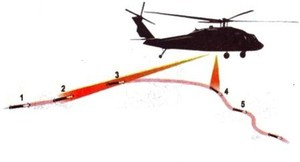
\includegraphics[width=0.6\linewidth]{p5} 
	\caption{Схема работы  \hyperref[acroSOEP]{СОЭП} при атаке ракетой с головкой самонаведения}
	\label{fig:p5}
\end{figure}

Использование нескольких излучателей, размещенных на  \hyperref[acroLA]{ЛА}, ЦСУ и оперативного перепрограммирования режимов работы значительно увеличивает вероятность противодействия угрозе ракетной атаки.

\begin{figure}[ht]
	\centering
	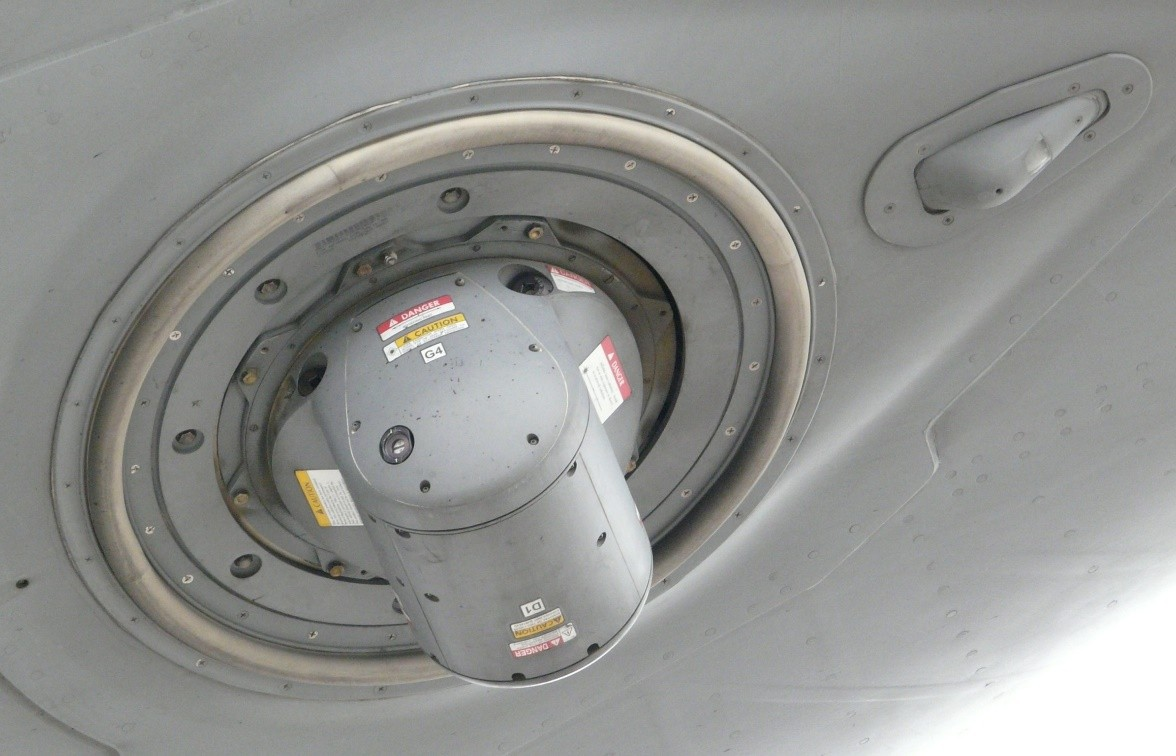
\includegraphics[width=0.6\linewidth]{p6} 
	\caption{ \hyperref[acroSOEP]{СОЭП} пульсирующих инфракрасных помех}
	\label{fig:p6}
\end{figure}


К  \hyperref[acroSOEP]{СОЭП} такого типа относятся \cite[]{Infrared_countermeasure}:
\begin{itemize}
	\item Президент-С;
	\item Leonardo’s Miysis DIRCM (directed infrared countermeasure);
	\item AN/AAQ-24 by Northrop Grumman – DIRCM;
	\item AN/ALQ-132 by Sanders/BAE Systems. Used in the 1960s in Vietnam, and was a fuel fired flashlamp system;
	\item CAMPS by Saab Avitronics, used for civilian and VIP aircraft;
	\item CIRCM by Northrop Grumman;
	\item Flight Guard by Israel Aerospace Industries, used in military and civilian aircraft (gain the nickname of "Live Saver" due to history of success in saving air vehicles during battles at several countries), but banned at several European airports. According to defense sources in Israel, the European ban is "odd and based mostly on a misunderstanding;
	\item ITT's CIRCM System;
	\item Selex ES' Miysis System;
	\item "Sukhogruz" - Russian DIRCM (used on Su-25T);
	\item KT-01 AVE and KT-02 ACE by Adron, used for military aircraft.		
\end{itemize}

\begin{figure}[ht]
	\centering
	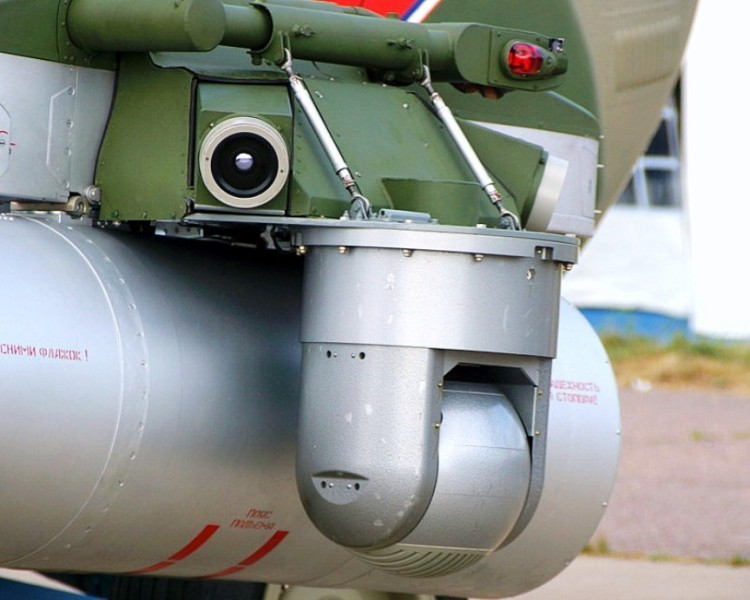
\includegraphics[width=0.5\linewidth]{p7} 
	\caption{Станция Л370-5 и УФ пеленгатор пуска ракет Л370-5-02}
	\label{fig:p7}
\end{figure}

\subsection{ \hyperref[acroSOEP]{СОЭП} третьего поколения}	
К  \hyperref[acroSOEP]{СОЭП} последнего поколения относятся лазерные системы защиты. Основными преимуществами таких систем являются независимость эффективности системы оптико-электронных помех от принципа работы головок наведения у ракет, меньший вес и габариты по сравнению с комплексами второго поколения. Визуальный облик показан на рисунке ниже (рисунок \ref{fig:p8}).

Одним из основных понятий физики взаимодействия лазерного излучения с веществом является порог разрушения. Принято различать два вида порогов разружения – физический и технический. 

Физическим порогом разрушения материала называют такую плотность энергии или мощности (интенсивность) излучения, при которой происходят необратимые изменения оптических характеристик образца (пропускания, рассеяния, отражения) исследуемого материала. Изменение указанных характеристик является следствием образования разрушения, формирование которого сопровождается яркой вспышкой оптического излучения. 

\begin{figure}[ht]
	\centering
	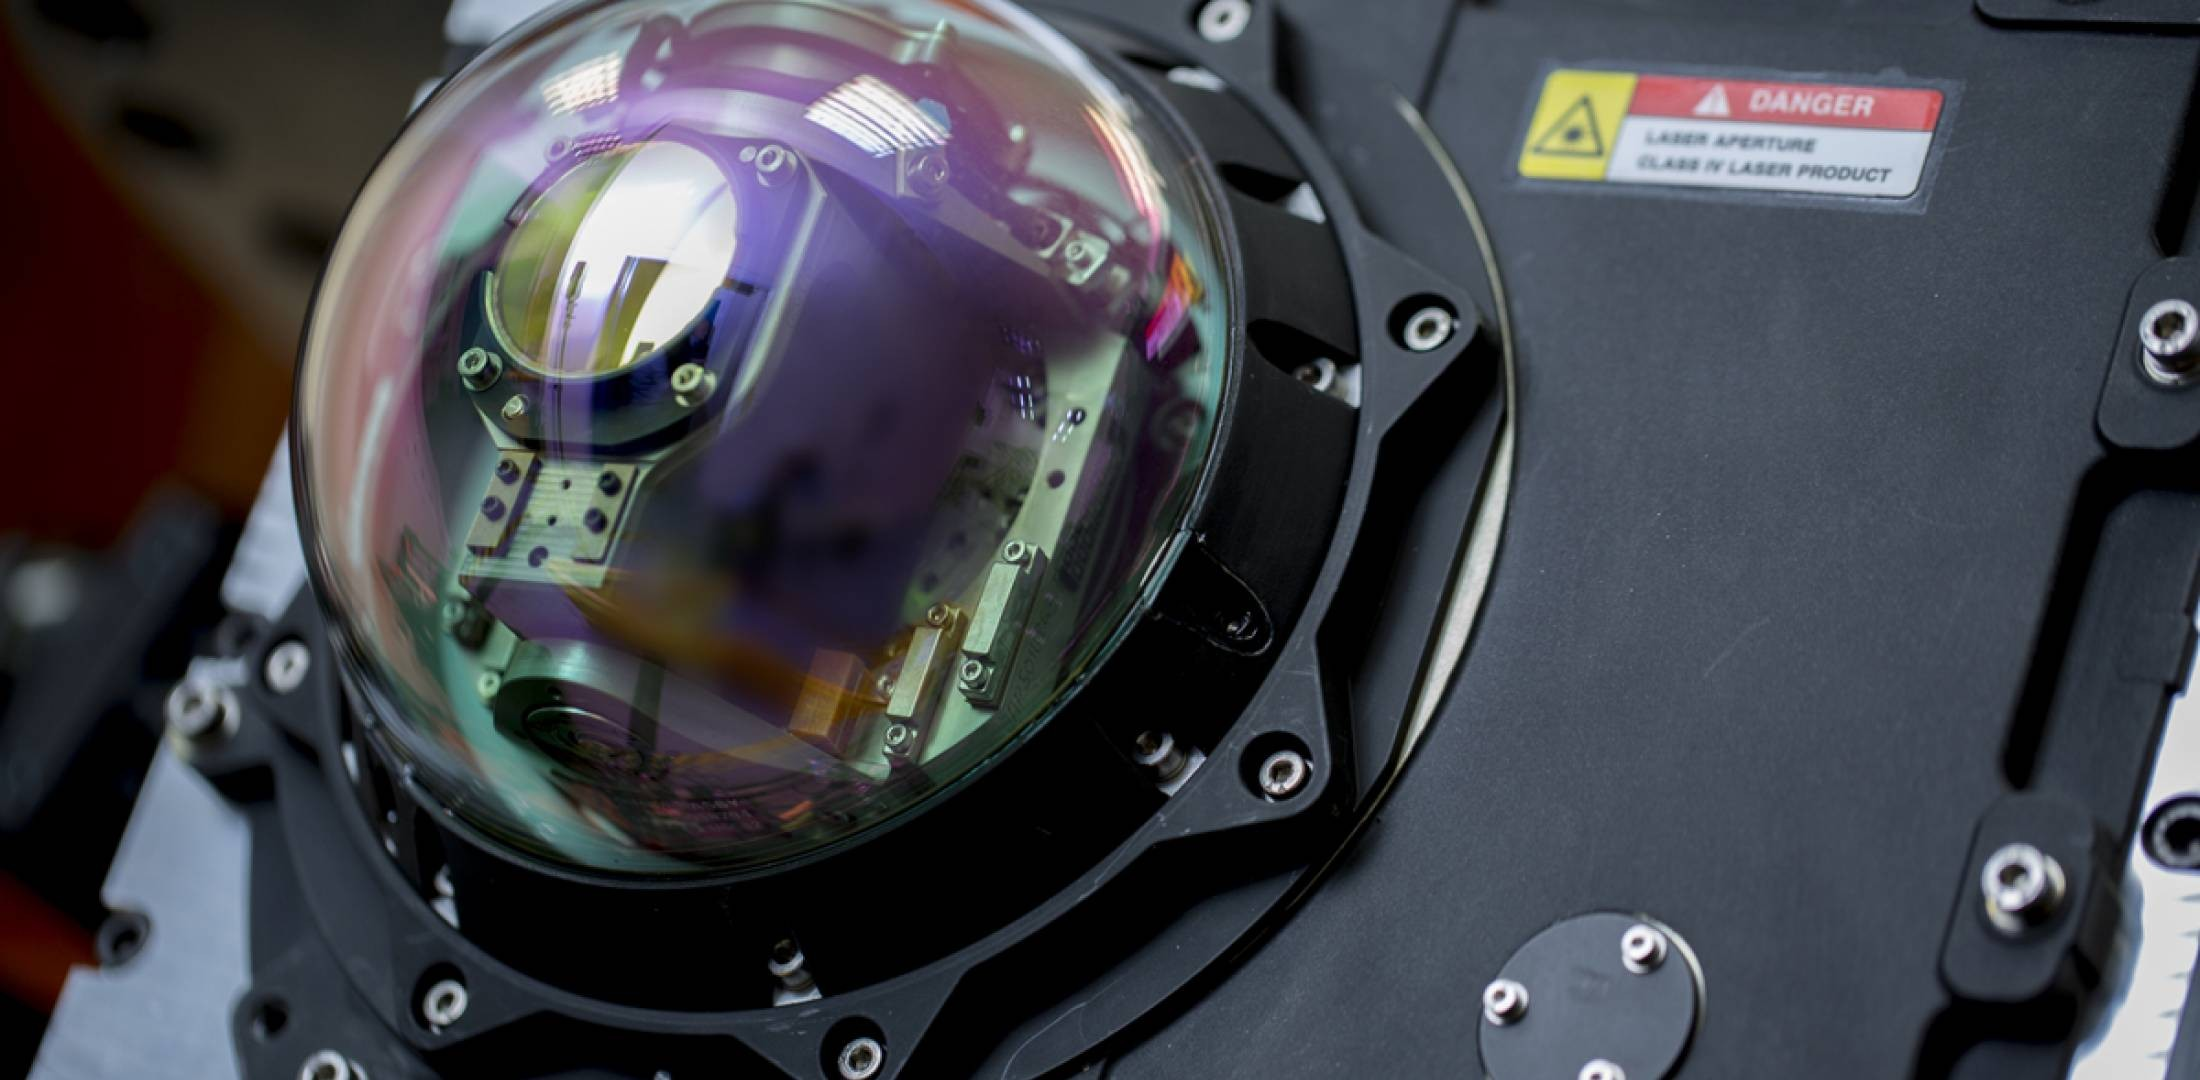
\includegraphics[width=0.8\linewidth]{p8} 
	\caption{Автоматическая бортовая лазерная станция постановки помех ALJS}
	\label{fig:p8}
\end{figure}

Техническим порогом разрушения называют такую плотность энергии или мощности излучения, при которой нарушается работоспособность изделия, изготовленного из исследуемого материала, вследствие изменений его оптических характеристик, превышающих допустимые.

Одним из немногих примеров комплексов третьего поколения является система MANTA (Испания). Это автоматическая бортовая лазерная станция постановки помех ALJS \cite[]{manta}.

Ее работа основывается на использовании кодированного мультиспектрального излучения импульсно-периодического (HF/DF) лазера для создания помех в широком ИК-диапазоне.
Российский комплекс третьего поколения носит название Л370В28, его внешний вид показан на рисунке ниже (рисунок~\ref{fig:p9}). 

\begin{figure}[ht]
	\centering
	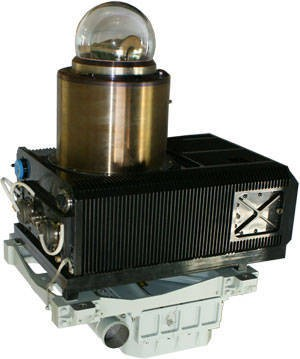
\includegraphics[width=0.4\linewidth]{p9} 
	\caption{Изделие Л370В28 (лазерная станция постановки помех)}
	\label{fig:p9}
\end{figure}

Особенностями средств направленного ОЭП являются \cite[]{ForeignMilitary}:
\begin{itemize}
	\item высокий энергетический потенциал лазерного излучения;
	\item возможность функционального поражения приемных элементов ИК \hyperref[acroGSN]{ГСН}, а также поражения (ослепления) операторов комплексов вооружения и стрелков при наведении лазерного луча на источник угрозы по информации от средств РЭБ ИО;
	\item обеспечение синхронизации со средствами РЭБ ИО для получения информации о направлении на источник угрозы;
	\item необходимость целеуказания на источник угрозы с точностью до нескольких угловых минут;
	\item возможность функционирования в составе систем, включающих несколько станций ОЭП;
	\item возможность совместного функционирования с устройствами выброса расходуемых средств РЭБ.
\end{itemize}



\section{Анализ способов обеспечения обратной связи в современных  \hyperref[acroEOS]{ОЭС}} \label{sec:ch1/sec3-}

Для системы управления наиболее важным элементом является обратная связь. В автоматических оптико-электронных системах рассматриваемых типов управление происходит по углам наведения оптической оси, в качестве датчиков обратной связи углового положения используют следующие типы:
\begin{itemize}
	\item \textbf{СКВТ (Синусно-косинусный вращающийся трансформатор)}
	
	Вращающиеся трансформаторы являются двухобмоточными на статоре (в основном) или многополюсными электрическими машинами. По конструкции аналогичны синхронным электродвигателям с возбуждаемым переменным током ротором. В зависимости от угловой ориентации магнитного поля ротора относительно взаимно перпендикулярным по магнитному потоку обмоток статора в обмотках статора наводится ЭДС, амплитуда и фаза которых зависит от угла поворота ротора относительно статора. Эти электрические сигналы однозначно, в пределах одного оборота ротора, характеризуют угол поворота ротора \cite[]{SKVT}.
	
	\begin{figure}[ht]
		\centering
		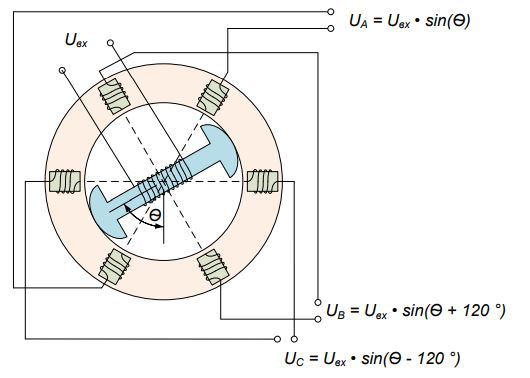
\includegraphics[width=0.5\linewidth]{SKVT} 
		\caption{Принципиальная электромеханическая схема СКВТ \cite[]{1310HM025}}
		\label{fig:SKVT}
	\end{figure}
	
	\item \textbf{Датчик Холла совместно с оптопарой в качестве датчика нуля}

	Магнитный датчик на эффекте Холла регистрируют прохождение магнитных полюсов вращающегося магнитного элемента непосредственно вблизи чувствительного элемента, преобразуя эти данные в соответствующий цифровой код или сигнал \cite[]{Encoder}.
	
	\item \textbf{Энкодер}
	
	Оптические датчики углового положения (\hyperref[acroDUP]{ДУП}) имеют жёстко закреплённый на валу стеклянный диск с оптическим растром. При вращении вала растр перемещается относительно неподвижного растра, при этом модулируется световой поток, принимаемый фотодатчиком. Абсолютные оптические датчики угла — это датчики угла поворота, в которых каждому положению вала соответствует цифровой выходной код, который наряду с числом оборотов является основным рабочим параметром датчика. Абсолютные оптические \hyperref[acroDUP]{ДУПы}, так же как и накапливающие, считывают и фиксируют параметры вращения оптического диска \cite[]{Encoder}.
	
\end{itemize}
С ростом технологичности электронной компонентной базы и появлением возможности обработки изображения в реальном времени для систем смотрящего типа обратную связь можно обеспечить обработкой информации с фотоприемника. Для этого используют:

\begin{itemize}
	\item \textbf{Одноэлементные фотоприемники с применением механических модуляторов}
	
	Для определения координат используется амплитудно-фазовый метод. С помощью анализатора в виде диска с переменной прозрачностью, изменяющейся по закону светового клина. \cite[]{bibook1} Схема работы показана на рисунке~\ref{fig:p10}.
	
	\begin{figure}[ht]
		\centering
		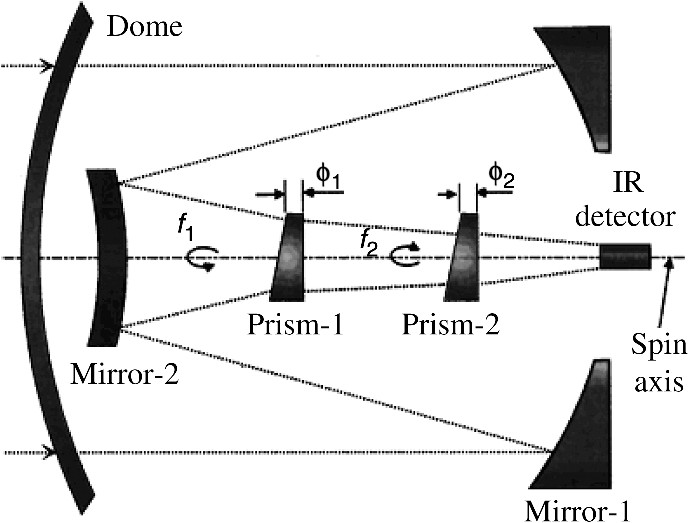
\includegraphics[width=0.6\linewidth]{p10} 
		\caption{Оптическая схема одноэлементной сканирующей \hyperref[acroGSN]{ГСН} }
		\label{fig:p10}
	\end{figure}

	\item \textbf{Позиционно чувстительные фотоприемники}
	
	Приемное устройство представляет собой четырехквадратный фотодиод. Определение отклонения изображения объекта происходит путем вычисления разницы напряжений между элементами. На рисуноке~\ref{fig:4px} показана конструкция фотоприемника.
\newpage	
	\begin{figure}[ht]
		\centering
		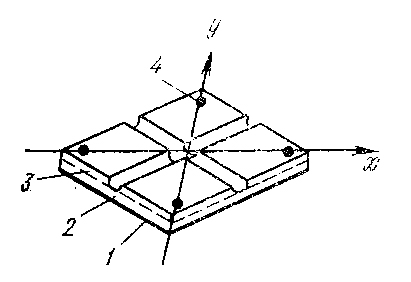
\includegraphics{4px} 
		\caption{Позиционно-чувствительный фотодиод}
		\label{fig:4px}
	\end{figure}
	
	\begin{enumerate}
		\item кристаллодержатель;
		\item \textit{n}-область;
		\item \textit{p}-область;
		\item контакт.
	\end{enumerate}

	\item \textbf{Многоэлементные матричные фотоприемники}
	
	ПЗС-матрица — специализированная аналоговая интегральная микросхема, состоящая из светочувствительных фотодиодов, выполненная на основе кремния, использующая технологию ПЗС — приборов с зарядовой связью. Принципиальная схема показана на рисунке \ref{fig:EMCCD2_color_en}.
	
	ПЗС-матрицы выпускаются и активно используются компаниями Nikon, Canon, Sony, Fujitsu, Kodak, Matsushita, Philips и многими другими. В России ПЗС-матрицы сегодня разрабатывают и выпускают: ОАО «ЦНИИ „Электрон“» (г. Санкт-Петербург) и его дочернее предприятие ЗАО «НПП „Элар“» (г. Санкт-Петербург,) а также ОАО «НПП „Пульсар“» (г. Москва) \cite[]{CCD}.
	
	Наиболее приоритетный тип фотоприёмных устройств на данное время. Повсеместно используется в гражданской продукции, но для данной работы интересны ПЗС матрицы ИК спектра. Далее приведена сравнительная таблица с неохлаждаемыми доступными ПЗС матрицами ИК спектра на рынке.
	
	\begin{figure}[ht]
		\centering
		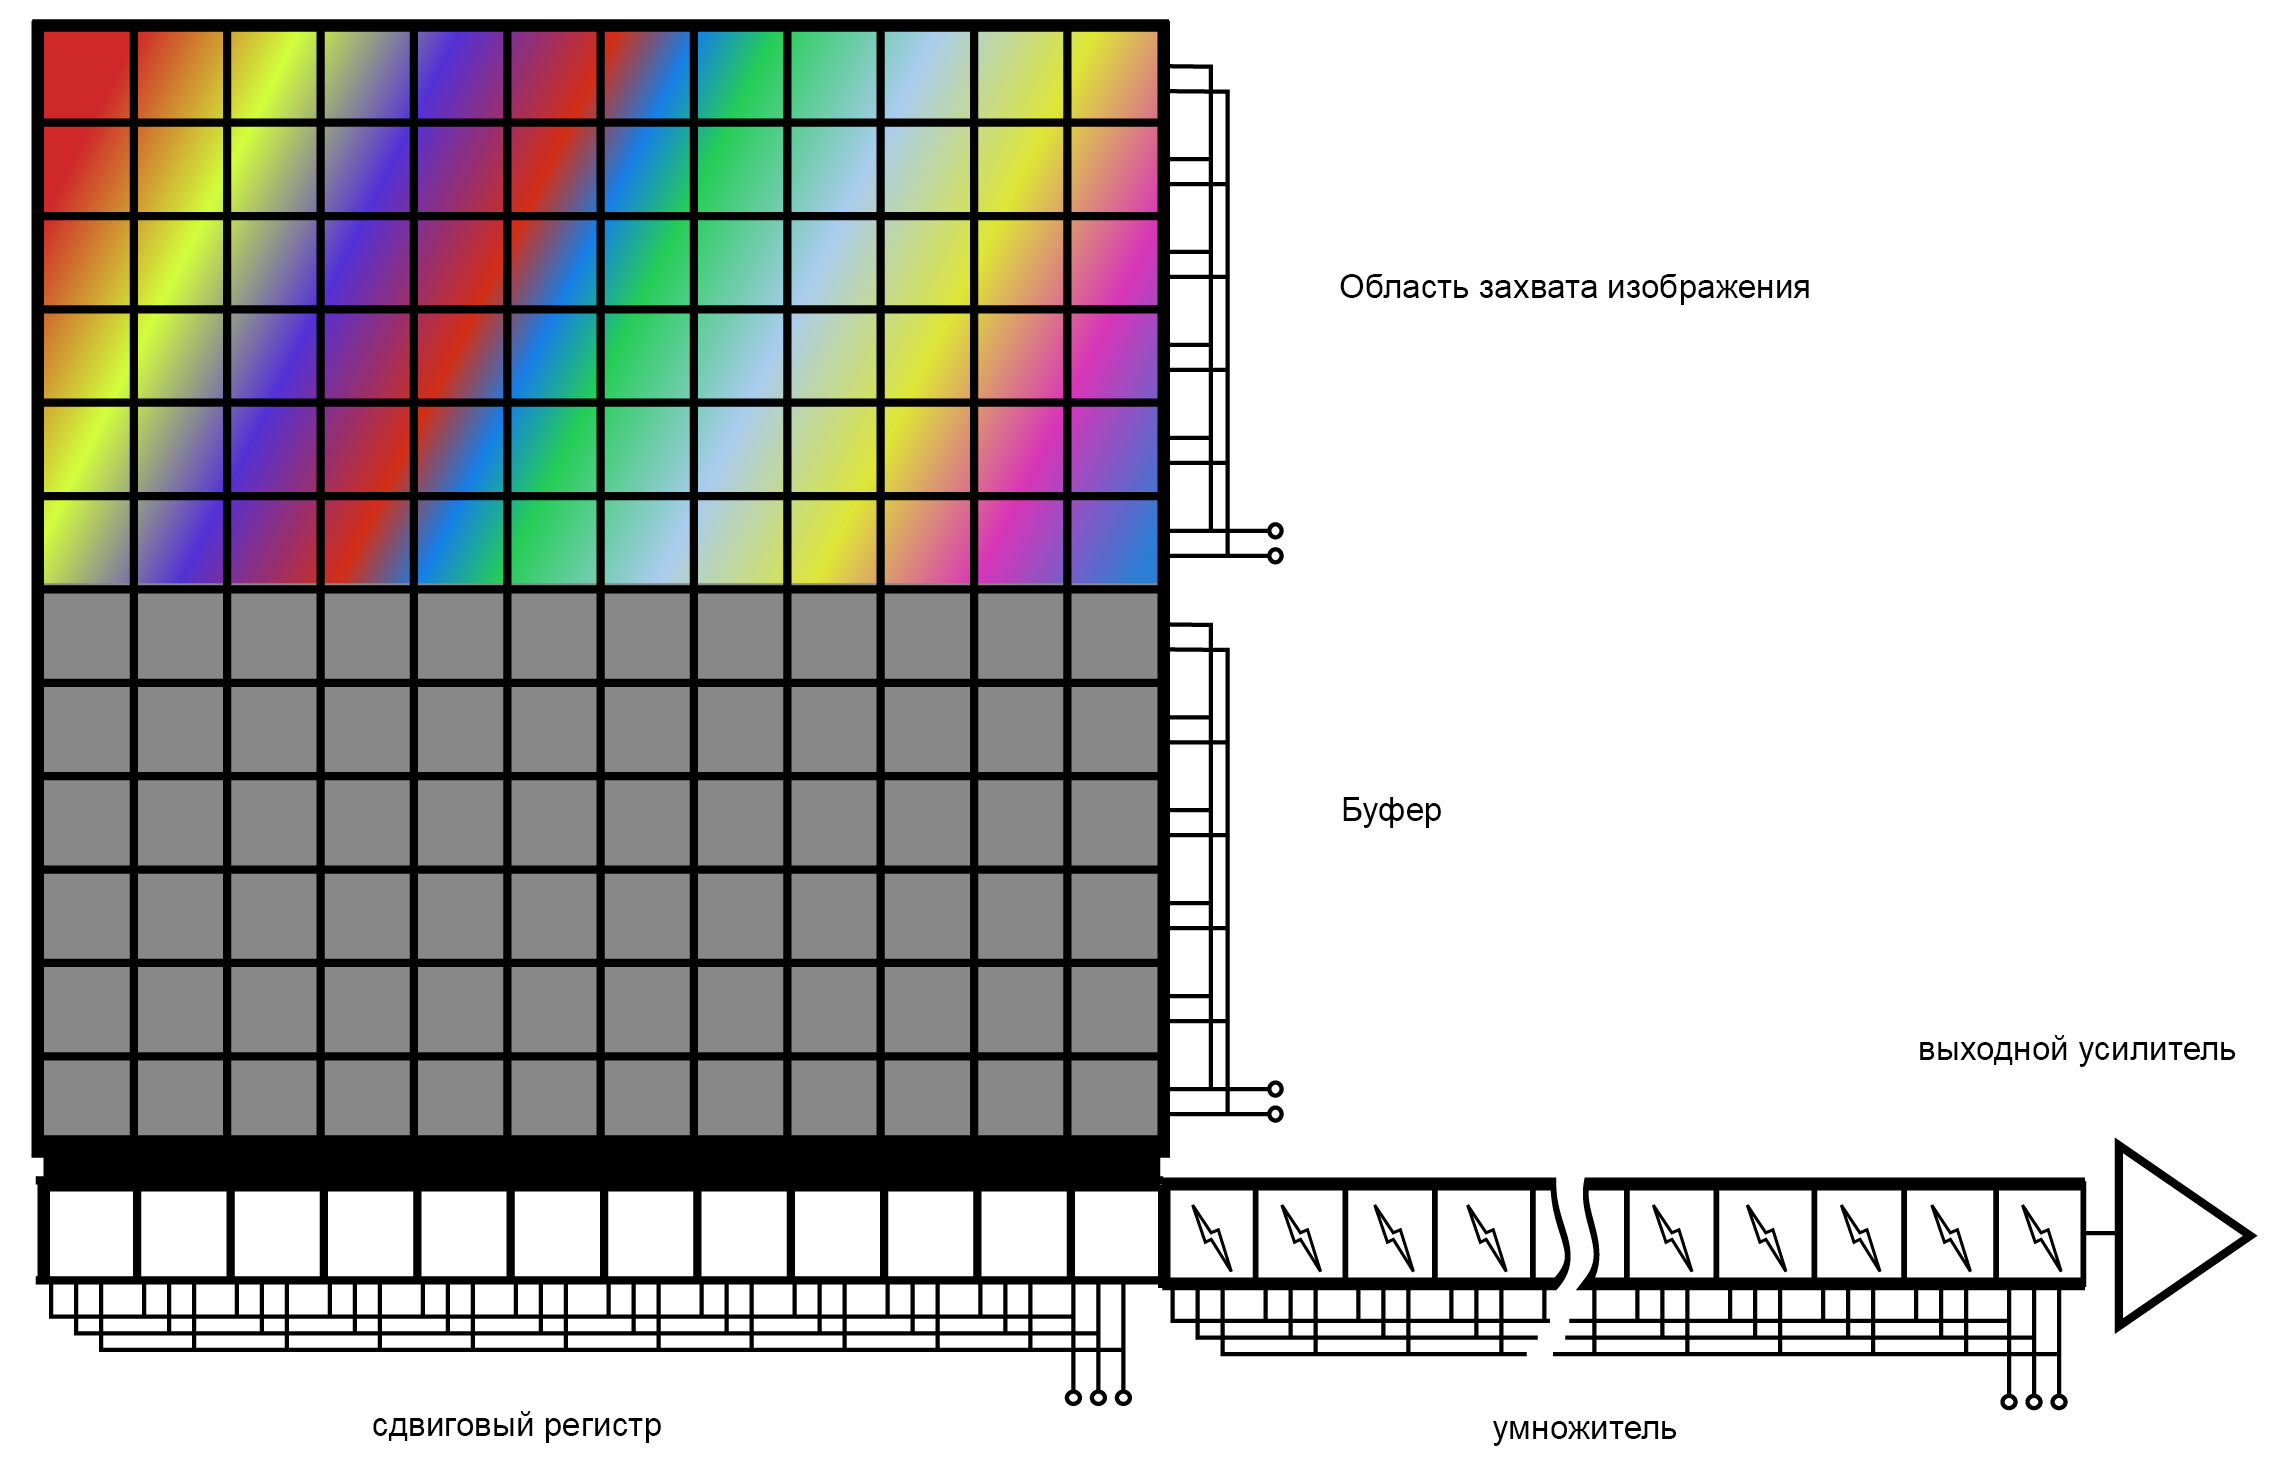
\includegraphics[width=0.7\linewidth]{EMCCD2_color_en} 
		\caption{Позиционно-чувствительный фотодиод \cite[]{CCD2}}
		\label{fig:EMCCD2_color_en}
	\end{figure}
	
\end{itemize}


\section{Выводы по главе} \label{sec:ch1/sec4-}

Бортовые оптико-электронные системы можно разделить на группы:
\begin{itemize}
	\item \textbf{Смотрящего типа}
	
	Характерными требованиями является точность позиционирования. На настоящий момент серийно производимые приборы достигают точности 10 угловых минут.
	
		
	\item \textbf{Излучающие}
	
	Характерным требованием является скорость наведения. На настоящий момент серийно производимые приборы обеспечивают скорости 700 градусов за секунду.
	
	\item \textbf{Мультиплексированные}
	
	Характерным требованием является скорость наведения и точность позиционирования.
	
\end{itemize}

Ниже приведены основные характеристики бортовых оптико-электронных систем: 
\begin{itemize}
\item точность позиционирования \todo{таблица}
\item скорость наведения
\item разрешение 
\item спектральный диапазон
\item частота опроса фотоприемника
\item рабочий сектор
\end{itemize}

Для каждого поколения  \hyperref[acroSOEP]{СОЭП} можно выделить свои особенности:
\begin{itemize}
	\item \textbf{Первого поколения}
	\begin{itemize}
		\item одновременное покрытие всей рабочей полусферы;
		\item простая конструкция;
		\item малая мощность излучения;
		\item малая глубина модуляции;
		\item сильная привязка к типу подавляемой ракеты;
	\end{itemize}
	\item \textbf{Второго поколения}
	\begin{itemize}
		\item большая мощность излучения;
		\item возможность генерации различного типа модуляции;
		\item более сложная конструкция;
		\item малая точность наведения;
		\item большая масса;
	\end{itemize}
	\item \textbf{третьего поколения}
	\begin{itemize}
		\item работоспособность слабо зависит от типа подавляемой ракеты;
		\item использование когерентного излучения;
		\item малая ширина спектра излучения;
		\item большая масса;
		\item большая точнсть наведения.
	\end{itemize}
\end{itemize}

Основными направлениями развития подобных средств противодействия являются:
\begin{itemize}
	\item повышение быстродействия;
	\item использование лазеров, перестраиваемых в широком диапазоне длин волн;
	\item уменьшение размеров и массы;
	\item увеличение энергетического потенциала лазерного излучения;
	\item унификация оборудования (возможность использования на любом типе носителя, возможность согласованного функционирования с различными типами средств ИО и исполнительных средств РЭБ);
	\item модульность конструкции и открытая архитектура.
\end{itemize}
Данная работа направлена на развитие  \hyperref[acroSOEP]{СОЭП}. В главах \ref{ch:ch3}, \ref{ch:ch4} (\nameref{ch:ch3}, \nameref{ch:ch4}) проводятся рассчеты позволяющие повысить быстродействие, точность, уменьшить массу средств противодействия.

Приведены основные способы обеспечения обратной связи в бортовых оптико-электронных системах:
\begin{itemize}
	\item \textbf{по управляющей координате}
	
	При использовании 16 разрядного датчика можно достич точности определения координаты порядка 20 угловых секунд, но на деле точность отработки управляющего воздействия ограничивается точностью исполнительного устройства.
	
	\begin{itemize}
		\item СКВТ (Синусно-косинусный вращающийся трансформатор)
		\item Датчик ХОЛЛА + датчик нуля (оптопара)
		\item Энкодер
	\end{itemize}
		
	\item \textbf{по сигналу с фотоприемника} 
	
	При использовании фотоприемника с частотой опроса 400 Гц и разрешением 512х512 пикселей можно достичь точности сопровождения цели порядка 10 угловых секунд.
	
	\begin{itemize}
		\item Одноэлементные фотоприемники с применением механических модуляторов
		\item Позиционно чувстительные фотоприемники		
		\item Многоэлементные матричные фотоприемники.	
	\end{itemize}
	
	
\end{itemize}
Проведена оценка точности при использовании различных датчиков.Исследование влияния точности и принципа работы датчика проводится в главе \ref{ch:ch5} (\nameref{ch:ch5}).

Кроме оптических характеристик на качество ОЭП в значительной степени влияет время сканирования определенной части пространства, время выхода на заданное целеуказание и точность сопровождения цели. Поэтому при проектировании современных бортовых ОЭП важнейшей задачей является управление направлением линии визирования. Оно осуществляется двумя способами: путем перемещения всего устройства информационных каналов и управлением положением отдельных оптических элементов (зеркал, призм). Применение второго способа обеспечивает высокие динамические и точностные характеристики. \textbf{Этой теме уделяется мало внимания, поэтому далее рассматривается одна из реализаций этого способа.}

Важным этапом разработки любого изделия является создание математической модели, макетирование и моделирование динамики. Распространенной проблемой при разработке изделий является отсутствие методики разработки и исследования динамики систем управления бортовыми оптико-электронными приборами. Применение информационных технологий таких как CAD/CAM средства проектирования, средства математического моделирования (MATHCAD, MatLAB), средства контроля версий позволяют минимизировать человеческий фактор, а следование методике разработки позволяет обеспечить выполнение изначальных требований к проектируемому изделию. Решение вопросов такого характера обсуждается в главе \ref{ch:ch2} (\nameref{ch:ch2}).


\clearpage           % Глава 1
\chapter{Методика разработки и исследования динамики систем управления бортовыми оптико-электронными приборами с применением информационных технологий} \label{ch:ch2}

В настоящее время наиболее распространены в народном хозяйстве и военной технике комплексированные оптико - электронные системы (КОЭП) визуализации, включающие в себя каналы наблюдения и зондирования в широком спектре волн оптического диапазона \cite[]{Tarasov},\cite[]{Belyakov},\cite[]{Karpov},\cite[]{Torshina}. Появление на рынке матричных фотоприемников расширило возможности КОЭП и К(комплексов). Несмотря на интенсивное развитие   теории и методов расчета и совершенствование бортовых автоматических КОЭП и К  возникают ряд вопросов, влияющих на качество получаемой оптической информации, в частности – это вопросы динамики и качества управления и увязки их с оптическими характеристиками каналов визуализации \cite[]{Belyakov},\cite[]{Karpov}, \cite[]{Baloev16}, \cite[]{Karpov17}.

Рассматриваются алгоритмы методики разработки и исследования динамики систем виброзащиты и управления бортовыми оптико- электронными приборами в виде десяти последовательных интерактивных замкнутых процедур от анализа технического задания до испытаний на борту.

Оптико-электронные приборы (ОЭП) авиационного, морского, наземного и космического базирования нашли широкое применение при выполнении задач наблюдения и охраны, в том числе при решении народнохозяйственных задач и задач обороны и безопасности.

В настоящее время широко рекламируются комплексированные ОЭП визуализации, включающие в себя каналы наблюдения и зондирования в широком спектре волн оптического диапазона, для применения в народном хозяйстве и военной технике \cite[]{Tarasov},\cite[]{Belyakov}, \cite[]{Torshina}, \cite[]{Ivanov18}. Появление на рынке матричных фотоприемников расширило возможности ОЭП и комплексов. Несмотря на интенсивное развитие   теории и методов расчета и совершенствование бортовых автоматических ОЭП возникает ряд вопросов, влияющих на качество получаемой оптической информации, в частности – это вопросы динамики и качества управления и увязки их с характеристиками каналов визуализации \cite[]{Tarasov},\cite[]{Belyakov}, \cite[]{Baloev16}, \cite[]{Karpov17}, \cite[]{Gerasin19}. Ниже в развитие работы \cite[]{Tarasov} рассматривается методика разработки и исследования систем автоматического управления (САУ) и виброзащиты (СВ) ОЭП с использованием замкнутых процедур исследования от разработки математических моделей до испытаний на борту носителя.


\section{Методика разработки и исследования динамики} \label{sec:ch2/sec1-}


Разработка СВ и САУ ОЭП начинается с выбора приемлемого варианта. Для этого решается много критерийная задача оптимизации с учетом ряда противоречивых технико-экономических (Т-Э) требований: точность САУ -  $\alpha_{1}$, полосы пропускания САУ и СВ - $\alpha_{21}$, $\alpha_{22}$; качество изображения -  $\alpha_{3}$, время экспозиции -  $\alpha_{4}$ , потребляемая энергия -  $\alpha_{5}$, надежность -  $\alpha_{6}$, масса объекта управления (ОУ) -  $\alpha_{7}$, стоимость -  $\alpha_{8}$, конкурентоспособность - $\alpha_{9}$, характеристики объектива -$\alpha_{10}$ и приемника излучения - $\alpha_{11}$ и т.п., которые определяются из технического задания (ТЗ) на ОЭП методом экспертных оценок специалистов в этих областях науки и техники с учетом предварительных расчетов и исследований. Критерий выбора приемлемого (i) варианта определяется по формуле:

\begin{equation}
\label{eq:p2:1}
\begin{alignedat}{2}
k_i=min\sum_{j=1}^n{\gamma _{ji}\alpha _{ji}}
\end{alignedat}
\end{equation}

где \textit{i} – число вариантов, \textit{n} – число Т-Э параметров, $\gamma_{ij}$ – весовые коэффициенты, $\alpha_{ji}$ – Т-Э параметры. Для выбранных приемлемых вариантов  СВ и САУ (одного или двух) в соответствии с методикой изложенной в главе \ref{ch:ch4} проводится исследование их динамики. За критерий качества САУ обычно принимают совокупность динамических характеристик каналов управления, удовлетворяющих условиям:

\begin{equation}
\label{eq:p2:2}
\begin{alignedat}{2}
\varDelta \alpha _k\leqslant \varDelta \alpha _{k}^{\textit{доп}},
\\
\,\,\,\,\varDelta \dot{\alpha}_k\leqslant \varDelta \dot{\alpha}_{k}^{\textit{доп}},
\\
\,\,\,\,\,\,M\leqslant \text{1.05..1.25,}
\\
\,\,\,\,\left| \left. \varDelta \varphi \right| \right. \geqslant \left( 45-60 \right) ^0,
\\
\,\,\,\,\left| \left. \varDelta L \right|\geqslant \,\,\textit{6дб}, \right. 
\end{alignedat}
\end{equation}

(\ref{eq:p2:1})

где  $\varDelta \alpha^{\textit{доп}}_{k}$, 
$\varDelta \dot{\alpha}^{\textit{доп}}_{k}$, 
$\varDelta \alpha _k$, 
$\varDelta \dot{\alpha}_k$ 
- допустимые установившиеся значения динамических погрешностей САУ и СВ по углу  и угловой скорости  при действии возмущений, полученных в условиях, близких к реальной эксплуатации САУ, \textit{k= 1,2,...} - номер канала управления, обеспечивающего качество изображения, М – показатель колебательности, $\varDelta \varphi$, $\varDelta L$ –запасы устойчивости по фазе и по амплитуде, полученные из логарифмической частотной характеристики  разомкнутой системы \cite[]{Bessekerski20}.

Согласно предлагаемой методике алгоритм разработки СВ, САУ и исследования их динамики представлен в виде 4-х основных последовательных интерактивных замкнутых процедур с использованием 27-ми блоков разработки и исследования (рисунок~\ref{fig:tikz_example}):

\begin{enumerate}
	\item После выполнения последовательных процедур (верификации, разработки расчетной и математической моделей, декомпозиции) с применением компьютерных технологий (Solid Works, MathCAD, MATLAB): (рисунок~\ref{fig:tikz_example}: 1,2,...7) проводится интерактивный синтез алгоритмов управления изолированных каналов САУ частотным методом \cite[]{Bessekerski20} и конструктивных параметров СВ (рисунок~\ref{fig:tikz_example}: 8-9-21-8) до выполнения критериев качества (глава \ref{ch:ch4}). На основании полученной информации проводится разработка и изготовление масштабного динамического макета ОЭП (ОУ, приводов, встроенных датчиков с обеспечением адекватности их динамическим характеристикам) с применением 3Д - принтера (рисунок~\ref{fig:tikz_example}: 10). Далее проводится исследование динамики пространственного движения макета САУ и СВ с использованием синтезированных алгоритмов управления (рисунок~\ref{fig:tikz_example}: 11-12). Если требования ТЗ (рисунок~\ref{fig:tikz_example}: 2) не выполняются, то проводятся последовательно циклы итерационных исследований динамики САУ и СВ : (рисунок~\ref{fig:tikz_example}: 12-20-10,...12), (рисунок~\ref{fig:tikz_example}: 12-20-21-8,...12), (рисунок~\ref{fig:tikz_example}: 12-20-23-3,...12) до обеспечения критериев качества (глава \ref{ch:ch4}), заключающихся в оптимальном выборе параметров регулятора и ОУ.
	\item Далее переходим к исследованию пространственной модели с применением MATLAB: 
	(рисунок~\ref{fig:tikz_example}: 13 – 14 - 15). Если критерии (глава \ref{ch:ch4}) не выполняются, то переходим на 2-е круги последовательных итераций: (рисунок~\ref{fig:tikz_example}: 15-24-21-8,...15), (рисунок~\ref{fig:tikz_example}: 15-24-23-3,...15), где доопределяем число степеней свободы математической модели и её параметры, параметры САУ и СВ путем последовательных предыдущих итераций исследований до выполнения критериев (глава \ref{ch:ch4}). C учетом полученной информации доопределяем: необходимые конструктивные доработки  ОУ, САУ, СВ ; приемлемые варианты построения СВ и САУ, а также в случае необходимости уточняем критерии (глава \ref{ch:ch4}) и задачи, которые могут решать СВ и САУ, а также ограничения и нелинейности в контурах управления. По результатам исследования делается заключение о необходимости изготовления опытного образца САУ и СВ или проведения дальнейших исследований.
	
	\item Затем переходим к испытаниям опытного образца САУ и СВ на стендах в соответствии с методиками испытаний и требований ТЗ: (рисунок~\ref{fig:tikz_example}: 16-17). Если критерии (глава \ref{ch:ch4}) не выполняются, то переходим  на 
	3-и круги последовательных итерационных процедур: (рисунок~\ref{fig:tikz_example}: 17-25-21-8,...17), (рисунок~\ref{fig:tikz_example}: 17-25-26-1,...17), которые включает в себя две предыдущих. Результаты исследований фиксируют в протоколе испытаний и делают заключение о необходимости доработок СВ и САУ или допуске их к испытаниям на борту. 
	
	\item В заключении переходим к испытаниям САУ и СВ на борту в соответствии с методиками натурных испытаний и требований ТЗ: (рисунок~\ref{fig:tikz_example}: 18-19). Если критерии (глава \ref{ch:ch4}) не выполняются, то переходим  на 
	4-и круги последовательных итерационных процедур: (рисунок~\ref{fig:tikz_example}: 19-27-23-3,...19), (рисунок~\ref{fig:tikz_example}: 19-27-26-1,...19), которые включают в себя (при необходимости) три предыдущие. Результаты испытаний и требования к техническим характеристикам СВ и САУ фиксируем в протоколе испытаний и делаем заключение о необходимости доработок СВ и САУ или допуске их к дальнейшему производству.
	Приведенная методика была апробирована при разработке ряда САУ ОЭП \cite[]{Belyakov}, \cite[]{Karpov}, \cite[]{Baloev16}, \cite[]{Karpov17}, \cite[]{Gerasin19}, \cite[]{Molin21}. Каждому из блоков на рисунке ниже (рисунок~\ref{fig:tikz_example}) присущи своя специфика и его математическое или логическое описание и предполагается соответствующая методика его разработки. Некоторые из них приводятся ниже.

\end{enumerate}

\section{Оценка допуска на точность стабилизации изображения} \cite[]{Belyakov}, \cite[]{Sokolski22}, \cite[]{Molin21} \label{sec:ch2/sec2} 



Для изучения процесса формирования изображения с учетом множества факторов, влияющих на формирование, преобразование и передачу качества изображения, рассмотрим функциональную схему одного из вариантов комплексированного ОЭП (рисунок~\ref{fig:oep_sch}), представляющего собой совокупность \hyperref[acroTVS]{тепловизионной системы (ТВС)}, \hyperref[acroTS]{телевизионной системы (ТС)}, фотографической системы (ФС), наблюдательных приборов в видимой и ближней инфракрасной (ИК) областях. В результате действия внешних возмущений $F(P,g,T,t)$, возмущений, идущих от носителя, и наличия управления ОЭП в пространстве остается не компенсированный сдвиг изображения (динамическая погрешность).


\begin{figure}[ht]
	{\centering
		\ifdefmacro{\tikzsetnextfilename}{\tikzsetnextfilename{tikz_example_compiled}}{}% присваиваемое предкомпилированному pdf имя файла
		% !TEX encoding = UTF-8 Unicode
% Úτƒ-8 encoded
% http://www.linux.org.ru/forum/general/10357036
\tikzset{
    line/.style={draw, -latex'},
    every join/.style={line},
    u/.style={anchor=south},
    r/.style={anchor=west},
    fxd/.style={text width = 6em},
    it/.style={font={\small\itshape}},
    bf/.style={font={\small\bfseries}}
}
\tikzstyle{base} =
    [
        draw,
        on chain,
        on grid,
        align=center,
        minimum height=4ex,
        minimum width = 10ex,
        node distance = 6mm and 60mm,
        text badly centered
    ]
\tikzstyle{coord} =
    [
        coordinate,
        on chain,
        on grid
    ]
\tikzstyle{cloud} =
    [
        base,
        ellipse,
        fill = red!5,
        node distance = 3cm,
        minimum height = 2em
    ]
\tikzstyle{decision} =
    [
        base,
        diamond,
        aspect=2,
        fill = green!10,
        node distance = 2cm,
        inner sep = 0pt
    ]
\tikzstyle{block} =
    [
        rectangle,
        base,
        fill = blue!3,
        rounded corners,
        minimum height = 2em
    ]
\tikzstyle{print_block} =
    [
        base,
        tape,
        tape bend top=none,
        fill = yellow!10
    ]
\tikzstyle{io} =
    [
        base,
        trapezium,
        trapezium left angle = 70,
        trapezium right angle = 110,
        fill = blue!5
    ]
\makeatletter
\pgfkeys{/pgf/.cd,
    subrtshape w/.initial=2mm,
    cycleshape w/.initial=2mm
}
\pgfdeclareshape{subrtshape}{
    \inheritsavedanchors[from=rectangle]
    \inheritanchorborder[from=rectangle]
    \inheritanchor[from=rectangle]{north}
    \inheritanchor[from=rectangle]{center}
    \inheritanchor[from=rectangle]{west}
    \inheritanchor[from=rectangle]{east}
    \inheritanchor[from=rectangle]{mid}
    \inheritanchor[from=rectangle]{base}
    \inheritanchor[from=rectangle]{south}
    \backgroundpath{
        \southwest \pgf@xa=\pgf@x \pgf@ya=\pgf@y
        \northeast \pgf@xb=\pgf@x \pgf@yb=\pgf@y
        \pgfmathsetlength\pgfutil@tempdima{\pgfkeysvalueof{/pgf/subrtshape w}}
        \def\ppd@offset{\pgfpoint{\pgfutil@tempdima}{0ex}}
        \def\ppd@offsetm{\pgfpoint{-\pgfutil@tempdima}{0ex}}
        \pgfpathmoveto{\pgfqpoint{\pgf@xa}{\pgf@ya}}
        \pgfpathlineto{\pgfqpoint{\pgf@xb}{\pgf@ya}}
        \pgfpathlineto{\pgfqpoint{\pgf@xb}{\pgf@yb}}
        \pgfpathlineto{\pgfqpoint{\pgf@xa}{\pgf@yb}}
        \pgfpathclose
        \pgfpathmoveto{\pgfpointadd{\pgfpoint{\pgf@xa}{\pgf@yb}}{\ppd@offsetm}}
        \pgfpathlineto{\pgfpointadd{\pgfpoint{\pgf@xa}{\pgf@ya}}{\ppd@offsetm}}
        \pgfpathlineto{\pgfpointadd{\pgfpoint{\pgf@xb}{\pgf@ya}}{\ppd@offset}}
        \pgfpathlineto{\pgfpointadd{\pgfpoint{\pgf@xb}{\pgf@yb}}{\ppd@offset}}
        \pgfpathclose
    }
}
\pgfdeclareshape{cyclebegshape}{
    \inheritsavedanchors[from=rectangle]
    \inheritanchorborder[from=rectangle]
    \inheritanchor[from=rectangle]{north}
    \inheritanchor[from=rectangle]{center}
    \inheritanchor[from=rectangle]{west}
    \inheritanchor[from=rectangle]{east}
    \inheritanchor[from=rectangle]{mid}
    \inheritanchor[from=rectangle]{base}
    \inheritanchor[from=rectangle]{south}
    \backgroundpath{
        \southwest \pgf@xa=\pgf@x \pgf@ya=\pgf@y
        \northeast \pgf@xb=\pgf@x \pgf@yb=\pgf@y
        \pgfmathsetlength\pgfutil@tempdima{\pgfkeysvalueof{/pgf/cycleshape w}}
        \pgfpathmoveto{\pgfqpoint{\pgf@xa}{\pgf@ya}}
\pgfpathlineto{\pgfpointadd{\pgfpoint{\pgf@xa}{\pgf@yb}}{\pgfpoint{0ex}{-\pgfutil@tempdima}}}
\pgfpathlineto{\pgfpointadd{\pgfpoint{\pgf@xa}{\pgf@yb}}{\pgfpoint{\pgfutil@tempdima}{0ex}}}
\pgfpathlineto{\pgfpointadd{\pgfpoint{\pgf@xb}{\pgf@yb}}{\pgfpoint{-\pgfutil@tempdima}{0ex}}}
\pgfpathlineto{\pgfpointadd{\pgfpoint{\pgf@xb}{\pgf@yb}}{\pgfpoint{0ex}{-\pgfutil@tempdima}}}
\pgfpathlineto{\pgfqpoint{\pgf@xb}{\pgf@ya}}
        \pgfpathclose
    }
}
\pgfdeclareshape{cycleendshape}{
    \inheritsavedanchors[from=rectangle]
    \inheritanchorborder[from=rectangle]
    \inheritanchor[from=rectangle]{north}
    \inheritanchor[from=rectangle]{center}
    \inheritanchor[from=rectangle]{west}
    \inheritanchor[from=rectangle]{east}
    \inheritanchor[from=rectangle]{mid}
    \inheritanchor[from=rectangle]{base}
    \inheritanchor[from=rectangle]{south}
    \backgroundpath{
        \southwest \pgf@xa=\pgf@x \pgf@ya=\pgf@y
        \northeast \pgf@xb=\pgf@x \pgf@yb=\pgf@y
        \pgfmathsetlength\pgfutil@tempdima{\pgfkeysvalueof{/pgf/cycleshape w}}
        \pgfpathmoveto{\pgfqpoint{\pgf@xb}{\pgf@yb}}
\pgfpathlineto{\pgfpointadd{\pgfpoint{\pgf@xb}{\pgf@ya}}{\pgfpoint{0ex}{\pgfutil@tempdima}}}
\pgfpathlineto{\pgfpointadd{\pgfpoint{\pgf@xb}{\pgf@ya}}{\pgfpoint{-\pgfutil@tempdima}{0ex}}}
\pgfpathlineto{\pgfpointadd{\pgfpoint{\pgf@xa}{\pgf@ya}}{\pgfpoint{\pgfutil@tempdima}{0ex}}}
\pgfpathlineto{\pgfpointadd{\pgfpoint{\pgf@xa}{\pgf@ya}}{\pgfpoint{0ex}{\pgfutil@tempdima}}}
\pgfpathlineto{\pgfqpoint{\pgf@xa}{\pgf@yb}}
        \pgfpathclose
    }
}
\makeatother
\tikzstyle{subroutine} =
    [
        base,
        subrtshape,
        fill = green!25
    ]
\tikzstyle{cyclebegin} =
    [
        base,
        cyclebegshape,
        fill = blue!25
    ]
\tikzstyle{cycleend} =
    [
        base,
        cycleendshape,
        fill = blue!25
    ]
\tikzstyle{connector} =
    [
        base,
        circle,
        fill = red!25
    ]

\begin{tikzpicture}[%
    start chain=going below,    % General flow is top-to-bottom
    node distance=6mm and 150mm, % Global setup of box spacing
        ]
        \node [cloud] (start) {Начало};
        \node [block, join] (phase1) {1,2};
        \node [block, join] (phase3) {3};
        \node [block, join] (phase4) {4567};
        \node [block, join] (phase8) {8};
        \node [block, join] (phase9) {9};
        \node [block, join] (phase10) {10};
        \node [block, join] (phase11) {11};
        \node [decision, join, right of = phase11, node distance = 4cm] (condition12) {12};
        \node [block, join, left of = condition12, node distance = 4cm] (phase13) {13,14};
        \node [decision, join, right of = phase13, node distance = 4cm] (condition15) {15};
        \node [block, join, left of = condition15, node distance = 4cm] (phase16) {16};
        \node [decision, join, right of = phase16, node distance = 4cm] (condition17) {17};
        \node [block, join, left of = condition17, node distance = 4cm] (phase18) {18};
        \node [decision, right of = phase18, node distance = 4cm] (condition19) {19};
        \node [cloud] (fin) {Конец};
        
        \node [block, right of = phase1, node distance = 4cm] (print26) {26};
        \node [block, right of = phase3, node distance = 4cm] (print23) {23};
        \node [block, right of = phase8, node distance = 4cm] (print21) {21};
        \node [decision, right of = condition12, node distance = 4cm] (print20) {20};
        \node [decision, right of = condition15, node distance = 4cm] (print24) {24};
        \node [decision, right of = condition17, node distance = 4cm] (print25) {25};
        \node [decision, right of = condition19, node distance = 4cm] (print27) {27};
        
        \path [line, red] (condition12) -| node [u,near start] {Нет} (print20);
        \path [line, red] (condition15) -| node [u,near start] {Нет} (print24);
        \path [line, red] (condition17) -| node [u,near start] {Нет} (print25);
        \path [line, red] (condition19) -| node [u,near start] {Нет} (print27);
        
        \path [line, green] (condition19) to node [r] {Да}(fin);
        
        \node [cyclebegin] (phase2) {Этап 2};
        \node [block, join=by green] (phase3) {Этап 3};
        \node [cycleend, join] (phase4) {Этап 4};
        \node [subroutine, join, subrtshape w = 3mm, fxd] (phase5) {Этап 5 1 2 3 4 5 6 7 8 9 0};
        \node [io, join, fxd] (input) {Этап 6 "--- ввод данных};
        \node [block, join] (phase7) {Этап 7};
        \node [decision, join] (condition) {Условие};
        \node [connector] (finish) {Конец};
        \node [block, left of = phase4, node distance = 4cm] (correction) {Коррекция};
        \node [print_block, right of = phase4, node distance = 4cm] (print) {Print};
        \path [line, red] (condition) -| node [u,near start] {Нет} (correction);
        \path [line] (correction) |- (phase1);
        \path [line] (phase2) -| node [r,near end] {Печать} (print);
        \path [line, green] (condition) to node [r] {Да}(finish);
\end{tikzpicture}

		
	}
	\legend{}
	\caption[Пример \texttt{tikz} схемы]{Пример рисунка, рассчитываемого
		\texttt{tikz}, который может быть предкомпилирован}
	\label{fig:tikz_example}
\end{figure}


Это приводит к изменению структуры изображения аналогично влиянию аберраций, т.е. к ухудшению качества изображения, зависящего от величины и характера изменения динамических погрешностей управляющих систем. Для оценки допуска на точность стабилизации изображения используют частотный критерий качества изображения ОЭП – функцию передачи модуляции (ФПМ) [12].

\begin{figure}[ht]
	\centering
	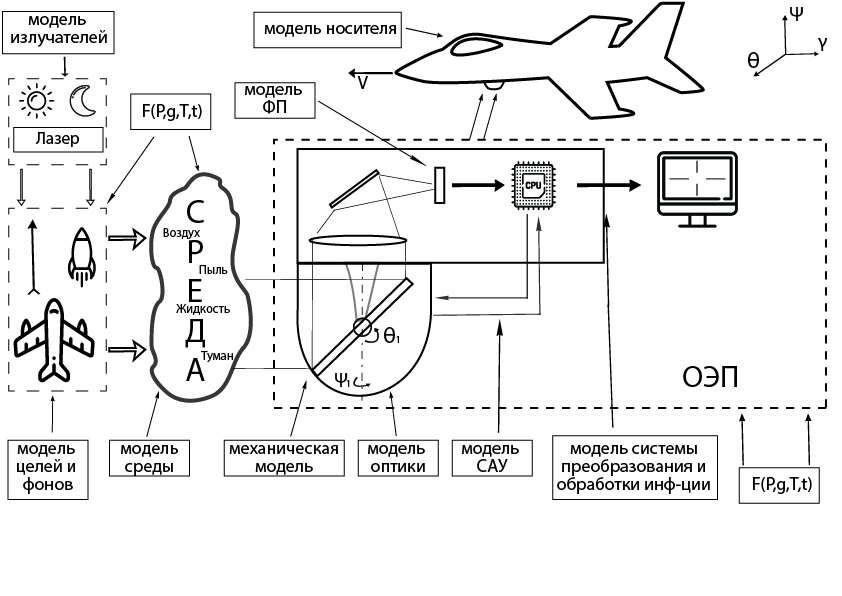
\includegraphics[width=0.8\linewidth]{oep_sch} 
	\caption{Функциональная схема обобщённой модели ОЭП}
	\label{fig:oep_sch}
\end{figure}


\section{Разработка математической модели} \label{sec:ch2/sec3}

\section{Верификация параметров} \label{sec:ch2/sec4}

\section{Оценки декомпозируемости каналов управления, основанные на анализе устойчивости и качества регулирования каналов управления с учетом перекрестных связей в частотной области} \label{sec:ch2/sec5}

\section{Синтез регуляторов частотным методом} \label{sec:ch2/sec6}

\section{Разработка КИМ и исследование динамики пространственной модели} \label{sec:ch2/sec7}

\section{Разработка алгоритмов управления БОЭП} \label{sec:ch2/sec8}

\section{Разработка компьютерной имитационной модели} \label{sec:ch2/sec9}

\section{Макетные испытания} \label{sec:ch2/sec10}

\section{Выводы по главе} \label{sec:ch2/sec11}



ll
           % Глава 2
\chapter{Математическая модель БОЭП как объекта управления} \label{ch:ch3}

\section{Принципиальная схема} \label{ch:ch3/sect1}

\section{Механическая модель} \label{ch:ch3/sect1}

\subsection{Основные допущения, системы координат} \label{sec:ch2/sec1}

\subsection{Геометрия масс} \label{sec:ch2/sec1}

\section{Составление уравнений динамической модели ОУ} \label{ch:ch3/sect1}


\subsection{Вычисление кинетической энергии} \label{sec:ch2/sec1}

\subsection{Вычисление обобщенных сил} \label{sec:ch2/sec1}

\subsection{Составление уравнений динамической модели ОУ} \label{sec:ch2/sec1}


\section{Модель привода} \label{ch:ch3/sect1}

\section{Линеаризованная система} \label{ch:ch3/sect1}

\section{Выводы по главе} \label{ch:ch3/sect1}


Некоторый текст.

\clearpage           % Глава 3
\chapter{Разработка алгоритмов управления БОЭП} \label{ch:ch4}

Объектом исследования является системы автоматического управления (САУ) оптико-электронным прибором (ОЭП) в пространстве по азимуту и углу места в режимах наведения и стабилизации.

Цель работы – является разработка компьютерной имитационных моделей изолированных каналов управления ОЭП, управляемого моментными двигателями по азимуту и углу места и исследование его динамических свойств.
В процессе работы проводились выбор моментных двигателей, синтез алгоритмов управления, разработка компьютерных имитационных моделей изолированных нелинейных каналов управления бортового ОЭП и исследование динамики управления им в режимах наведения и стабилизации.

В результате исследования динамики предложены алгоритмы управления и требования к структуре и элементам изолированных каналов управления, обеспечивающие требования ТЗ, которые будут уточнены при исследовании пространственной задачи управления.

Эффективность управления в режиме наведения достигается применением оптимального управления по быстродействию. 
Все расширяющийся круг военных и гражданских задач, для решения которых широко используются оптико-электронные методы и средства, вызвало интерес к решению научно- технических   проблем, возникающих при решении этих задач \cite[]{Tarasov}, \cite[]{Fedoseev}.

Одна из важных проблем – это влияние динамики и управления на достижение требуемых тактико- технических характеристик бортовых ОЭП и комплексов. Вопросы разработки, моделирования и исследования динамических систем, в том числе бортовых оптико-электронных комплексов, отражены в трудах международных Четаевских конференций по аналитической механике, устойчивости и управлению; в трудах международных симпозиумов по автоматическому управлению и всесоюзных совещаниях по теории инвариантности, в трудах КАИ, а также в журналах: «Оптический журнал», «Гироскопия и навигация», «Оптико-механическая промышленность», «Автоматика и телемеханика», «Авиационная техника», «Вестник КГТУ им. А. Н. Туполева» [4-26]. Разработке алгоритмов и исследованию динамики, и управлению посвящены работы [3 - 29].

На данном этапе разработки выполняемой НИР проведены предварительные расчеты по уяснению решаемых задач и анализу исходных данных, оговоренных техническим заданием (ТЗ), разработке и согласованию
расчетных оптико – механической схем и параметров ОЭП, приводов, датчиков угла САУ с учетом их технических требований и внешних воздействий от носителя.


\section{Технические требования и режимы управления ОЭП} \label{ch:ch4/sect1}

В соответствии с требованиями ТЗ были проанализированы, уточнены, доопределены следующие исходные данные, необходимые для расчета:
\begin{itemize}
	\item Состав системы автоматического управления,
	\item САУ по азимуту,
	\item САУ по углу места,
	\item Датчики углового положения по азимуту и углу места,
	\item Двигатели типа ДБМ (уточняются в процессе разработки) по азимуту и углу места,
	\item Усилительно-преобразовательные блоки каналов управления совместно с микропроцессорными блоками,
	\item Назначение и технические требования.
\end{itemize}
САУ предназначена для наведения оси визирования на заданные угловые координаты относительно строительных осей летательного аппарата (ЛА), параметры движения ЛА.

\newpage
%%%%%%%%%%%%%%%%%%%% Table No: 9 starts here %%%%%%%%%%%%%%%%%%%%

\begin{table}[!h]
	\caption{Технические параметры САУ}%
	\label{tab:SAU_PARAM}% label всегда желательно идти после caption
	\begin{longtable}{|m{5cm}|m{5.5cm}|m{5.5cm}|}
		\hline
		& по азимуту & по углу места \\ 
\hline
Пределы наведения		& $\pm$ 180 град           & (-60 .. +30) град              \\ 
\hline
Максимальная скорость наведения		&600 град/сек            &300 град/сек               \\ 
		\hline
Максимальная среднеквадратическая погрешность наведения и стабилизации		&<30 угловых минут           &<30 угловых минут               \\ 
		\hline
Время наведения на предельный угол		&<0.6 с            & <0.6 с              \\ 
		\hline
Синусоидальные вибрации		& \multicolumn{2}{m{11cm}|}{
	\begin{tabular}[l]{m{11cm}}
		Частота 5-10 Гц, амплитуда перемещения 5 мм\\
		Частота 20-22 Гц, ускорение $25 \textit{м/с}^2$\\
		Частота 35,4-50 Гц, амплитуда перемещения 0.5 мм\\
		Частота 50-500 Гц, ускорение $25 \textit{м/с}^2$
	\end{tabular}

}      \\ 
		\hline
Требования к САУ при внешних воздействиях		& \multicolumn{2}{m{11cm}|}{\begin{tabular}[l]{m{11cm}}
		максимальной скорости движения носителя – 56 м/с (200км/час)\\
		максимальный крен ЛА $\leq 15^0$\\
		угловая скорость носителя $\omega_y=12$ град/c\\
		минимальная высота полета носителя – 1500 м\\
		максимальная скорость движения ОН – 500 м/с	
\end{tabular}}      \\ 
		\hline
Гармонические возмущения, идущие от ЛА по азимуту и углу места		& \multicolumn{2}{m{11cm}|}{\begin{tabular}[l]{m{11cm}}
		Частота 0.16 Гц, амплитуда колебаний 12 град.\\
		Частота 1 Гц, амплитуда колебаний 1- 2 град.
\end{tabular}}      \\ 
		\hline
Требования к САУ при воздействиях ускорений в условиях движения носителя		& \multicolumn{2}{m{11cm}|}{$4.8 \textit{м/с}^2$}      \\ 
		\hline
	\end{longtable}
\end{table}

%%%%%%%%%%%%%%%%%%%% Table No: 9 ends here %%%%%%%%%%%%%%%%%%%%

Геометрия масс тел вращения объекта управления (ОУ) по двум осям управления опредставлена в таблице \ref{tab:MASS/3.1} и рисунокe \ref{fig:41}.

%%%%%%%%%%%%%%%%%%%% Figure/Image No: 30 starts here %%%%%%%%%%%%%%%%%%%%

\begin{figure}[!ht]
	\centering
	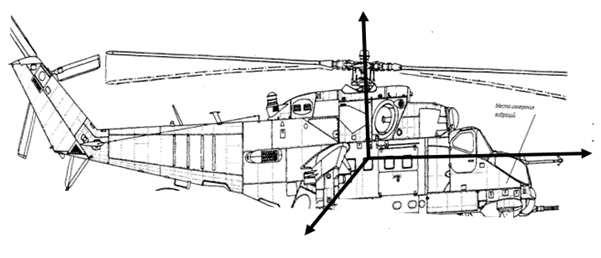
\includegraphics[width=0.8\linewidth]{img-25} 
	\caption{Обозначение строительных осей ЛА}
	\label{fig:41}
\end{figure}

%%%%%%%%%%%%%%%%%%%% Figure/Image No: 30 Ends here %%%%%%%%%%%%%%%%%%%%

В отчете приведены синтез алгоритмов управления, разработка компьютерных моделей и исследование динамики изолированных каналов управления САУ с учетом частоты ШИМ и насыщения усилителей мощности, дискретизации датчиков угла.


\section{Обоснование выбора приводов} \label{ch:ch4/sect2}

Требуемая мощность и развиваемый момент двигателя определяются по формулам \cite[]{Bessekerski}:\par


\begin{equation}
	\label{eq:p4:1}
	\begin{multlined}
P \geq 2 \left( M_{\textit{нагр}}+I_{\textit{нагр}} \ddot \alpha^{max}   \right) \dot \alpha^{max},\\
M_{\textit{дв}} \geq 2 \left[ M_{\textit{нагр}}+I_{\textit{нагр}} \ddot \alpha^{max}  \right], \\
M_{\textit{нагр}}=M_{\textit{тр}}+M_{\textit{дб}}.
\end{multlined}
\end{equation}

Здесь 
$P$ - мощность двигателя, 
$М_{\textit{дв}}$ – момент на валу двигателя, 
$M_{\textit{нагр}}$ - статический момент нагрузки, 
$I_{\textit{нагр}}$ - момент  инерции нагрузки, 
$М_{\textit{тр}}$ - момент трения на валу двигателя,
$М_{\textit{дб}}$ - момент дисбаланса нагрузки,  
$\ddot \alpha^{max}, \dot \alpha^{max}$ - максимальные угловые скорость и ускорение.\par

Оценим указанные параметры двигателей. 
В соответствии с требованиями ТЗ следует, что наиболее энергоемким является режим наведения. Ставится задача перевода оптической оси ОЭП относительно строительных осей ЛА за время \textit{0.6 с}. из одного положения в другое в пределах углов: по азимуту – $2 \alpha_0 = 360$ град., по углу места – $2 \beta_0 = 90$ град.  \par

Для решения этой задачи рассмотрим оптимальное управление по быстродействию (по минимуму времени перевода оптической оси ОЭП из одной точки пространства в другую) \cite[]{Babaev},\cite[]{Boltanski}. Суть такого управления состоит в том, что для перевода оптической оси на требуемый угол за минимальное время необходимо в первой половине этого времени разгоняться с постоянным положительным ускорением, а в другой половине – тормозить с постоянным отрицательным ускорением. Таким образом изменение угла поворота ОЭП будет проходить по нелинейной траектории (двум параболам).\par

Требуемое угловые ускорение и скорость ротора моментного двигателя с нагрузкой по азимуту, необходимое для достижения необходимого половинного угла $2 \beta_0 = 45$ град. за время $\tau=0.3$ с:\par

\begin{equation}
\label{eq:p4:1+}
\begin{multlined}
  \alpha _{0} = \frac{ \ddot \alpha _{0} \tau^{2}}{2} \rightarrow 
\ddot \alpha _{0} = \frac{2 \alpha _{0}}{ \tau^{2}} = \frac{2 \pi /2}{  0.3^{2}} = 34.906 \textit{рад/с}^{2},\\
\dot \alpha ^{max}= \ddot \alpha _{0} \tau = 34.906\cdot 0.3=10.47 \textit{рад/с}. 
\end{multlined}
\end{equation}

Требуемое угловые ускорение и скорость ротора моментного двигателя с нагрузкой по углу места, необходимое для достижения необходимого половинного угла $\beta_0=45$ град. за время $\tau=0.3$ с:

\begin{equation}
\label{eq:p4:1+1}
\begin{multlined}
\beta _{0} = \frac{ \ddot \beta _{0} \tau^{2}}{2} \rightarrow 
\ddot \beta _{0} = \frac{2 \beta _{0}}{ \tau^{2}} = \frac{2 \pi /4}{  0.3^{2}} = 17.453 \textit{рад/с}^{2},\\
\dot \beta ^{max}= \ddot \beta _{0} \tau = 17.453\cdot 0.3=5.235 \textit{рад/с}. 
\end{multlined}
\end{equation}
Моменты трения оценим по формуле:

\begin{equation}%\tag{44}
\label{eq:p4:4}
\begin{multlined}
	M_{\textit{тр}}= \left( 2  \div 5 \right) m 10^{-3} \left[ \textit{Нм} \right] 
\end{multlined}
\end{equation}
где \textit{m} – масса подвижной части прибора. С учетом данных из таблицы \ref{tab:MASS/3.1} (m1=15.7 кг, m2=1.131 кг) находим по формуле 41):\par

\begin{equation}%\tag{44}
\label{eq:p4:4+}
\begin{multlined}
M_{\textit{ТР1}} = 5 \cdot 10^{-3}\cdot 15.7 = 0.0785 \textit{Нм},\\
M_{\textit{ТР2}} = 5 \cdot 10^{-3}\cdot 1.131 = 0.005755 \textit{Нм}
\end{multlined}
\end{equation}

Моменты дисбаланса нагрузки определим по формулам:
\begin{equation}%\tag{44}
\label{eq:p4:4+1}
\begin{multlined}
M_{\textit{дб1}} = 
m_{1} \left( a+g \right) \sqrt[]{x_{c1}^{2}+y_{c1}^{2}} =
15.7 \left( 4.8 + 9.8 \right) \cdot 9 \cdot 10^{-3}=2.06 \textit{Нм},\\
M_{\textit{дб2}}=
m_{2} \left( a+g \right) y_{c2}=
1.131 \cdot 14.8 \cdot 10^{-3} = 0.245 \textit{Нм},
\end{multlined}
\end{equation}

здесь \textit{а }– ускорение, создаваемое носителем, \textit{g} – ускорение земного притяжения, \textit{х\textsubscript{с1},у\textsubscript{с1},у\textsubscript{с2}} – величины дисбаланса ОЭП (таблица \ref{tab:MASS/3.1})\par

Максимальные статические моменты нагрузки на валу двигателей по азимуту и углу места соответственно равны:\par

\begin{equation}%\tag{44}
\label{eq:p4:4+2}
\begin{multlined}
M_{\textit{нагр1}}=M_{\textit{ТР1}}+M_{\textit{дб1}}=0.078+2.064=2.1425 \textit{Нм}, \\
M_{\textit{нагр2}}=0.005755+0.245=0.250755 \textit{Нм}.
\end{multlined}
\end{equation}

В результате получили следующие исходные данные для расчета требуемых моментов и мощностей на валу двигателей:\par


	\begin{tabular}{ll}
\( \ddot \alpha _{0}=34,9\textit{рад/с}^{2} \)				& \( \ddot \beta _{0}=17.45 \textit{рад/с}^{2} \)  \\
\( I_{y}=0.327\textit{кгм}^{2} \)						&  \( I_{z}=0.0084 \textit{кгм}^{2} \) \\
\( m_{1}=15.7\textit{кг} \)								& \( m_{2}=1.131 \textit{кг} \) \\
\( \dot \alpha ^{max}=10.47\textit{рад/с} \)				& \( \dot \beta ^{max}=5.235\textit{рад/с} \) \\
\( M_{\textit{\textit{нагр1}}}=2.1425\textit{Нм} \)		& \( M_{\textit{\textit{нагр2}}}=0.250755\textit{Нм} \)
	\end{tabular}


В силу (\labelcref{eq:p4:1}) получим требования к двигателям по азимуту и углу места:\par

- к пусковому моменту на валу ротора

\begin{equation}%\tag{44}
\label{eq:p4:4+3}
\begin{multlined}
M_{\textit{дв1}} \geq 2 \left[ 2.1425 + \left( 0.327 \cdot 34.9 \right)  \right] =27.1096\textit{Нм} \rightarrow 30\textit{Нм}, \\
M_{\textit{дв2}} \geq 2 \left[ 0.25 + 0.0084 \cdot 17.45 \right] =0.79316\textit{Нм} \rightarrow 1\textit{Нм};
\end{multlined}
\end{equation}

- к потребляемой мощности

\begin{equation}%\tag{44}
\label{eq:p4:4+4}
\begin{multlined}
P_{1}=27.11 \cdot 10.47=283.84\textit{Вт} \rightarrow 300\textit{Вт}, \\
P_{2}=0.8 \cdot 5.235=4.2\textit{Вт} \rightarrow  \left( 5 \div 10 \right) \textit{Вт}.
\end{multlined}
\end{equation}
С учетом полученных требований можно использовать наиболее приемлемые моментные двигатели (МД) типа ДБМ (согласованные с Заказчиком) для управления ОЭП:

\begin{itemize}
	\item \textit{по азимуту}: 5\ ДБМ 120-5-2-3 (с запасом по пусковому моменту, новая разработка с 2007г.)  и 5 ДБМ 120-2-1-3 (без запаса по пусковому моменту, новая разработка с 2007г.), ДБМ 150-4-0,6-3 (без запаса по пусковому моменту, серийный с 2005г.), ДБМ 150-4-1,5-3 (с запасом по пусковому моменту, серийный с 2005г.)
	\item \textit{по углу места} – 3 ДБМ 70-1,1-1,3-3 (с запасом по пусковому моменту, серийный с 2005г.)
\end{itemize}

Характеристики указанных моментных двигателей приведены в таблице \ref{tab:DBM}. \par

\begin{landscape}


%%%%%%%%%%%%%%%%%%%% Table No: 10 starts here %%%%%%%%%%%%%%%%%%%%


\begin{table}[!h]
	\caption{Характеристики приводов ДБМ}%
	\label{tab:DBM}% label всегда желательно идти после caption
	\begin{longtable}{|m{10cm}|m{2.2cm}|m{2.2cm}|m{2.2cm}|m{2.2cm}|m{2.2cm}|m{2.2cm}|}
		\hline
		%row no:1
		Название & 
		5ДБМ120- 5-2-3 & 
		{3ДБМ120- \par 1-0.8-3} & 
		{5ДБМ120- \par 2-1-3} & 
		{3ДБМ150- \par 4-0.6-3} & 
		{ДБМ150- \par 4-1.5-3} & 
		{3ДБМ70- \par 1.1-1.3-3} \\
		\hline
		%row no:2
		Наружный диаметр статора, мм & 
		120 & 
		{120} & 
		{120} & 
		{150} & 
		{150} & 
		{70} \\
		\hline
		%row no:3
		Внутренний диаметр статора & 
		47 & 
		{} & 
		{} & 
		{72} & 
		{72} & 
		{28} \\
		\hline
		%row no:4
		Число пар полюсов & 
		8 & 
		{8} & 
		{8} & 
		{8} & 
		{8} & 
		{8} \\
		\hline
		%row no:5
		Число фаз & 
		3 & 
		{3} & 
		{3} & 
		{3} & 
		{3} & 
		{3} \\
		\hline
		%row no:6
		Номинальное напряжение питания, В & 
		27 & 
		{18} & 
		{18} & 
		{27} & 
		{27} & 
		{27} \\
		\hline
		%row no:7
		Частота вращения холостого хода, об/мин & 
		2200-2500 & 
		{740-900} & 
		{1080} & 
		{560-700} & 
		{1720-1910} & 
		{1120-1420} \\
		\hline
		%row no:8
		Пусковой момент, Н$\ast$ м, не менее & 
		54 & 
		{6.5} & 
		{29.4} & 
		{26} & 
		{37.4} & 
		{5.5} \\
		\hline
		%row no:9
		Сопротивление фазы постоянному току, Ом & 
		0.029- 0.035 & 
		{0.63- 0.77} & 
		{0.123} & 
		{0.22- 0.27} & 
		{0.1- 0.13} & 
		{0.45- 0.52} \\
		\hline
		%row no:10
		Электромагнитная постоянная времени фазы, мс, не более & 
		 & 
		{} & 
		{} & 
		{1.2} & 
		{1.8} & 
		{0.4} \\
		\hline
		%row no:11
		Приведенные к фазе коэффициенты момента Cm, Н$\ast$ м/А ; ЭДС Ce, В$\ast$ с/рад & 
		0.0075-0.0085 & 
		{0.17-0.21} & 
		{11-0.14} & 
		{0.23-0.28} & 
		{0.09-0.1} & 
		{0.1-0.14} \\
		\hline
		%row no:12
		Момент инерции ротора, кг$\ast$ м\textsuperscript{2} & 
		0.75 10\textsuperscript{-5} & 
		{1 10\textsuperscript{-5}} & 
		{0.26 10\textsuperscript{-5}} & 
		{3 10\textsuperscript{-3}} & 
		{3 10\textsuperscript{-3}} & 
		{2.5 10\textsuperscript{-4 }} \\
		\hline
		%row no:13
		Момент сопротивления, Н$\ast$ м, не более & 
		0.6 & 
		{0.1} & 
		{0.16} & 
		{0.4} & 
		{0.4} & 
		{0.11} \\
		\hline
		%row no:14
		Предельный ток, А & 
		 & 
		{} & 
		{} & 
		{66} & 
		{165} & 
		{40} \\
		\hline
		%row no:15
		Электромеханическая постоянная времени, мс & 
		 & 
		{} & 
		{} & 
		{10} & 
		{14.3} & 
		{7} \\
		\hline
		%row no:16
		Масса, кг & 
		 & 
		{} & 
		{} & 
		{3} & 
		{3} & 
		{1.2} \\
		\hline
		%row no:17
		Материал магнитов & 
		Nd-FE-B & 
		{EN38S} & 
		{EN38S} & 
		{Nd-Fe-B} & 
		{Nd-Fe-B} & 
		{Nd-Fe-B} \\
		\hline
		
\end{longtable}
\end{table}
%%%%%%%%%%%%%%%%%%%% Table No: 10 ends here %%%%%%%%%%%%%%%%%%%%
\end{landscape}

\begin{figure}[ht]
	\centering
	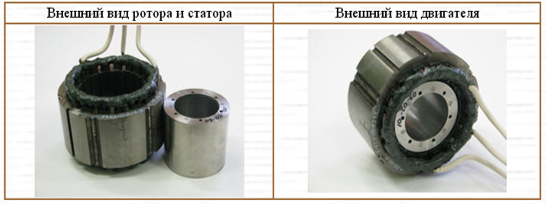
\includegraphics[width=0.8\linewidth]{image37} 
	\caption{Внешний вид 5ДБМ120- 5-2-3}
	\label{fig:5DBM120}
\end{figure}

\begin{figure}[ht]
	\centering
	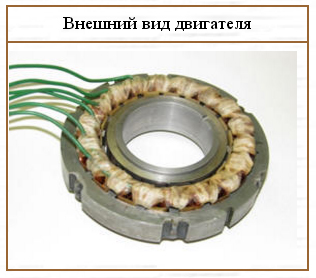
\includegraphics[]{image38} 
	\caption{Внешний вид 3ДБМ120-1-0.8-3, 5ДБМ120-2-1-3}
	\label{fig:3DBM120}
\end{figure}

\begin{figure}[ht]
	\centering
	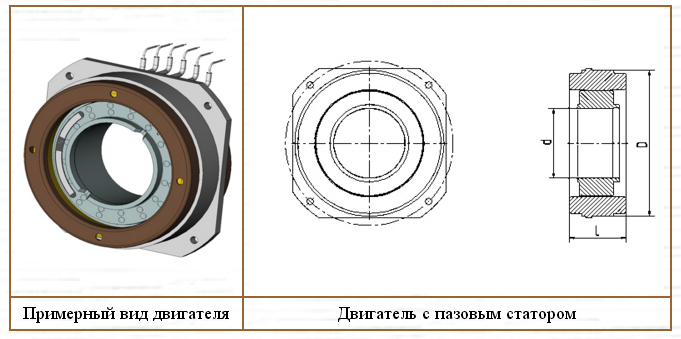
\includegraphics[width=0.8\linewidth]{image39} 
	\caption{Внешний вид 3ДБМ150-4-0.6-3, ДБМ150-4-1.5-3, 3ДБМ70-1.1-1.3-3}
	\label{fig:3DBM70}
\end{figure}

Для дальнейших исследований выбраны наиболее предпочтительные МД, удовлетворяющие требованиям ТЗ:\par

\begin{itemize}
	\item \textit{по азимуту} –  5ДБМ 120-5-2-3,
	\item \textit{по углу места} – 3 ДБМ 70-1,1-1,3-3.
\end{itemize}




\section{Уравнения движения изолированных каналов} \label{ch:ch4/sect3}

Используя линеаризованные уравнения (\ref{eq:p3:59}) полученные в разделе \ref{ch:ch3/sect10} составим зависимости положений приводов от управляющего сигнала, возмущающего воздействия и движений ЛА. В виду незначительного влияния перекрестных связей запишем уравнения (\ref{eq:p3:59}) в следующем виде:

\begin{equation}
\label{eq:p4:s3.1}
\begin{multlined}
\left( a_{11}p^{2}+b_{11}p \right)  \alpha + 
a_{11} p^2  \psi 
=
k_{1}  u_{1}- 
 M_{\textit{тр.1}},\\
\left( a_{22}p^{2}+b_{22}p \right)  \beta + c_{22}+
d_{23} p^2  \vartheta
=\\
k_{2}  u_{2} - M_{\textit{тр.2}},
\end{multlined}
\end{equation}

Перепишем уравнения относительно обобщенных координат:

\begin{equation}
\label{eq:p4:s3.2}
\begin{multlined}
\alpha= 
\frac{k_{1}}{a_{11}p^{2}+b_{11}p} u_{1} - 
\frac{1}{a_{11}p^{2}+b_{11}p} M_{\textit{тр.1}} - 
\frac{a_{11} p^2}{a_{11}p^{2}+b_{11}p}  \psi  ,\\
\beta=
\frac{k_{2}}{a_{22}p^{2}+b_{22}p} u_{2} - 
\frac{1}{a_{22}p^{2}+b_{22}p} M_{\textit{тр.2}} - \\
\frac{d_{23} p^2}{a_{22}p^{2}+b_{22}p} \vartheta -
\frac{1}{a_{22}p^{2}+b_{22}p} c_{22},
\end{multlined}
\end{equation}

Из выражения (\ref{eq:p4:s3.2}) следует, что уголы поворота ОЭП зависит не только от управления, но и от моментов трения, дисбаланса ($c_{22}=M_{\textit{дб}}$) и движений носителя. Для дальнейшего использования выражение (\ref{eq:p4:s3.2}) запишем в виде:

\begin{equation}
\label{eq:p4:s3.3}
\begin{aligned}
\alpha= 
W_{n1}(p) u_{1} - 
W_{f1}(p) M_{\textit{тр.1}} - 
W_{\psi 1}(p) \dot \psi  ,\\
\beta=
W_{n2}(p) u_{2} - 
W_{f2}(p) (M_{\textit{дб}} + M_{\textit{тр.2}}) - 
W_{\vartheta}(p) \dot \vartheta,
\end{aligned}
\end{equation}

где
ПФ азимута по управлению:
\begin{equation}
\label{eq:p4:s3.4}
\begin{multlined}
W_{n1}(p) = 
\frac{k_{1}}{a_{11}p^{2}+b_{11}p} = 
\frac{K_{n1}}{(T_{M1} T_{e1} p^2 + T_{M1} p +1)p} = 
\frac{K_{n1}}{R_1(p) p};
\end{multlined}
\end{equation}
ПФ азимута по возмущению:
\begin{equation}
\label{eq:p4:s3.5}
\begin{multlined}
W_{f1}(p) = \frac{1}{a_{11}p^{2}+b_{11}p} =  
\frac{K_{m1} (T_{e1} p +1)}{(T_{M1} T_{e1} p^2 + T_{M1} p +1)p} = 
\frac{K_{m1} R_{e1}(p)}{R_1(p)p};
\end{multlined}
\end{equation}
ПФ азимута от движения носителя:
\begin{equation}
\label{eq:p4:s3.6}
\begin{multlined}
W_{\psi}(p) = \frac{a_{11} p^2}{a_{11}p^{2}+b_{11}p} = 
\frac{T_{M1}(T_{e1} p +1)}{(T_{M1} T_{e1} p^2 + T_{M1} p +1)} = 
\frac{T_{M1}R_{e1}(p)}{R_1(p)};
\end{multlined}
\end{equation}
где 
\begin{equation}
\label{eq:p4:tt1}
\begin{aligned}
T_{M1} =\frac{R_1 (B_1 + B(\beta_0))}{C_{m1}C_{e1}},
T_{e1} = L_1/R_1,
\end{aligned}
\end{equation}

\begin{equation}
\label{eq:p4:kk1}
\begin{aligned}
K_{n1}=\frac{1}{C_{e1}},
K_{m1}= \frac{R_1}{C_{m1}C_{e1}}.
\end{aligned}
\end{equation}

ПФ угла места по управлению:
\begin{equation}
\label{eq:p4:s3.7}
\begin{multlined}
W_{n2}(p) = \frac{k_{2}}{a_{22}p^{2}+b_{22}p} = 
\frac{K_{n2}}{(T_{M2} T_{e2} p^2 + T_{M2} p +1)p} = 
\frac{K_{n2}}{R_2(p)p};
\end{multlined}
\end{equation}
ПФ угла места по возмущению:
\begin{equation}
\label{eq:p4:s3.8}
\begin{multlined}
W_{f2}(p) = \frac{1}{a_{22}p^{2}+b_{22}p} =  
\frac{K_{m2}(T_{e2} p + 1)}{(T_{M2} T_{e2} p^2 + T_{M2} p +1)p} = 
\frac{K_{m2}R_{e2}(p)}{R_2(p)p};
\end{multlined}
\end{equation}
ПФ угла места от движения носителя:
\begin{equation}
\label{eq:p4:s3.9}
\begin{multlined}
W_{\vartheta}(p) = \frac{d_{23} p^2}{a_{22}p^{2}+b_{22}p} = 
\frac{d_{23} T_{M2}(T_{e2} p + 1)}{(T_{M2} T_{e2} p^2 + T_{M2} p +1)} = 
\frac{d_{23} T_{M2}R_{e2}(p)}{R_2(p)};
\end{multlined}
\end{equation}
где 
\begin{equation}
\label{eq:p4:tt2}
\begin{aligned}
T_{M2} =\frac{R_1 C_2}{C_{m2}C_{e2}},
T_{e2} = L_2/R_2,
\end{aligned}
\end{equation}

\begin{equation}
\label{eq:p4:kk2}
\begin{aligned}
K_{n2}=\frac{2}{C_{e2}},
K_{m2}= \frac{R_2}{C_{m2}C_{e2}}.
\end{aligned}
\end{equation}

Запишем в матричной форме

\begin{equation}
\label{eq:p4:s3.3+}
\begin{aligned}
q = W_n(p) u - W_f(p) M_{\textit{н}} - W_{\textit{ла}} (p)\omega,
\end{aligned}
\end{equation}
где
\begin{equation}
\label{eq:p4:s3.4+}
\begin{aligned}
W_n(p) = K_n R(p)^{-1} \dfrac{1}{p}= \left( \begin{array}{c c}
W_{n1}(p) & 0 \\
0 & W_{n2}(p)
\end{array}\right),
u = \left( \begin{array}{c}
u_1 \\
u_2
\end{array}\right),\\
W_f(p) = K_m R_e(p) R(p)^{-1} \dfrac{1}{p}= \left( \begin{array}{c c}
W_{f1}(p) & 0 \\
0 & W_{f2}(p)
\end{array}\right),
M_{\textit{н}} = \left( \begin{array}{c}
M_{\textit{тр.1}} \\
M_{\textit{дб}} + M_{\textit{тр.2}}
\end{array}\right),\\
W_{\textit{ла}}(p) = T_m R_e(p) R(p)^{-1} = \left( \begin{array}{c c}
W_{\psi}(p) & 0 \\
0 & W_{\vartheta}(p)
\end{array}\right),
\omega = \left( \begin{array}{c}
\dot \psi \\
\dot \vartheta
\end{array}\right),           
\end{aligned}
\end{equation}
здесь
\begin{equation}
\label{eq:p4:s3.10}
\begin{aligned}
K_n = \left( \begin{array}{c c}
K_{n1} & 0 \\
0 & K_{n2}
\end{array}\right),
K_m = \left( \begin{array}{c c}
K_{m1} & 0 \\
0 & K_{m2}
\end{array}\right), 
T_M = \left( \begin{array}{c c}
T_{M1} & 0 \\
0 & T_{M2}
\end{array}\right), \\
R(p) = \left( \begin{array}{c c}
T_{M1} T_{e1} p^2 + T_{M1} p +1 & 0 \\
0 & T_{M2} T_{e2} p^2 + T_{M2} p +1
\end{array}\right), \\
R_e(p) = \left( \begin{array}{c c}
T_{e1} p + 1 & 0 \\
0 & T_{e2} p + 1
\end{array}\right).
\end{aligned}
\end{equation}

\begin{comment}
\subsection{Уравнения движения привода по азимуту} \label{subsec:ch4/sect3/sub1}

Линеаризованные уравнения движения азимутального привода совместно с объектом управления запишутся [29] [30] [31] [32] [33] [34]:

\subsection{Уравнения движения привода по углу места} \label{subsec:ch4/sect3/sub2}
\end{comment}

\section{Синтез алгоритмов} \label{ch:ch4/synthesis}

\subsection{Синтез алгоритмов и моделирование программного устройства} \label{ch:ch4/sect2+}

\subsubsection{Режим наведения} \label{subsec:ch4/sect2/sub1}

Режим наведения должен осуществляться в пределах заданых углов относительно ЛА ($\varDelta\alpha$) за время ($\varDelta t$). Для решения этой задачи управления рассмотрим оптимальное управление по быстродействию [3, 27].

Задача устройства состоит в том чтобы выдать оптимальную траекторию движения основываясь на следующих условиях:
\begin{enumerate}
	\item средняя скорость разворота должна удовлетворять требованиям ТУ: 
	$\frac{\varDelta\alpha}{\varDelta t}$
	\item скорость движения в начальный и конечным момент должна быть равна 0
	\item программный угол не должен выходить за заданые пределы
\end{enumerate}

Построим программное устройство (ПУ), предназначенное для выдачи требуемой программной траектории движения оптической оси на основе решения уравнений:
\begin{equation}
\label{eq:p4:2+.1}
\begin{alignedat}{2}
\varDelta\alpha = \dfrac{\ddot{\alpha}{\varDelta t}^2}{4}
\end{alignedat}
\end{equation}

Схема моделирования ПУ приведена на рисунке \ref{fig:model_control}. Фрагмент решения уравнений (\ref{eq:p4:2+.1}) приведен далее (рисунок \ref{fig:model_control_graph}).

\begin{figure}[ht]
	\centering
	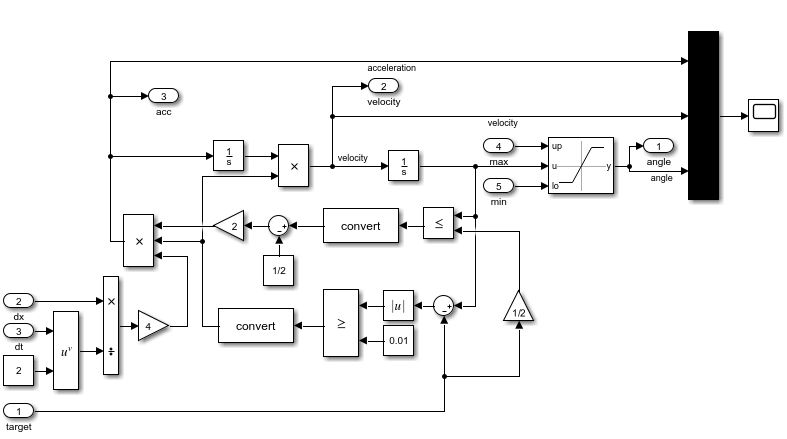
\includegraphics[width=1.0\linewidth]{model_control} 
	\caption{Схема моделирования программного устройства}
	\label{fig:model_control}
\end{figure}

Для задания необходимой программной траектории достаточно задать угол (обозначен как "target" на рисуноке \ref{fig:model_control}), на который  необходимо перевести оптическую ось ОЭП, задать скорость разворота (обозначен как "dx" и "dt" на рисуноке \ref{fig:model_control}) и задать предельные углы разворота (обозначен как "max" и "min" на рисуноке \ref{fig:model_control}). 

\begin{figure}
	\centering
	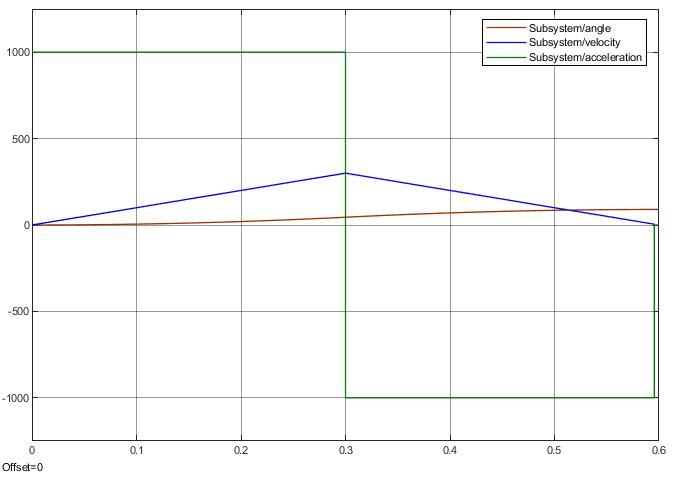
\includegraphics[width=0.7\linewidth]{model_control_graph}
	\caption{График ускорения, скорости и координаты программного движения}
	\label{fig:model_control_graph}
\end{figure}

\subsection{Синтез возмущений} \label{ch:ch4/sect2+1}

Из технических требований (таблица \ref{tab:SAU_PARAM}) известны условия при которых должна работать ОЭС. Эти воздействия можно описать в виде уравнений:
\begin{itemize}
	\item \( \omega  \left( t \right) = 12 \textit{град/с} \) ,
	\item \(  \omega _{1} ( t ) =1.38sin \left( 6.28 t \right) \),
	\item \( \omega_2 (t) = 0.21 sin(t) \).
\end{itemize}

\begin{figure}[ht]
	\centering
	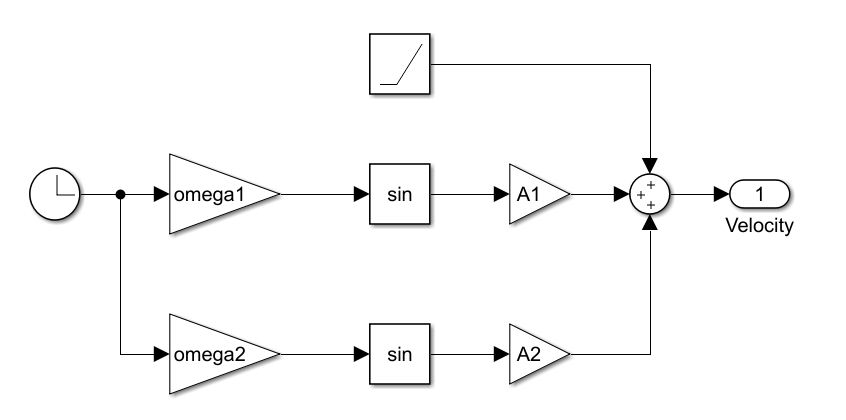
\includegraphics[width=1.0\linewidth]{1} 
	\caption{Блок модели внешних возмущений}
	\label{fig:la_model}
\end{figure}

При этом учтены следующие предельно-возможные возмущения: 
\begin{itemize}
	\item момент силы нагрузки $M_{\textit{н1}} = 2.1425 \textit{Нм}$,
	\item скорость \( \dot \psi  \left( t \right) = 12 \textit{град/с} \) ,
	\item ускорения \(  \ddot \psi _{1} \left( t \right) =1.38sin \left( 6.28 t \right) \),
	\item \( \ddot \psi_2 (t) = 0.21 sin(t) \).
\end{itemize}

\subsection{Синтез алгоритмов управления ОЭП} \label{ch:ch4/sect4-}

В соответствии с ТЗ управление ОЭП проводится в двух режимах:
наведения ОЭП на объект наблюдения (ОН) и стабилизации оптической оси относительно направления на ОН. 

Синтез алгоритмов управления проводился частотным методом \cite[]{Bessekerski} для каждого из режимов. На основе полученных законов управления разработаны компьютерные модели (КМ) линейной и нелинейной САУ в среде Simulink MatLAB и проведены исследования динамики САУ с помощью КМ в режимах наведения и стабилизации при действии возмущений, оговоренных в ТЗ.

Структурная схема САУ изолированного канала показана на рисунке \ref{fig:structured_SAU}.

\begin{figure}[ht]
	\centering
	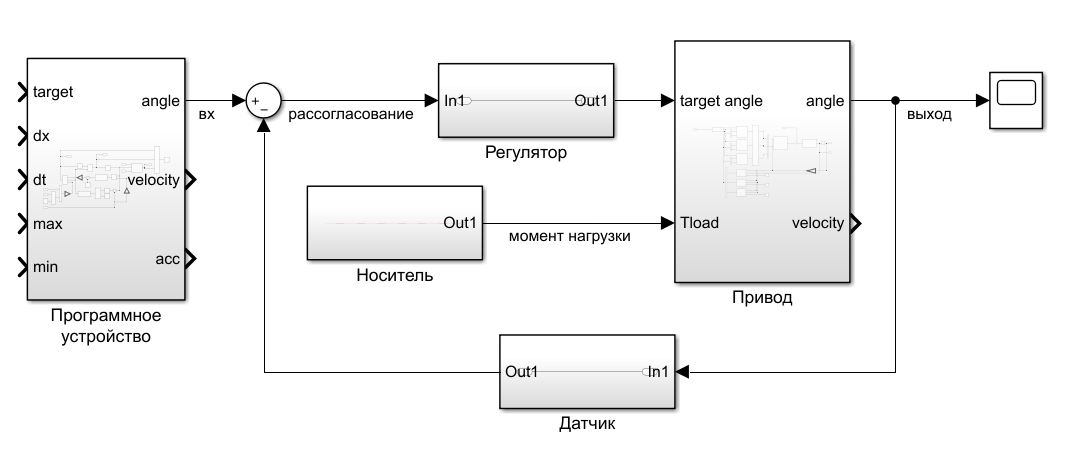
\includegraphics[width=0.8\linewidth]{structured_SAU}
	\caption{Структурная схема САУ}
	\label{fig:structured_SAU}
\end{figure}

Программное устройство определяет режим работы и задает целевое значение положения ротора канала, регулятор обеспечивает оптимальную работу привода, привод - объект управления , 
датчик угла измеряет положение ротора, "носитель" определяет внешние возмущающие факторы влияющие на систему.

%\subsection{Азимут} \label{ch:ch4/sect4-/sub1}

В соответствии с уравнением (\ref{eq:p4:s3.3+}) и параметрами (таблица \ref{tab:DBM}) приводов выбраных ранее в разделе \ref{ch:ch4/sect2} МД 5ДБМ 120-5-2-3 (новая разработка) для азимута и МД ДБМ 70-1,1-1,3-3 для угла места оценим параметры приводов необходимые для дальнейших расчетов при исходных данных для:
\begin{itemize}
	\item \textit{канала азимута (1)}
	
	\[  R_1 = 0.32 \textit{Ом}, 
	T_{e1} = 0.1 \textit{мс}, 
	J_{p1} = 0.75 \cdot 10^{-5} \textit{кг м}^2,  
	u_\textit{н1} = 27 \textit{В},
	i_\textit{н1} = 75 \textit{А} \]
	
	\begin{equation}
	\label{eq:p4:sec4/2}
	\begin{multlined}
	C_{e1}=
	\frac{u_\textit{н1}-i_{\textit{н1}}R_{1}}{ \omega _{\textit{н}}}=
	\frac{27-75 \cdot 0.32}{11.1}=
	0.27 \textit{Вс/рад},
	\end{multlined}
	\end{equation}
	
	\begin{equation}
	\label{eq:p4:sec4/3}
	\begin{multlined}
	C_{m1}=
	\frac{M_{\textit{н}}}{i_{\textit{н}}}=
	\frac{27.11}{75}=0.36 \textit{Нм/А},
	\end{multlined}
	\end{equation}
	
	\item \textit{канала угла места (2)}
	
	\[  R_2 = 0.485 \textit{Ом}, 
	T_{e2} = 0.4 \textit{мс}, 
	J_{p2} = 0.2510 \cdot 10^{-5} \textit{кг м}^2,  
	u_\textit{н2} = 27 \textit{В},\]
	
	\[C_{e2} = 0.12 \textit{Вс/рад}, 
	C_{m2} = 0.12 \textit{Нм/А},
	\]
	
	\item \textit{внешних возмущениях} (таблица \ref{tab:SAU_PARAM})
	
	\begin{equation}
	\label{eq:p4:sec4/1}
	\begin{multlined}
	\omega _{\textit{н}}=
	\alpha _{\textit{пр}} + A_{1} \omega _{1} + A_{2} \omega _{2} + \alpha _{0} =\\
	10.47 + 0.21 \cdot 1 + 0.035 \cdot 6.28 + 0.21 = 11.1 \textit{рад/с},
	\end{multlined}
	\end{equation}

\end{itemize}
где  \(  \omega _{\textit{н}}- \) максимальное значение номинальной угловой скорости прибора, А\textsubscript{1} , А\textsubscript{2 }- амплитуды колебаний на частотах 0.16 Гц и 1Гц,  \( \dot \alpha _{0} \)  - угловая скорость носителя,  \( \dot \alpha _{\textit{пр}} \) - программный поворот прибора.

\begin{itemize}
	\item \textit{канала азимута (1)}
	\begin{equation}
	\label{eq:p4:sec4/4}
	\begin{alignedat}{2}
	T_{M1}=
	\frac{ \left( J_{\textit{н1}}+J_{01} \right) R_{1}}{C_{m1}C_{e1}}=\frac{ \left( 0.327 + 0.75 \cdot 10^{-5} \right) 0.32}{0.36 \cdot 0.27}=
	1.08 \textit{c} ,\\
	K_{n1} = \frac{1}{C_{e1}} = \frac{1}{0.27} = 3.7 \textit{рад/Вс},\\
	K_{m1} = \frac{R_1}{C_{e1} C_{m1}} = \frac{0.32}{0.27 \cdot 0.36} = 3.29 \textit{рад/Нмс},
	\end{alignedat}
	\end{equation}
	
	\item \textit{канала угла места (2)}
	\begin{equation}
	\label{eq:p4:sec4/4+}
	\begin{alignedat}{2}
	T_{M2}=
	\frac{ \left( J_{\textit{н2}}+J_{02} \right) R_{2}}{C_{m2}C_{e2}}=\frac{ \left( 0.2510 \cdot 10^{-5} + 8.4 \cdot 10^{-3} \right) 0.485}{0.12 \cdot 0.12}=
	0.2913 \textit{c} ,\\
	K_{n2} = \frac{1}{C_{e2}} = \frac{1}{0.12} = 8.33 \textit{рад/Вс},\\
	K_{m2} = \frac{R_2}{C_{e2} C_{m2}} = \frac{0.485}{0.12 \cdot 0.12} = 33.68 \textit{рад/Нмс},
	\end{alignedat}
	\end{equation}
	
\end{itemize}



Для оценки требуемой добротности САУ по скорости запишем передаточную функцию по ошибке в соответствии с уравнениями:\par


\begin{equation}%\tag{414}
\label{eq:p4:414}
\begin{alignedat}{2}
\begin{comment}
\left. \begin{array}{ll}
\alpha =W_{n1} \left( p \right) U_{1}-W_{f1} \left( p \right) M_{H1}-W_{ \psi } \left( p \right) \dot \psi\\
\Delta  \alpha = \alpha _{\textit{пр}}- \alpha\\
U_{1}=K_{\textit{д1}}\cdot K_{y1} \cdot W_{k1} \left( p \right)  \Delta  \alpha \\
\end{array}  \right\rbrace \\ 
\end{comment}
\left. \begin{array}{ll}
q = W_n(p) u - W_f(p) M_{\textit{н}} - W_{\textit{ла}} (p)\omega\\
\Delta  q = q_{\textit{пр}}- q\\
u = K_{\textit{д}}\cdot K_{y} \cdot W_{k} \left( p \right)  \Delta  q \\
\end{array}  \right\rbrace  
\end{alignedat}
\end{equation}
где
$ \Delta  q = \left( \begin{array}{l}
\Delta \alpha\\
\Delta \beta
\end{array} \right)  $ - рассогласование,

$ q_{\textit{пр}} = \left( \begin{array}{l}
\alpha_{\textit{пр}}\\
\beta_{\textit{пр}}
\end{array} \right)  $ - программное управление,

$K_{\textit{д}} = \left( \begin{array}{cc}
K_{\textit{д1}} &0\\
0&K_{\textit{д2}}
\end{array} \right)  $ - коэффициенты усиления датчиков,

$K_{\textit{y}} = \left( \begin{array}{cc}
 K_{y1}  &0\\
0& K_{y2} 
\end{array} \right)  $ - коэффициенты усиления преобразователей,

$W_{k} \left( p \right) = \left( \begin{array}{cc}
 W_{k1} \left( p \right) &0\\
0& W_{k2} \left( p \right)
\end{array} \right)  $ - передаточные функции регуляторов.
Из уравнений (\ref{eq:p4:414}) получим:

\begin{comment}
\begin{equation}%\tag{415}
\label{eq:p4:415}
\begin{alignedat}{2}
\Delta  \alpha =\frac{1}{1+W_{1} \left( p \right) } \alpha _{\textit{пр}}-\frac{W_{f1} \left( p \right) }{1+W_{1} \left( p \right) }M_{H1}-\frac{W_{ \psi } \left( p \right) }{1+W_{1} \left( p \right) } \dot \psi,
\end{alignedat}
\end{equation}
\end{comment}

\begin{equation}%\tag{415}
\label{eq:p4:415}
\begin{alignedat}{2}
\Delta  q = 
(W(p)+E_2)^{-1} q _{\textit{пр}}-
(W(p)+E_2)^{-1} W_{f1} \left( p \right) M_{H}-\\
(W(p)+E_2)^{-1} W_{\textit{ла}} (p) \omega,
\end{alignedat}
\end{equation}

где 
\begin{comment}
\begin{equation}
\label{eq:p4:415+}
\begin{alignedat}{2}
 W_{1} \left( p \right) =
 K_{\textit{д1}}K_{\textit{у1}}W_{k1} \left( p \right) W_{n1} \left( p \right) =
 W_{k1} \left( p \right) \frac{K_{c1}}{ \left( T_{M1}T_{e1}p^{2}+T_{M1}p+1 \right) p}; \\
  K_{c1}=K_{\textit{д1}}K_{\textit{у1}}K_{k1}K_{n1}.
\end{alignedat}
\end{equation}
\end{comment}
\begin{equation}
\label{eq:p4:415+}
\begin{alignedat}{2}
W \left( p \right) =
K_{\textit{д}}K_{\textit{у}}W_{k} \left( p \right) W_{n} \left( p \right) =
W_{k} \left( p \right) K_{c} R(p)^{-1}  \dfrac{1}{p}; \\
K_{c}=K_{\textit{д}}K_{\textit{у}}K_{k}K_{n}.
\end{alignedat}
\end{equation}

В установившемся режиме ($t\rightarrow0, p\rightarrow0$) имеем\par
\begin{comment}
\begin{equation}
\label{eq:p4:415+2}
\begin{alignedat}{2}
\Delta  \alpha =
\frac{1}{K_{c1}} \dot \alpha_{\textit{пр}} + \frac{K_{m1}}{K_{c1}}M_{H1} - \frac{T_{M1}}{K_{c1}} \dot \psi ,
M_{Н1}=M_{\textit{ТР1}}+M_{\textit{дб1}}=2.1425\textit{Нм}
\end{alignedat}
\end{equation}
\end{comment}
\begin{equation}
\label{eq:p4:415+2}
\begin{alignedat}{2}
\Delta  q =
K_{c}^{-1} \dot q_{\textit{пр}} + K_{m} K_{c}^{-1} M_{\textit{н}} - T_{m} K_{c}^{-1} \omega ,\\
M_{\textit{н}} = \left( \begin{array}{c}
M_{\textit{тр.1}} \\
M_{\textit{дб}} + M_{\textit{тр.2}}
\end{array}\right)=
\left( \begin{array}{c}
2.1425\textit{Нм} \\
0.25 \textit{Нм}
\end{array}\right)
\end{alignedat}
\end{equation}

Из решения уравнения (\ref{eq:p4:2+.1}) следует, что в конечной координате наведения (при \textit{t} = 0.6c)  \( \dot q _{\textit{пр}}=0 \) , тогда коэффициент усиления разомкнутой системы можно определить по формуле \par
\begin{comment}
\begin{equation}
\label{eq:p4:416}
\begin{alignedat}{2}
K_{c1} \geq \frac{K_{m1}M_{H1}+T_{M1} \ddot \psi ^{max}}{ \Delta  \alpha ^{\textit{доп}}}
\end{alignedat}
\end{equation}
\end{comment}

\begin{equation}
\label{eq:p4:416}
\begin{alignedat}{2}
K_{c} \geq E_2 {(K_{m}M_{\textit{н}}+T_{m} \dot \omega ^{max})}{ \Delta  {q ^{\textit{доп}}}^{-1}}
\end{alignedat}
\end{equation}

Оценим  \( K_{c}, \dot \omega ^{max} \), где 

$A_1 = 12 \textit{град} = 0.21 \textit{рад}, \omega_1 = 1 \frac{1}{c}$

$A_2 = 2 \textit{град} = 0.035 \textit{рад}, \omega_2 = 6.28 \frac{1}{c}$

$\varDelta q^{\textit{доп}} =  0.5 \textit{град} = 0.0087 \textit{рад}$
\[ 
K_{c}=
\left( \begin{array}{cc}
\frac{3.29 \cdot 2.14 + 1.08 \cdot 1.6}{0.0087} \frac{1}{c}&0 \\
0& \frac{33.68 \cdot 0.25 + 0.2913 \cdot 1.6}{0.0087}
\end{array}\right)\frac{1}{c}=
\left( \begin{array}{cc}
940.85 &0 \\
0& 1021.38
\end{array}\right) \frac{1}{c} \rightarrow
\]

\[
\left( \begin{array}{cc}
1200 &0 \\
0& 1250
\end{array}\right)\frac{1}{c}
. 
\] \par

Оценим устойчивость системы (\ref{eq:p4:414}), используя частотный критерий Найквиста \cite[]{Bessekerski}. Для этого, используя полученные параметры системы, построим частотные характеристики (ЧХ): (ЛAX –логарифмическая амплитудная характеристика, ЛФХ – логарифмическая фазовая характеристика) разомкнутой системы $W_1(j \omega)$ (рисунки \ref{fig:LogAmpChar1},\ref{fig:LogAmpChar2}).\par


\begin{figure}[ht]
	\centering
	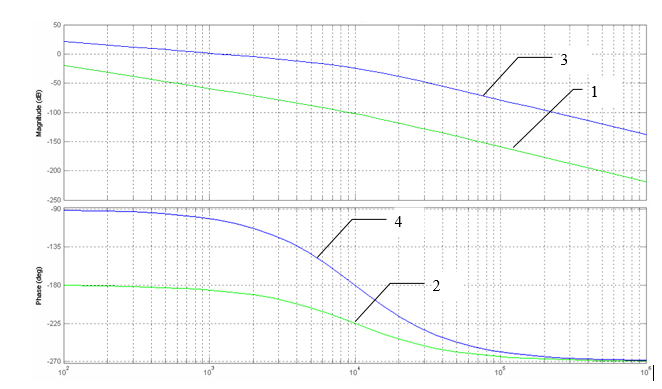
\includegraphics[width=1.0\linewidth]{image51} 
	\caption{LAX и LФХ разомкнутой системы. 1-ЛАХ, 2-ЛФХ ЧХ1($W_{k1}(p)=1 $), 3-ЛАХ, 4-ЛФХ ЧХ2 ($T_{k11} = 1.08 c$, $T_{k21} = 0.0001 c$}
	\label{fig:LogAmpChar1}
\end{figure}

\begin{figure}[ht]
	\centering
	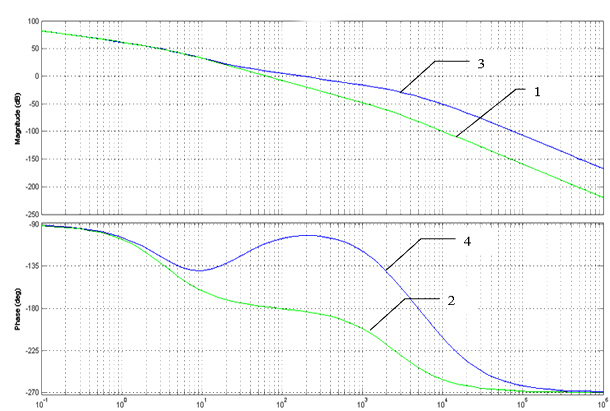
\includegraphics[width=1.0\linewidth]{image66} 
	\caption{LAX и LФХ разомкнутой системы. 1-ЛАХ, 2-ЛФХ ЧХ1($W_{k1}(p)=1 $), 3-ЛАХ, 4-ЛФХ ЧХ2 ($T_{k12} = 0.04 c$, $T_{k22} = 0.001 c$}
	\label{fig:LogAmpChar2}
\end{figure}

Из анализа ЧХ1 (рисунки \ref{fig:LogAmpChar1},\ref{fig:LogAmpChar2}, ЧХ-1) видно, что исходная САУ (\ref{eq:p4:414}) без коррекции (${W_k}_i=1$) находится на границе устойчивости. Для устойчивости рассматриваемой системы с требуемыми запасами (по фазе  $ \geq $  (45-60) град., L~$\geq$ (6-15) дб),\ необходимые для обеспечения приемлемых переходных процессов САУ, введем корректирующее последовательное фазоопережающее устройство с ПФ:

\begin{equation}%\tag{417}
\label{eq:p4:417}
\begin{alignedat}{2}
{W_{k}}_{ii} \left( p \right) =K_{ki}\frac{ \left( T_{k1i}p+1 \right) }{ \left( T_{k2i}p+1 \right) }.
\end{alignedat}
\end{equation}

Выбором параметров (\ref{eq:p4:417}) можно обеспечить устойчивость и требуемые запaсы устойчивости и качество переходного процесса. 
\begin{itemize}
	\item \textit{Для азиимута}\par
	$T_{k11} = 1.08 c$, $T_{k2} = (0.0001  \div 0.001) c$  САУ устойчива (рисунок \ref{fig:LogAmpChar1} ЧХ-2), имея запасы устойчивости по амплитуде $\varDelta L = (24 \div 19)$ дБ и фазе $\varDelta \varphi = (86 \div 53)$ град,
	\item \textit{Для угла места}\par
	$T_{k12} = 0.04 c$, $T_{k22} =  0.001 c$  САУ устойчива (рисунок \ref{fig:LogAmpChar2} ЧХ-2), имея запасы устойчивости по амплитуде $\varDelta L = 30$ дБ и фазе $\varDelta \varphi = 72$ град.
\end{itemize}

На основе полученных параметров синтезированного регулятора, модели ПУ (Рисунок \ref{fig:model_control}) и структурой схемы (рисунок \ref{fig:structured_SAU}) разработана компьютерная имитационная модель (КИМ) линейной САУ (рисунок \ref{fig:az}) в соответствии с уравнениями (\ref{eq:p4:414}) , используя MatLAB Simulink. Содержание блока «Программное движение» показано на рисунке \ref{fig:model_control}, «Возмущения». 

\begin{figure}[ht]
	\centering
	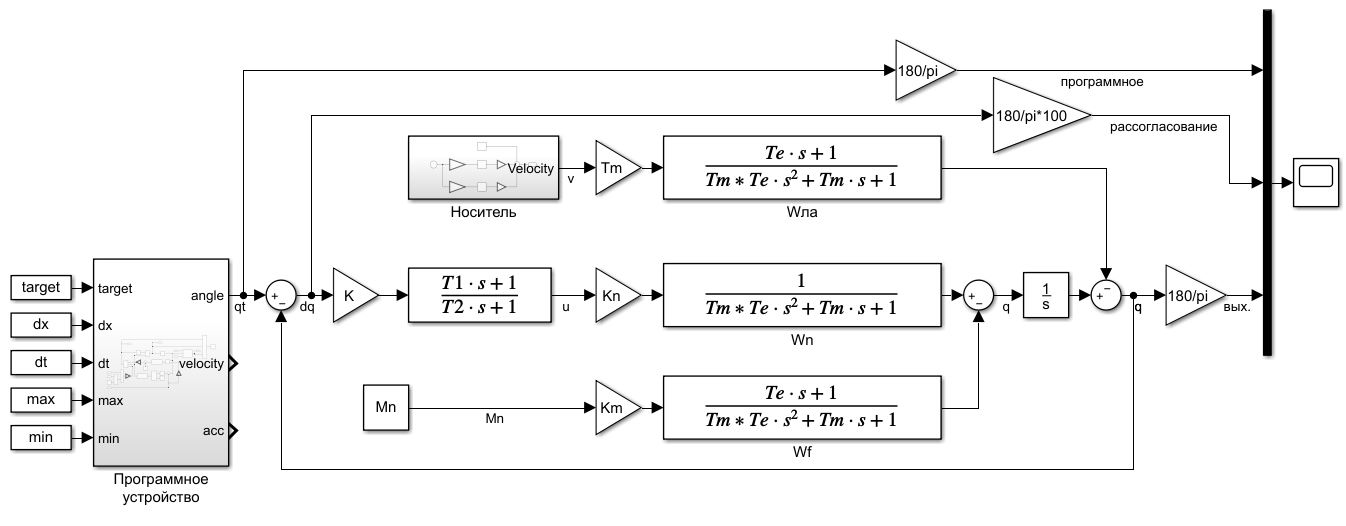
\includegraphics[width=1.0\linewidth]{az} 
	\caption{КИМ1,2 линейной САУ в режиме наведения}
	\label{fig:az}
\end{figure}

Исходные данные для моделирования азимутального канала указаны в листинге \ref{lst:az}, для канала угла места в листинге \ref{lst:um}. 

\begingroup
\captiondelim{ } % разделитель идентификатора с номером от наименования
\lstinputlisting[caption={Исходные данные для КИМ1 (канал азимута)},label={lst:az}]{listings/az_3.m}
\endgroup

\begingroup
\captiondelim{ } % разделитель идентификатора с номером от наименования
\lstinputlisting[caption={Исходные данные для КИМ2 (канал угла места)},label={lst:um}]{listings/um_3.m}
\endgroup

Разработанная КИМ1,2 САУ для режима наведения (рисунок \ref{fig:az}) позволяет проводить исследования динамики процесса управления ОЭП, варьируя параметрами регулятора, объекта управления и возмущающими воздействиями в широких пределах при различных заданных углах наведения в диапазоне  \( \alpha = \pm 180 \textit{град}\), \( \beta = (+30 \div -60) \textit{град}\).

На рисунке ниже (рисунках \ref{fig:az_},\ref{fig:um_}) приведены переходные и установившиеся процессы наведения ОЭП на угол равный \( \alpha = 180  \textit{град}, \beta = -60  \textit{град} \) при действии указанных выше возмущений ($M_{\textit{н}}, \omega(t)$). Из анализа процессов наведения (рисунки~\ref{fig:az_}, \ref{fig:um_}) при максимальном угле наведения (\( \alpha = 180  \textit{град}, \beta = -60  \textit{град} \)) погрешность наведения не превышает $\Delta \alpha = 0.5 \textit{град}, \Delta \beta = 0.5 \textit{град}$, при этом коэффициенты датчика и усилителя должны быть не менее $K_{\textit{д1}} K_{\textit{у1}} K_{\textit{к1}} = 320 \textit{В/рад}, K_{\textit{д2}} K_{\textit{у2}} K_{\textit{к2}} = 150 \textit{В/рад}$.

\begin{figure}[ht]
	\centering
	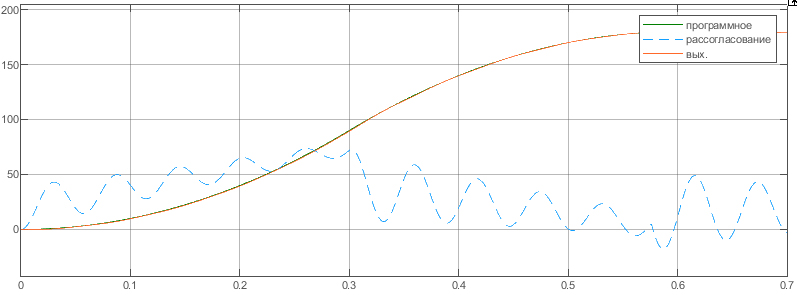
\includegraphics[width=1.0\linewidth]{az_} 
	\caption{Процессы наведения ОЭП по каналу азимута}
	\label{fig:az_}
\end{figure}

\begin{figure}[ht]
	\centering
	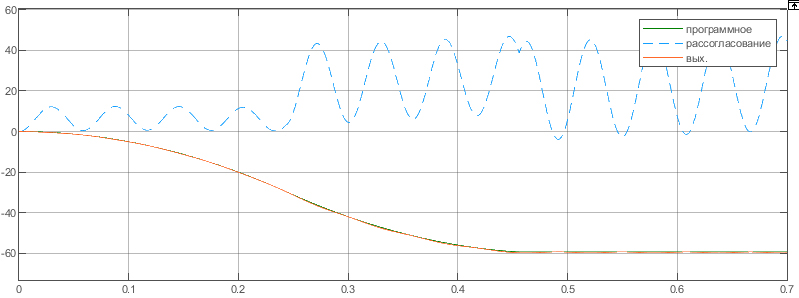
\includegraphics[width=1.0\linewidth]{um_} 
	\caption{Процессы наведения ОЭП по каналу угла места}
	\label{fig:um_}
\end{figure}

\subsection{Синтез нелинейной САУ} \label{subsec:ch4/sect4/sub2}

Основными нелинейностями, влияющие на динамику САУ, являются:
\begin{itemize}
	\item насыщение в усилителе мощности (\textit{U\textsubscript{max} =  27В});
	\item дискретность преобразователя сигналов  СКВТ в качестве датчика угла (ДУ), для 14 разрядов дискрета составляет ($\varDelta_{\textit{ду}} = 1.3183 \textit{угл. мин} = 3.83 \cdot 10^{-4} \textit{рад}$), принципиальная схема датчика показана на рисуноке \ref{fig:SKVT2}, в соответствии с \cite[]{1310HM025} для 14 разрядного преобразования датчик можно представить в виде дискретного звена со следующей ПФ:
	\begin{equation}
	\label{eq:p4:SKVT}
	\begin{alignedat}{2}
	G ( z ) =\frac{ 1 - a z^{-1} }{ 1 - b z^{-1} } = \frac{ 1 - 8191/8192 z^{-1} }{ 1 - 8182/8192 z^{-1} },
	\end{alignedat}
	\end{equation}
	имеет ЧХ разомкнутого контура показанную на рисунке \ref{fig:SKVT3};
	\item частота широтно-импульсной модуляции (ШИМ), описывается следующей передаточной функцией:
	\begin{equation}
	\label{eq:p4:PWM}
	\begin{alignedat}{2}
	W ( p ) =k_{pwm} \frac{ e^{-p \tau_0 } }{ T_{pwm} p + 1 } = k_{pwm} \frac{ e^{-p \tau_0 } }{ T_{pwm} p + 1 },
	\end{alignedat}
	\end{equation}
	при частоте счетчика $f_y~=~16000$Гц
\end{itemize} 

\begin{figure}[ht]
	\centering
	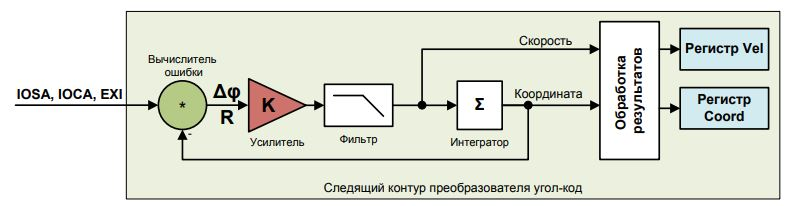
\includegraphics[width=0.8\linewidth]{SKVT2} 
	\caption{принципиальная схема цифровой части датчика СКВТ \cite[]{1310HM025}}
	\label{fig:SKVT2}
\end{figure}

Для обработки сигналов СКВТ используется микросхема преобразователя сигналов датчиков перемещения
1310НМ025 со следующими характеристиками:
\begin{itemize}
	\item Напряжение цифрового и аналоговогопитания 3,0 – 5,5 В;
	\item Разрядность преобразователякоординаты настраиваетсяпользователем от 8 до 16 бит;
	\item Частота возбуждения датчиков от 0 до 20 кГц;
	\item Генератор опорного сигнала счастотой от 20 Гц до 20 кГц;
	\item Возможно одновременноеподключение двух датчиков СКВТ или ЛРДТ;

\end{itemize}

\begin{figure}[ht]
	\centering
	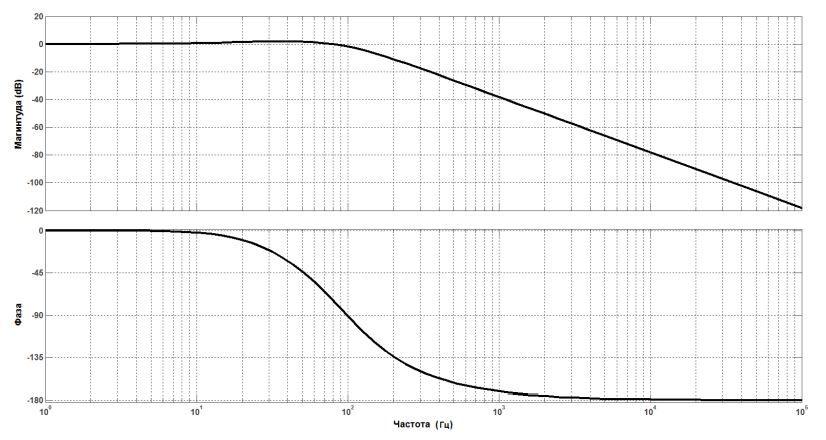
\includegraphics[width=1.0\linewidth]{SKVT3} 
	\caption{Вид типичной АЧХ и ФЧХ контура (LBW=14) \cite[]{1310HM025}}
	\label{fig:SKVT3}
\end{figure}

САУ по углу места, как и САУ по азимуту, является нелинейной и импульсной. В связи с этим будем решать те же вопросы, связанные с изучением влияния нелинейностей и дискретного характера сигналов на динамические свойства САУ. \par

\subsection{Синтез цифровой САУ } \label{subsec:ch4/sect4/sub3}

(ЦСАУ) наиболее просто проводить в частотной области методами, разработанными для непрерывных систем \cite{Bessekerski},\cite{Karpov29}. Синтез параметров будем проводить на основе  критерия  устойчивости Найквиста и частотных критериев качества регулирования   ($M_i < 1.25$, запасы устойчивости: по фазе $\varDelta \varphi_i \geq 45 $ град. и по амплитуде $\varDelta L_i \geq 6$ дБ).\par

В связи с этим отметим некоторые условия, которые необходимо выполнить и которые ограничивают область синтезируемых параметров регулятора линейной системы.\par

При исследовании устойчивости и качества регулирования САУ совместно с цифровыми вычислительными устройствами (ЦВУ) в контуре управления необходимо построить желаемую логарифмическую частотную характеристику (ЛАХ) с учетом следующих условий \cite{Bessekerski},\cite{Karpov29}.\par

\begin{enumerate}
	\item Для обеспечения требований по устойчивости и запасу устойчивости в соответствии с критерием Найквиста необходимо дополнительно выполнить неравенство:\par
	\begin{equation}%\tag{418}
	\label{eq:p4:418}
	\omega_{\textit{ср}}< \omega _{\textit{гр}}=\frac{2}{T}
	\end{equation}
	где  \(  \omega _{\textit{ср}}\) - частота среза непрерывной системы,  \(  \omega _{\textit{гр}}\) - граничная частота,  \( T- \) период повторения (квантование по времени) ЦВУ;	
	\item Малые постоянные времени ($T_i <  \omega_{\textit{ср}}^{-1}$) должны удовлетворять условию: $T_i < 0.5 T$;
	\item Переход оси нуля децибел асимптотической ЛАХ непрерывной части, разомкнутой САУ проходит при отрицательном наклоне 20 \textit{дб/дек};
	\item При построении ЛАХ разомкнутой САУ с ЦВУ в высокочастотной области  (\( \omega > \omega_{\textit{ср}} \)) следует учитывать сумму малых постоянных времени ( \(  \sum T_{i} \) ), при этом необходимо выполнить  ещё одно дополнительное условие\par	
	\begin{equation}%\tag{419}
	\label{eq:p4:419}
	\frac{T}{2}+ \sum T_{i} \leq \frac{1}{ \omega _{\textit{ср}}}\frac{M}{ \left( M+1 \right)},
	\end{equation}
	которое позволяет применять частотные методы расчета линейных систем для исследования САУ с ЦВУ в высокочастотной области.\par
\end{enumerate}

Таким образом, при выполнении условий  ЛАХ разомкнутой САУ с ЦВУ в контуре управления в низкочастотной области  (\(  \omega< \omega _{\textit{ср}} \))  можно заменить ЛАХ линейной разомкнутой САУ в этой же области. Так как в обоих каналах управления используются усилитель и датик одной конструкции, то расчеты периода квантования аналогичны для обоих каналов.


Оценим периоды квантования: 
\begin{itemize}
	\item Для ШИМ усилителя $T_{pwm} = 1/16000 = 0.0000625 c$;
	\item Для ДУ период квантования оценим из условия обеспечения измерения угла отработки (подробнее в разделе \ref{subsec:ch4/sect4/sub2}) двигателем минимальной угловой скорости
	\begin{equation}
	\alpha_0 = 12 \textit{град/сек}, T_{\textit{ду}} = \frac{\varDelta_{\textit{ду}}}{\dot \alpha_0}=
	\frac{0.0219}{12}=0.00183 c;
	\end{equation}	
\end{itemize}

Из расчетов следует, что предельным периодом квантования ЦСАУ будет $T = 0.00183 c$. С учетом условий (\ref{eq:p4:418}),(\ref{eq:p4:419}) при $M=1.1$ оценим:\par

\begin{equation}
\label{eq:p4:x}
\begin{multlined}
\omega_{\textit{гр}}=\frac{2}{T}=\frac{2}{0.00183}=1092.9 c^{-1},\\ 
\sum T_{i}=T_{\textit{e1}}+T_{k2}=0.0001+0.00005=0.00015 c, \\
\omega _{\textit{ср}} \leq 491.84 c^{-1} \rightarrow 250 c^{-1} \rightarrow log(250) = 2.398
\end{multlined}
\end{equation}

С учетом условий (\ref{eq:p4:418}),(\ref{eq:p4:419}) получены требования к линейной части ЦСАУ.\par

На основе проведенных расчетов синтезируем частотным методом \cite{Bessekerski} корректирующее звено (\ref{eq:p4:417}) с новыми параметрами: \par

\begin{equation}
\label{eq:p4:xx}
T_{k11} = 0.05 c, T_{k21} = 0.00005 c, T_{k12} = 0.05 c, T_{k22} = 0.00005 c, 
\end{equation}\par

обеспечивающие  устойчивость ЦСАУ с запасами устойчивости
\begin{itemize}
	\item \textit{для канала азимута}
	
	по амплитуде ($\varDelta L = 50$ дБ) и фазе  ($\varDelta \varphi = 83$ град) рисунок \ref{fig:DSAU},
	\item \textit{для канала угла места}
	
	по амплитуде ($\varDelta L = 28$ дБ) и фазе ($\varDelta \varphi = 82$ град)  рисунок \ref{fig:DSAU2}.
\end{itemize}

Для обеспечения требуемой точности наведения добротность САУ по скорости определена в пределах 
\begin{itemize}
	\item \textit{для канала азимута}
	
	К\textsubscript{с1}= (3590 – 3700) с\textsuperscript{-1}, соответственно - К\textsubscript{д1}К\textsubscript{к1 }К\textsubscript{у1}= (700-1000) В/рад,
	\item \textit{для канала угла места}
	
	К\textsubscript{с2}= 1250с\textsuperscript{-1}, соответственно - К\textsubscript{д2}К\textsubscript{у2} К\textsubscript{к2}= 150 В/рад.
\end{itemize}

\begin{figure}[!ht]
	\centering
	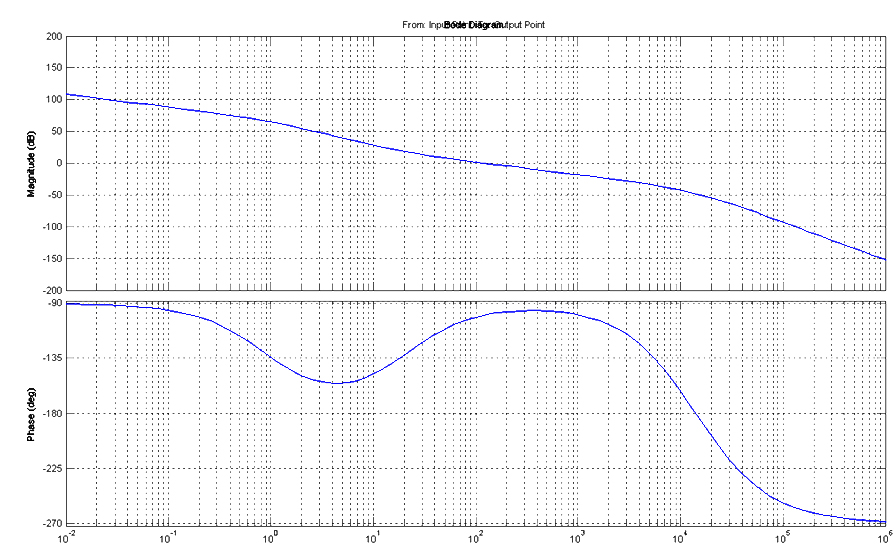
\includegraphics[width=1.0\linewidth]{image55} 
	\caption{ЛАХ и ЛФХ разомкнутой линейной части ЦСАУ канала азимута}
	\label{fig:DSAU}
\end{figure}

\begin{figure}[!ht]
	\centering
	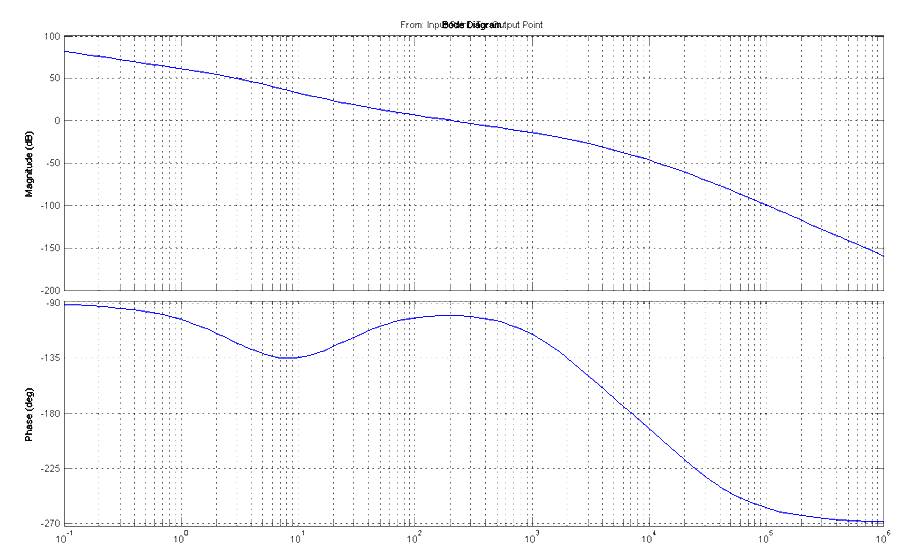
\includegraphics[width=1.0\linewidth]{image69} 
	\caption{ЛАХ и ЛФХ разомкнутой линейной части ЦСАУ канала угла места}
	\label{fig:DSAU2}
\end{figure}

\section{Моделирование и исследование динамики} \label{subsec:ch4/modeling}

\subsection{Моделирование и исследование динамики ЦСАУ} \label{subsec:ch4/sect4/sub4}

На основе синтезированных регуляторов САУ и с учетом указанных нелинейностей разработаны КИМ ЦСАУ (рисунок \ref{fig:digital_az}). Модели с учетом нелинейностей КИМ позволяют изменять величины дискретности датчика, частоту ШИМ усилителя и насыщения в УМ и проводить исследования динамики нелинейной САУ при заданных пределах этих параметров. 


\begin{figure}
	\centering
	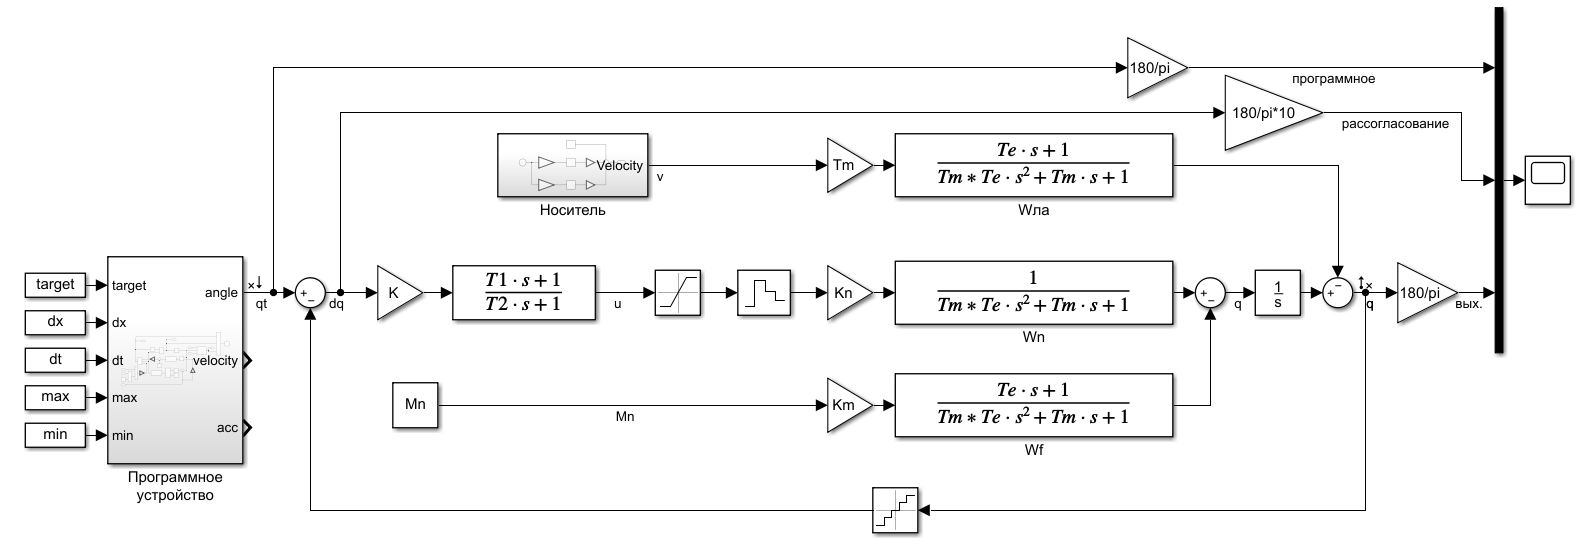
\includegraphics[width=1.0\linewidth]{digital_az} 
	\caption{КИМ 3,4 нелинейной ЦСАУ в режиме наведения}
	\label{fig:digital_az}
\end{figure}

Исходные данные для моделирования азимутального канала указаны в листинге \ref{lst:digital_az}, для канала угла места в листинге \ref{lst:digital_um}. 

\begingroup
\captiondelim{ } % разделитель идентификатора с номером от наименования
\lstinputlisting[caption={Исходные данные для КИМ3 (канал азимута)},label={lst:digital_az}]{listings/az_d.m}
\endgroup

\begingroup
\captiondelim{ } % разделитель идентификатора с номером от наименования
\lstinputlisting[caption={Исходные данные для КИМ4 (канал угла места)},label={lst:digital_um}]{listings/um_d.m}
\endgroup

На рисунках \ref{fig:az_digital} – \ref{fig:az_digital6} приведены результаты моделирования динамики наведения ОЭП с учетом указанных нелинейностей в канале азимута на угол  $\alpha=180^0$, а на рисунках \ref{fig:um_digital} – \ref{fig:um_digital5} в канале угла места на угол  $\beta=60^0$. Из анализа процессов наведения следует, что:\par

\textbf{Азимут}

- при совместном учете насыщения УМ, дискретности ДУ и ШИМ УМ, погрешность наведения на угол $180^0$  составляет $ \varDelta\alpha < 0.5^0$ (рисунок \ref{fig:az_digital}).\par

\begin{figure}
	\centering
	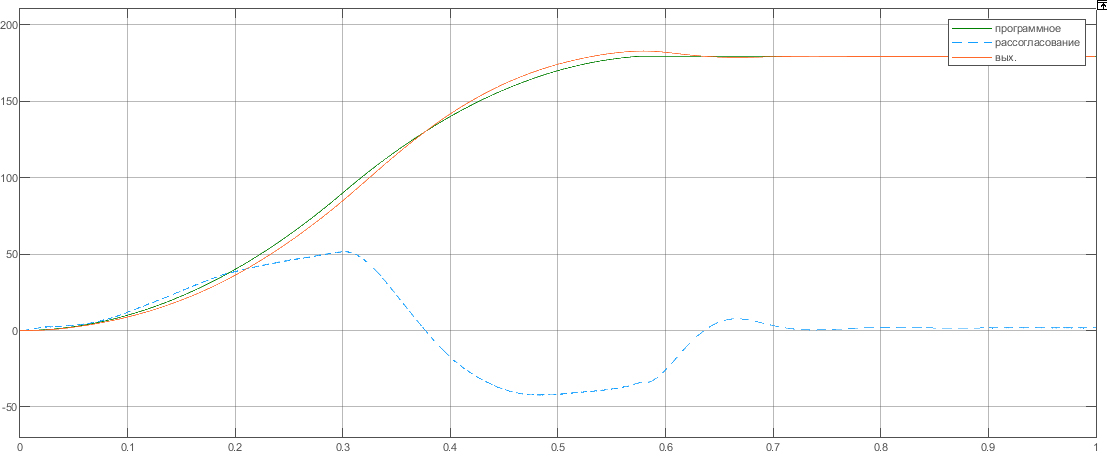
\includegraphics[width=1.0\linewidth]{az_digital1} 
	\caption{КИМ 3, Процессы наведения ОЭП с учетом насыщения УМ, дискретности ДУ и ШИМ УМ ($K_{\textit{д1}} K_{\textit{у1}} K_{\textit{к1}} = 700 \textit{В/рад}$)}
	\label{fig:az_digital}
\end{figure}

- изменение напряжения на выходе УМ в процессе наведения приведены на рисунке ниже (рисунок \ref{fig:az_digital2}). Период переключений напряжений: ($0.12   \div   1.25$) мс.\par

\begin{figure}
	\centering
	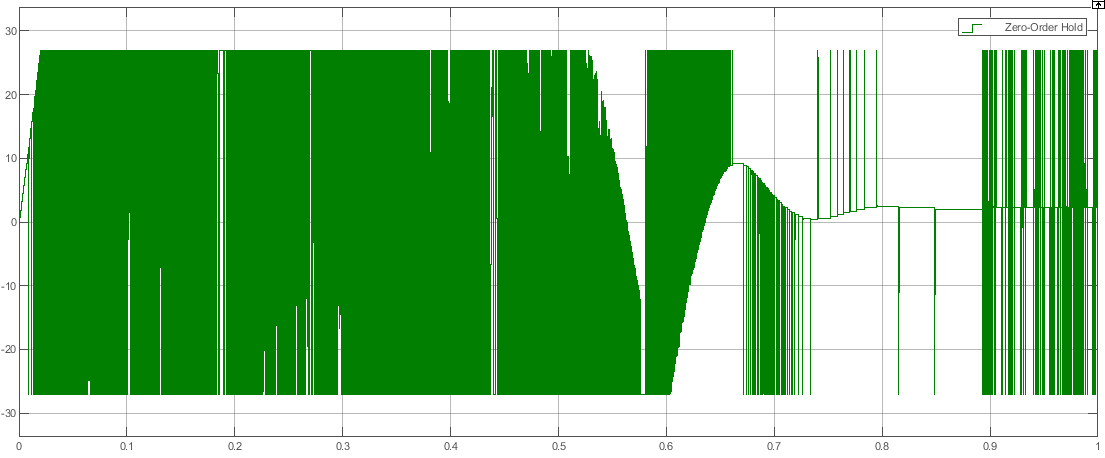
\includegraphics[width=1.0\linewidth]{az_digital2} 
	\caption{Изменение напряжения на выходе усилителя мощности в процессе наведения}
	\label{fig:az_digital2}
\end{figure}

- учет только насыщения УМ ($U_{max}=27\textit{В}$)  приводит к увеличению времени переходного процесса, погрешность наведения достигает величины  $ \varDelta\alpha < 1.2^0$  (рисунок \ref{fig:az_digital3}). При   $K_{\textit{д1}} K_{\textit{у1}} K_{\textit{к1}} = 1000 \textit{В/рад}$  погрешность наведения можно уменьшить до величины $\varDelta\alpha < 0.45^0$ . \par

\begin{figure}
	\centering
	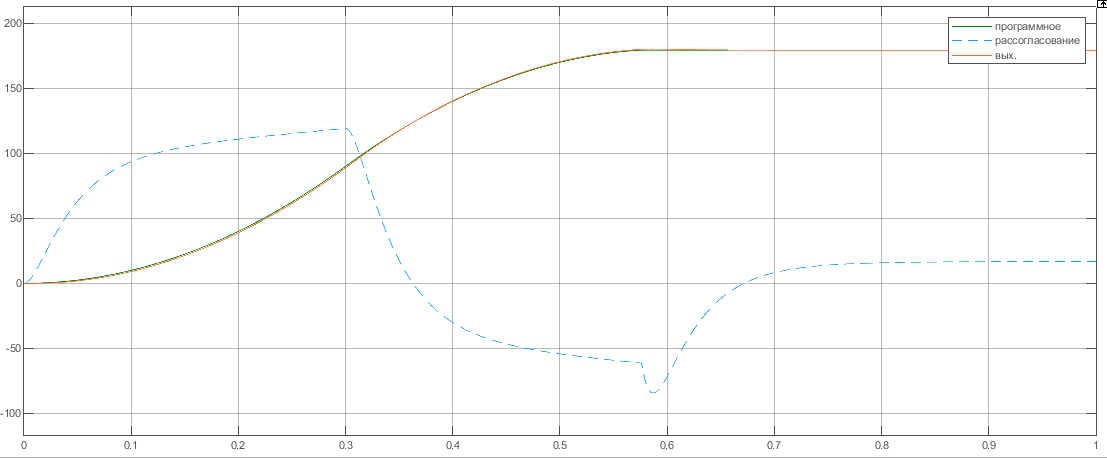
\includegraphics[width=1.0\linewidth]{az_digital3_saturation} 
	\caption{Процессы наведения ОЭП с учетом насыщения УМ}
	\label{fig:az_digital3}
\end{figure}

- при учете только ШИМ УМ ($f_g = 16000$ Гц) и насыщения УМ погрешность наведения существенно не изменилась ($\varDelta\alpha < 1.2^0$) (рисунок \ref{fig:az_digital4});\par

\begin{figure}
	\centering
	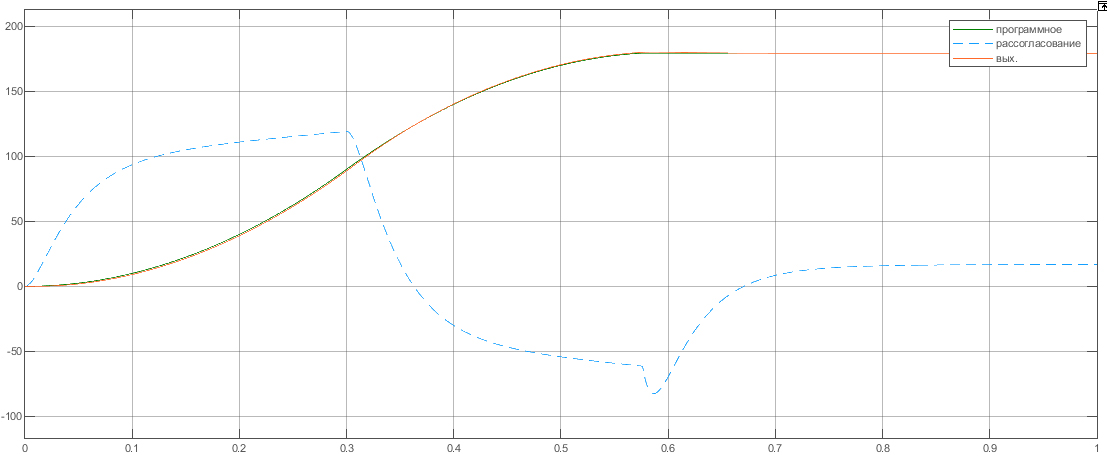
\includegraphics[width=1.0\linewidth]{az_digital4_pwm} 
	\caption{Процессы наведения ОЭП с учетом ШИМ УМ}
	\label{fig:az_digital4}
\end{figure}

- учет только дискретности датчика угла ($\varDelta_{\textit{ду}} = 1.3183 \textit{угл. мин} = 3.83 \cdot 10^{-4} \textit{рад}$) приводит к появлению пульсаций ($\varDelta\alpha_{\textit{пул}} < 0.08^0$) прибора из-за дискретности датчика угла, при этом погрешность наведения равна $\varDelta\alpha < 1.2^0$ (рисунок \ref{fig:az_digital5}).\par

\begin{figure}
	\centering
	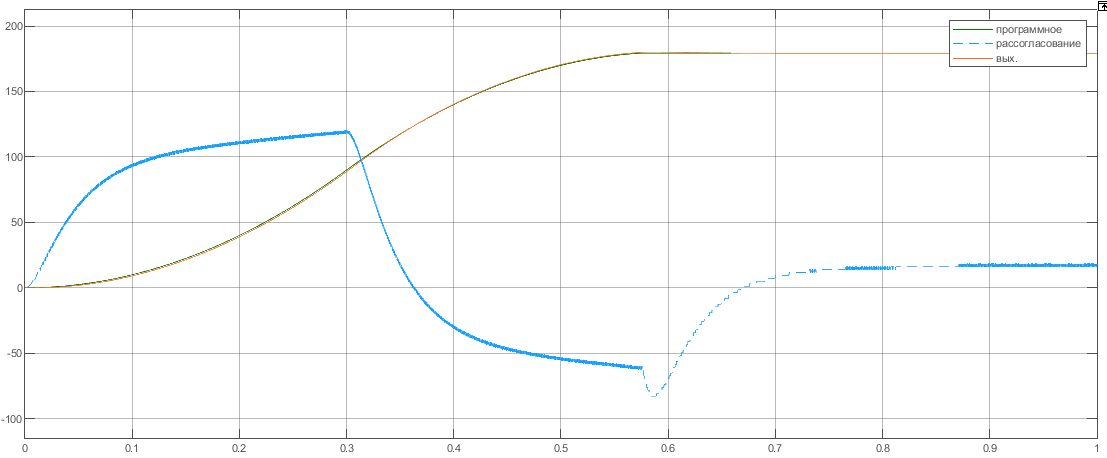
\includegraphics[width=1.0\linewidth]{az_digital5_sensor} 
	\caption{Процессы наведения ОЭП с учетом дискретности ДУ (14 разрядов)}
	\label{fig:az_digital5}
\end{figure}
- уменьшение времени разворота в ПУ до 0.5 секунд приводит к улучшению требуемых характеристик (рисунок \ref{fig:az_digital6})

\begin{figure}
	\centering
	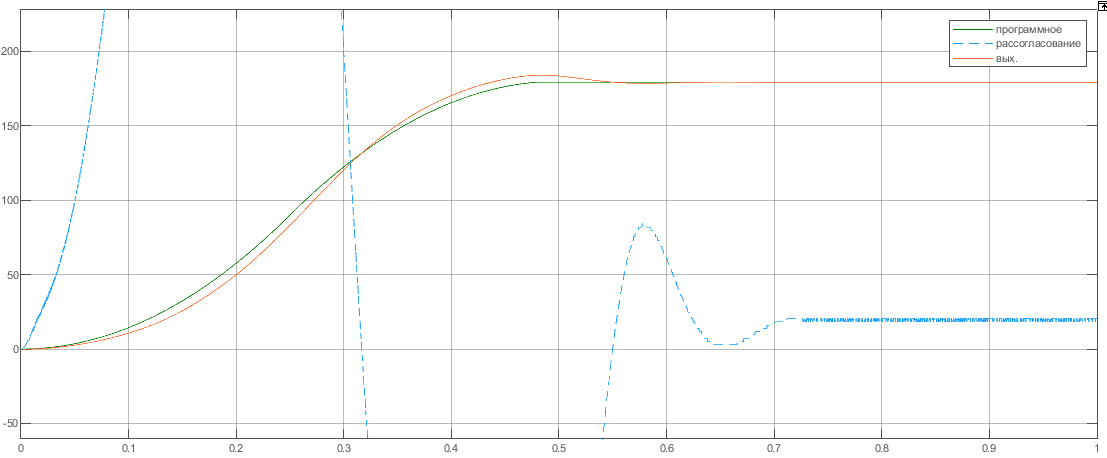
\includegraphics[width=1.0\linewidth]{az_digital6_05sec} 
	\caption{Процессы наведения ОЭП с корректировкой ПУ}
	\label{fig:az_digital6}
\end{figure}









\textbf{Угол места}


-при совместном учете насыщения УМ, дискретности ДУ и ШИМ УМ, погрешность наведения на угол $-60^0$ равна $\varDelta \beta = 0.6^0$ (рисунок \ref{fig:um_digital}).\par

\begin{figure}[ht]
	\centering
	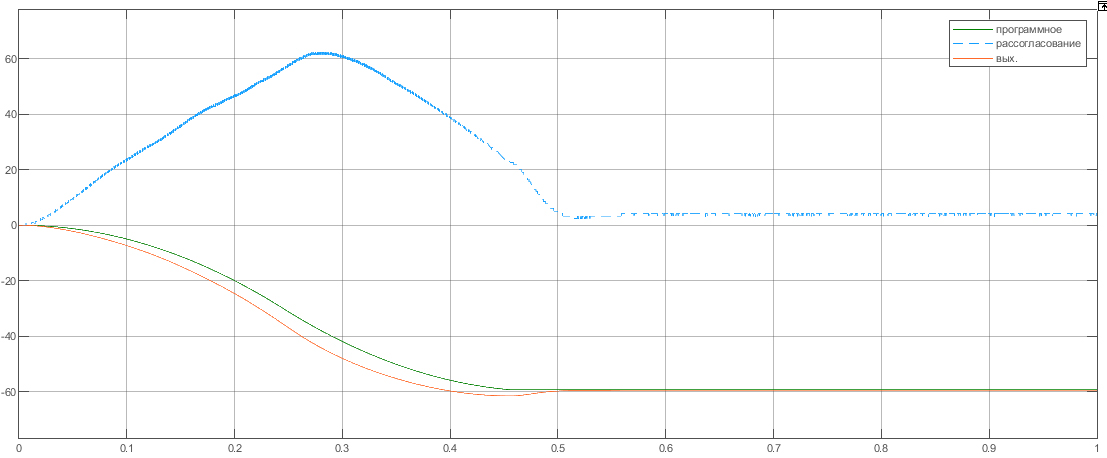
\includegraphics[width=1.0\linewidth]{um_digital1} 
	\caption{КИМ 3, Процессы наведения ОЭП с учетом насыщения УМ, дискретности ДУ и ШИМ УМ ($K_{\textit{д1}} K_{\textit{у1}} K_{\textit{к1}} = 150 \textit{В/рад}$)}
	\label{fig:um_digital}
\end{figure}

-При этом изменение напряжения на выходе УМ в процессе наведения приведены на рисунке ниже (рисунок \ref{fig:um_digital2}). Период переключений напряжений: ($0.12 \div 1.25$) мс.\par

\begin{figure}[ht]
	\centering
	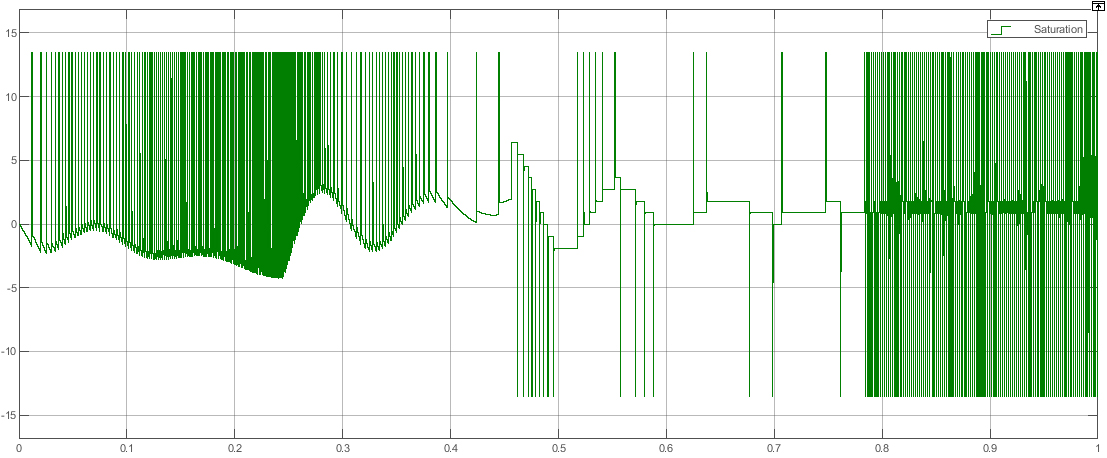
\includegraphics[width=1.0\linewidth]{um_digital2} 
	\caption{Изменение напряжения на выходе усилителя мощности в процессе наведения}
	\label{fig:um_digital2}
\end{figure}

- учет только насыщения УМ ($U_{max} = 27 \textit{В}$) приводит к увеличению времени переходного процесса, погрешность наведения достигает величины $\varDelta \beta = 0.65^0$ (рисунок \ref{fig:um_digital3}). При $K_{\textit{д1}} K_{\textit{у1}} K_{\textit{к1}} = 1000 \textit{В/рад}$ погрешность наведения можно уменьшить до величины  $\varDelta \beta = 0.46^0$. \par


\begin{figure}[ht]
	\centering
	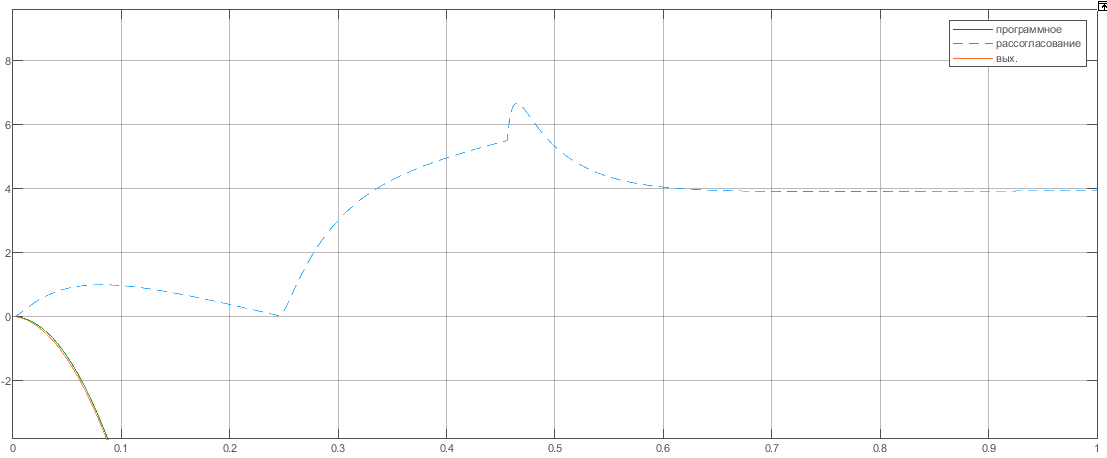
\includegraphics[width=1.0\linewidth]{um_digital3_saturation} 
	\caption{Процессы наведения ОЭП с учетом насыщения УМ}
	\label{fig:um_digital3}
\end{figure}

- при учете только ШИМ УМ ($f_y = 16000 \textit{Гц}$) и насыщения УМ погрешность наведения существенно не изменилась ($\varDelta \beta = 0.65^0$) (рисунок \ref{fig:um_digital4});\par

\begin{figure}[ht]
	\centering
	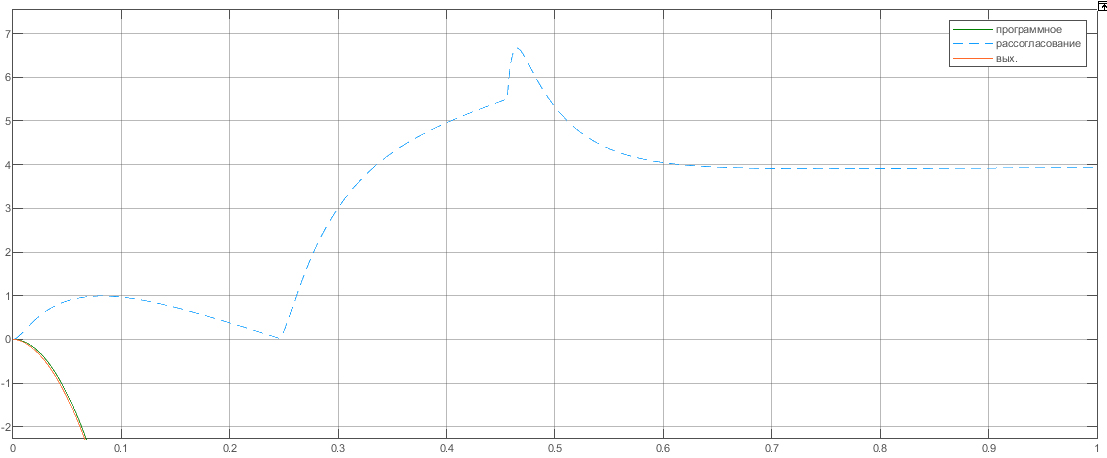
\includegraphics[width=1.0\linewidth]{um_digital4_pwm} 
	\caption{Процессы наведения ОЭП с учетом ШИМ УМ}
	\label{fig:um_digital4}
\end{figure}


- учет только дискретности датчика угла ($\varDelta_{\textit{ду}} = 1.3183 \textit{угл. мин} = 3.83 \cdot 10^{-4} \textit{рад}$) приводит к появлению пульсаций ($\varDelta \beta_{\textit{пул}} < 0.04^0$) прибора из-за дискретности датчика угла, при этом погрешность наведения равна $\varDelta \beta = 0.38$ (рисунок \ref{fig:um_digital5}).\par

\begin{figure}[ht]
	\centering
	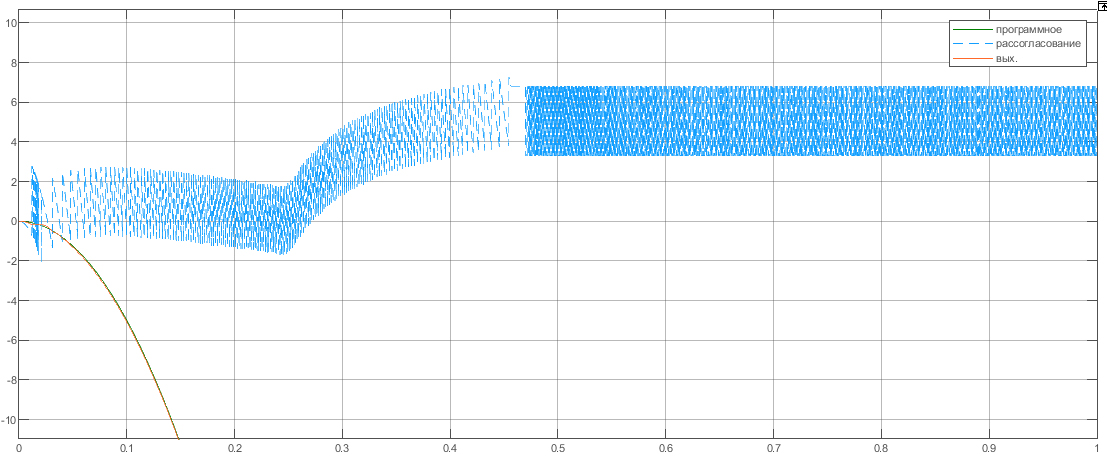
\includegraphics[width=1.0\linewidth]{um_digital5_sensor} 
	\caption{Процессы наведения ОЭП с учетом дискретности ДУ (14 разрядов)}
	\label{fig:um_digital5}
\end{figure}

\subsection{Моделирование и исследование динамики изолированных каналов управления ОЭП в режиме стабилизации} \label{ch:ch4/sect6}

Режим стабилизации ОЭП выполняется после режима наведения вокруг заданной координаты. В связи с этим рассмотрим возможность максимального использования регуляторов, синтезированных ранее для режима наведения, в режиме стабилизации. В этом режиме при действии возмущений, идущих от носителя, а также моментов трения и дисбаланса  объекта управления, оптическая ось прибора должна следить за объектом наблюдения с точностью $\varDelta \alpha = 30 \textit{угл. мин}$ в течении \textit{10 с}. Предполагаем, что в режиме стабилизации носитель может совершать эволюции, представленные в таблице \ref{tab:disturb}, 

\begin{table}[!h]
	\caption{Параметры эволюций носителя}%
	\label{tab:disturb}% label всегда желательно идти после caption
	\centering
	\begin{tabular}{p{0.23in}p{0.99in}p{0.82in}p{0.62in}p{0.18in}p{0.62in}p{0.16in}p{0.49in}p{0.7in}}
		\hline
		%row no:1
		\multicolumn{1}{|p{0.23in}}{№} & 
		\multicolumn{8}{|p{5.87in}|}{Гармонические возмущения} \\
		\hline
		%row no:2
		\multicolumn{1}{|p{0.23in}}{} & 
		\multicolumn{3}{|p{2.72in}}{Азимут} & 
		\multicolumn{5}{|p{2.95in}|}{Угол места} \\
		\hline
		%row no:3
		\multicolumn{1}{|p{0.23in}}{} & 
		\multicolumn{1}{|p{0.99in}}{Амплитуда (А), град} & 
		\multicolumn{1}{|p{0.82in}}{Период (Т), с} & 
		\multicolumn{1}{|p{0.62in}}{$\omega=2\pi/T$, \par 1/с} & 
		\multicolumn{2}{|p{1.0in}}{Амплитуда (А), град} & 
		\multicolumn{2}{|p{0.85in}}{Период (Т), с} & 
		\multicolumn{1}{|p{0.7in}|}{$\omega=2\pi/T$, \par 1/с} \\
		\hline
		%row no:4
		\multicolumn{1}{|p{0.23in}}{1} & 
		\multicolumn{1}{|p{0.99in}}{12} & 
		\multicolumn{1}{|p{0.82in}}{6.28} & 
		\multicolumn{1}{|p{0.62in}}{1} & 
		\multicolumn{2}{|p{1.0in}}{12} & 
		\multicolumn{2}{|p{0.85in}}{6,28} & 
		\multicolumn{1}{|p{0.7in}|}{1} \\
		\hline
		%row no:5
		\multicolumn{1}{|p{0.23in}}{2} & 
		\multicolumn{1}{|p{0.99in}}{2} & 
		\multicolumn{1}{|p{0.82in}}{1} & 
		\multicolumn{1}{|p{0.62in}}{6.28} & 
		\multicolumn{2}{|p{1.0in}}{2} & 
		\multicolumn{2}{|p{0.85in}}{1} & 
		\multicolumn{1}{|p{0.7in}|}{6.28} \\
		\hline
		%row no:6
		\multicolumn{1}{|p{0.23in}}{3} & 
		\multicolumn{1}{|p{0.99in}}{20} & 
		\multicolumn{1}{|p{0.82in}}{2} & 
		\multicolumn{1}{|p{0.62in}}{3.14} & 
		\multicolumn{2}{|p{1.0in}}{20} & 
		\multicolumn{2}{|p{0.85in}}{1} & 
		\multicolumn{1}{|p{0.7in}|}{6.28} \\
		\hline
		%row no:7
		\multicolumn{1}{|p{0.23in}}{4} & 
		\multicolumn{1}{|p{0.99in}}{20} & 
		\multicolumn{1}{|p{0.82in}}{1} & 
		\multicolumn{1}{|p{0.62in}}{6.28} & 
		\multicolumn{2}{|p{1.0in}}{20} & 
		\multicolumn{2}{|p{0.85in}}{1} & 
		\multicolumn{1}{|p{0.7in}|}{6.28} \\
		\hline
		%row no:8
		\multicolumn{1}{|p{0.23in}}{5} & 
		\multicolumn{1}{|p{0.99in}}{20} & 
		\multicolumn{1}{|p{0.82in}}{0.5} & 
		\multicolumn{1}{|p{0.62in}}{12.56} & 
		\multicolumn{2}{|p{1.0in}}{20} & 
		\multicolumn{2}{|p{0.85in}}{0.5} & 
		\multicolumn{1}{|p{0.7in}|}{12.56} \\
		\hline
		%row no:9
		\multicolumn{1}{|p{0.23in}}{} & 
		\multicolumn{8}{|p{5.87in}|}{Разворот с постоянной угловой скоростью. град/с} \\
		\hline
		%row no:10
		\multicolumn{1}{|p{0.23in}}{6} & 
		\multicolumn{2}{|p{2.0in}}{12} & 
		\multicolumn{2}{|p{0.91in}}{} & 
		\multicolumn{2}{|p{0.98in}}{} & 
		\multicolumn{2}{|p{1.39in}|}{12} \\
		\hline		
		
	\end{tabular}
\end{table}

Колебания носителя (варианты 1, 2 с частотами 0.16 Гц и 1Гц соответственно моделируют остаточные колебания САУ носителем) учитывались при исследовании САУ в режиме наведения как постоянно действующие возмущения. Поэтому в режиме стабилизации эти колебания будем также рассматривать как постоянно действующими возмущениями при всех других вариантах эволюций носителя.

Кроме того, при больших эволюциях ОЭП совместно с носителем ($\pm180^0$) исследование влияние дисбаланса на динамику управления будем проводить при исследовании пространственной модели объекта управления.


В отличие от САУ в режиме наведения (рисунок \ref{fig:structured_SAU}) структурная схема в режиме стабилизации будет иметь программное устройство с другим алгоритмом.

Исходные данные для расчета:

\begin{comment}
\begin{equation}
\label{eq:p4:425}
\begin{array}{ll}
\alpha_{\textit{вх1}}(t) = \psi_{01}(t) + \psi_{1}(t) + \psi_{2}(t),\\
\psi_{01}(t) =0.21 t, 
\psi_{1}(t) = 0.035 sin(6.28 t),
\psi_{2}(t) = 0.21 sin(t),\\
\alpha_{\textit{вх2}} = \psi_{0i}(t) + \psi_{1}(t) + \psi_{2}(t),\\
\psi_{0i}(t) = A_i sin(\omega_i t), (i=3,4,5),\\
\alpha_{\textit{вх}} =\alpha_{\textit{вх1}}+\alpha_{\textit{вх2}},\\
M_{\textit{тр}} = 0.08 sign( \dot \alpha ) \textit{Нм},\\
T_{M1} = 1.08 c, T_{e1} = 0.1 mc, T_{k1} = 0.05 c, T_{k2} = 0.5 mc,\\
K_{p1} = 3.7 \textit{рад/Вс}, K_{m1} = 3.29 \textit{рад/Нмс}, 
K_{с1} = 3700 \textit{с}^{-1},\\
K_{d1}K_{u1}K_{k1} = 1000 \textit{В/рад},\\
U_{max} = \pm 27 \textit{В}, \varDelta_{\textit{ду}} = 1.3183 \textit{угл.мин}, 
f_y = 16 \textit{кГц}
\end{array}
\end{equation}
 kkkkkkk
\end{comment}

\begin{equation}
 \label{eq:p4:425+}
 \begin{array}{ll}
 q_{\textit{вх}}(t) = \Omega_{01}(t) + \Omega_{1}(t) + \Omega_{2}(t),\\
 \Omega_{01}(t) = e_2\cdot 0.21 t, 
 \Omega_{1}(t) = e_2\cdot 0.035 sin(6.28 t),
 \Omega_{2}(t) = e_2\cdot 0.21 sin(t),\\
 q_{\textit{вх2}} = \Omega_{0i}(t) + \Omega_{1}(t) + \Omega_{2}(t),\\
 \Omega_{0i}(t) = \left( \begin{array}{c}
 {A^\psi}_i sin({\omega^\psi}_i t)  \\
 {A^\vartheta}_i sin({\omega^\vartheta}_i t) 
 \end{array}\right)
 , (i=3,4,5),\\
 q_{\textit{вх}} = q_{\textit{вх1}}+ q_{\textit{вх2}},\\
 M_{\textit{тр}}(q) = M_{\textit{тр}} sign( \dot q ) \textit{Нм} = ,\\
 T_{M} = \left( \begin{array}{c c}
 1.08 & 0 \\
 0 & 0.29
 \end{array}\right) c, 
 T_{e} = \left( \begin{array}{c c}
 0.1 &0  \\
 0&0.4
 \end{array}\right) mc,\\
 T_{k1} = e_2\cdot 0.05 \ c, T_{k2} = e_2\cdot 0.05 \ mc \ (\ref{eq:p4:xx}),\\
 K_{n} = \left( \begin{array}{c c}
 3.7&0  \\
 0&8.33
 \end{array}\right) \textit{рад/Вс}, 
 K_{m} = \left( \begin{array}{c c}
 3.29&0  \\
 0&33.68
 \end{array}\right) \textit{рад/Нмс} (\ref{eq:p4:sec4/4},\ \ref{eq:p4:sec4/4+}),\\ 
 K_{c} = \left( \begin{array}{c c}
 3700&0  \\
 0&3000
 \end{array}\right) \textit{с}^{-1},
 K_{\textit{д}}K_{\textit{у}}K_{k} = \left( \begin{array}{c c}
 1000&0  \\
 0&360
 \end{array}\right) \textit{В/рад},\\
 U_{max} = \pm 27 \textit{В}, \varDelta_{\textit{ду}} = 1.3183 \textit{угл.мин}, 
 f_y = 16 \textit{кГц}
 \end{array}
\end{equation}

Дополним систему уравнений (\ref{eq:p4:414}) принятыми ранее нелинейностями и представим в виде новой системы уравнений:

\begin{equation}%\tag{414}
\label{eq:p4:426+}
\begin{alignedat}{2}
\left. \begin{array}{ll}
q = W_n(p) \overline u - W_f(p) M_{\textit{н}} - W_{\textit{ла}} (p)\omega\\
\Delta  q = q_{\textit{пр}}- \widetilde q\\
\widetilde q = \mu (  q  ) \\
\overline u = F ( \widetilde u)\\
\widetilde u = f (u)\\
u = K_{\textit{д}}\cdot K_{y} \cdot W_{k} \left( p \right)  \Delta  q \\
\end{array}  \right\rbrace  
\end{alignedat}
\end{equation}

где 
$F(\widetilde{u})=K_F(\widetilde{u})\widetilde{u}$ - нелинейная функция насыщения УМ ($\pm 27$ В),

$f(u)=K_f(u)u$ - нелинейная функция ШИМ УМ ($f_{\textit{y}} = 16 \textit{кГц}$),

$\mu(q)=K_\mu(q)q$ - нелинейная функция дискретизации цифрового ДУ ($\Delta_{\textit{ду}} = 1.3183$ угловых минут).

Из линеаризованных уравнений (\ref{eq:p4:426+}) получим ПФ по ошибке

\begin{equation}%\tag{415}
\label{eq:p4:427-}
\begin{alignedat}{2}
\Delta  q = 
(\overline W(p)+E_2)^{-1} q _{\textit{пр}}-
(\overline W(p)+E_2)^{-1} \overline W_{f1} \left( p \right) M_{H}-\\
(\overline W(p)+E_2)^{-1} \overline W_{\textit{ла}} (p) (\Omega_{1}(t) + \Omega_{2}(t)),
\end{alignedat}
\end{equation}

где
\begin{equation}
\label{eq:p4:427-+}
\begin{array}{ll}
\overline W (p) = K_\mu(q) W_n(p) K_F(\widetilde{u}) K_f(u) K_{\textit{д}}\cdot K_{y} \cdot W_{k} \left( p \right) = \overline K_c W_n(p) W_{k} ( p ) K_k^{-1},\\
\overline W_{f1} (p) = K_\mu(q) W_{f1} (p),\\ 
\overline W_{\textit{ла}} (p) = K_\mu(q) W_{\textit{ла}} (p)
\end{array}
\end{equation}

из которой следует (как и в линейной системе), что погрешность стабилизации зависит от трех составляющих: угловой скорости входного сигнала, момента нагрузки и ускорений колебаний носителя.

В установившемся режиме ($t \longrightarrow 0, p \longrightarrow 0$) имеем\par

\begin{equation}
\label{eq:p4:428+}
\begin{alignedat}{2}
\Delta  q =
\overline K_{c}^{-1} \dot q_{\textit{пр}} + 
K_{m} \overline K_{c}^{-1} M_{\textit{н}} - 
T_{m} \overline K_{c}^{-1} (\Omega_{1}(t) + \Omega_{2}(t))
\end{alignedat}
\end{equation}

При заданных исходных данных, соответствующих регулятору САУ в режиме наведения по азимуту, разработана КИМ 5  (рисунок 4.29), включающая в себя новую модель входных воздействий (\ref{eq:p4:425+}), измененные параметры нелинейностей ($\Delta_{\textit{ду}} = 1.3183$ угловых минут, $f_{\textit{y}} = 16 \textit{кГц}$), линейная и нелинейная части САУ в соответствии с системой уравнений (\ref{eq:p4:426+}).\par

Разработанная КИМ САУ для режима стабилизации (рисунок 4.29) позволяет проводить исследования динамики процесса управления ОЭП, варьируя параметрами регулятора, объекта управления и возмущающими воздействиями в широких пределах в соответствии с исходными данными (\ref{eq:p4:425+}) и таблицей \ref{tab:disturb}.\par

рисунок модели 

\subsubsection{Моделирование и исследование динамики нелинейной САУ по азимуту} \label{subsec:ch4/sect6/sub1}

\begin{comment}
Уравнения движения системы с учетом 46,47,(\ref{eq:p4:414}) и принятых ранее нелинейностей представим в виде :\par

\begin{equation}
\label{eq:p4:426}
\begin{alignedat}{2}
\left. \begin{array}{ll}
\alpha =W_{n1} \left( p \right) \overline{U}_{1}-W_{f1} \left( p \right) M_{H1}-W_{ \psi } \left( p \right) \dot \psi \\
\overline{U}_{1}=F_{1} \left( \widetilde{U}_{1} \right) \\
\widetilde{U}_{1}=f_{1} \left( U_{1} \right) \\
U_{1}=K_{\textit{у1}} \cdot W_{k1} \left( p \right) U_{\textit{д1}} \\
U_{\textit{д1}}=K_{\textit{д1}} \cdot \Delta \alpha \\
\Delta  \alpha = \alpha _{\textit{вх}}- \widetilde \alpha \\
\widetilde \alpha = \mu _{1} \left(  \alpha  \right) \\
\end{array}  \right\rbrace  
\end{alignedat}
\end{equation}

где 
$F_{1}(\widetilde{U}_{1})$ - нелинейная функция насыщения УМ ($\pm 27$ В),

$f_{1}(U_{1})$ - нелинейная функция ШИМ УМ ($f_{\textit{y}} = 16 \textit{кГц}$),

$\mu_{1}(\alpha)$ - нелинейная функция дискретизации цифрового ДУ ($\Delta_{\textit{ду}} = 1.3183$ угловых минут).

Из линеаризованных уравнений (\ref{eq:p4:426}) получим ПФ по ошибке

\begin{equation}
\label{eq:p4:427}
\Delta  \alpha =
\frac{1}{1+W_{1} \left( p \right) } \alpha _{\textit{вх}} - 
\frac{W_{f1} \left( p \right) }{1+W_{1} \left( p \right) }M_{\textit{тр1}} - 
\frac{W_{ \psi } \left( p \right) }{1+W_{1} \left( p \right) } \left(  \dot\psi _{1}+ \dot \psi _{2} \right) 
\end{equation}

где
\begin{equation}
\label{eq:p4:427+}
\begin{array}{ll}
W_{1} \left( p \right) = K_{\textit{д1}} \mu_{1}(\alpha) K_{\textit{у1}} f_1(U_1) F_{1}(\widetilde{U}_{1}) W_{k1} (p) = W_{k1} (p) \frac{K_{C1} K_{\textit{н1}}}{(T_{m1} T_{e1} p^2 + T_{m1} p + 1)p},\\
\overline K_{C1} = K_{C1} K_{\textit{к1}} K_{\textit{н1}}, K_{C1} = K_{\textit{д1}},\\ K_{\textit{у1}} K_{\textit{n1}},\\
K_{\textit{н1}} = K_{\mu 1} K_{f1} K_{F1},\\
W_{ \psi 1 } \left( p \right) = \frac{T_{m1} (T_{e1} p +1)}{(T_{m1} T_{e1} p^2 + T_{m1} p + 1)},\\
W_{f1} \left( p \right) =  \frac{K_{m1} (T_{e1} p +1)}{(T_{m1} T_{e1} p^2 + T_{m1} p + 1) p}
\end{array}
\end{equation}

$K_{\textit{н1}}$ - линеаризованные коэффициенты нелинейностей,

из которой следует (как и в линейной системе), что погрешность стабилизации зависит от трех составляющих: угловой скорости входного сигнала, момента нагрузки и ускорений колебаний носителя.

В установившемся режиме ($t \longrightarrow 0, p \longrightarrow 0$) имеем\par


\begin{equation}%\tag{428}
\label{eq:p4:428}
\Delta  \alpha =
\frac{1}{\overline K_{C1}} \dot \alpha _{\textit{вх}} -
\frac{K_{M1}}{\overline K_{C1}}M_{\textit{тр1}}-
\frac{T_{M}}{\overline K_{C1}} ( \dot \psi_{1} + \dot \psi_{2}),
\end{equation}
При заданных исходных данных, соответствующих регулятору САУ в режиме наведения по азимуту, разработана КИМ 5  (рисунок 4.29), включающая в себя новую модель входных воздействий (\ref{eq:p4:425}), измененные параметры нелинейностей ($\Delta_{\textit{ду}} = 1.3183$ угловых минут, $f_{\textit{y}} = 16 \textit{кГц}$), линейная и нелинейная части САУ в соответствии с системой уравнений (\ref{eq:p4:426}).\par

Разработанная КИМ САУ для режима стабилизации (рисунок 4.29) позволяет проводить исследования динамики процесса управления ОЭП, варьируя параметрами регулятора, объекта управления и возмущающими воздействиями в широких пределах в соответствии с исходными данными (\ref{eq:p4:425}) и таблицей \ref{tab:disturb}.\par

\end{comment}

На рисунках 4.30 - 4.32 приведены переходные и установившиеся процессы стабилизации ОЭП относительно заданного направления при действии указанных выше возмущений и нелинейностей (\ref{eq:p4:425+}). При этом коэффициенты датчика и усилителя должны быть не менее $K_{\textit{д1}} K_{\textit{к1}} K_{\textit{у1}} = 1000$ В/рад.

Из анализа полученных процессов управления ОЭП по азимуту следует:

\begin{enumerate}
	\item при развороте носителя с постоянной угловой скоростью  $\alpha_{\textit{вх1}}(t)$ (\ref{eq:p4:425+}) по азимуту процессы управления ОЭП приведены на рис.31, где погрешность стабилизации не превышает  $\varDelta\alpha=0.18$ град,
	\item при гармонических колебаниях носителя по азимуту
	
	\begin{equation}
	\label{eq:p4:429}
	\psi_{1}(t)=0.035sin(6.28t),\psi_{2}(t)=0.21sin(t),
	\end{equation}
	
	погрешность стабилизации равна $\varDelta\alpha=0.17$ (Рисунок 4.31),
	
	сунок 4.30. Рис.31 Процессы стабилизации ОЭП при действии вх1 (t) (вариант 6):
	
	\textsubscript{вх2} – входное управление,  - угол отработки входного воздействия,
	- погрешность стабилизации,  - угловая скорость\  привода.
	
	сунок 4.31. Рис.32 Процессы стабилизации ОЭП при действии вх1 (t) (варианты:1+2):
	
	\textsubscript{вх1} – входное управление,  - угол отработки входного воздействия,\ 
	- погрешность стабилизации,  - угловая скорость привода.
	
	\item при колебаниях носителя с амплитудой 20 град. и частотой 0,5 Гц  совместно с колебаниями 429 погрешность стабилизации равна  =0,4 град. (Рисунок 4.32),
	
	сунок 4.32.Рис.33 Процессы стабилизации ОЭП при действии вх2 (t) (вариант 3):
	
	\textsubscript{вх2} – входное управление,  - угол отработки входного воздействия,\ - погрешность стабилизации,  - угловая скорость привода. 
	
	\item при остальных колебаниях носителя с амплитудами 20 град. с частотами 1 и  2  Гц (варианты 4 и 5) совместно с колебаниями  429 система управления не справляется с этими возмущениями из-за больших инерционных моментов ( \( J_{1} \psi _{4} \left( t \right)  \)  и  \( J_{1} \psi _{5} \left( t \right)  \) ). При снижении  момента инерции первого тела в два раза погрешность стабилизации на частоте  1 Гц будет составлять   =1,3 град, при снижении момента инерции первого тела на 30 $\%$  погрешность стабилизации на частоте 1Гц будет равна     =3  град.
\end{enumerate}


\subsubsection{Моделирование и исследование динамики нелинейной САУ по углу места} \label{subsec:ch4/sect6/sub2}


На рисунках далее (Рисунок 4.35 - Рисунок 4.39) приведены переходные и установившиеся процессы стабилизации ОЭП относительно заданного направления с учетом указанных выше возмущений (эволюций носителя) и нелинейностей 430. При этом коэффициенты датчика и усилителя К\textsubscript{д2 }К\textsubscript{к2} К\textsubscript{у2}\textit{= }360 В/рад. \par

Из анализа процессов управления ОЭП по углу места следует:\par

\begin{enumerate}
	\item при развороте носителя с постоянной угловой скоростью \textsubscript{вх1}(t) 430 процессы управления приведены на рис.36, где погрешность стабилизации ОЭП не превышает  =0,2 град\textit{. }
	
	сунок 4.35. Рис.36. Процессы стабилизации ОЭП при действии вх1(t) (вариант 6) :
	
	\textsubscript{вх1} – входное управление,  - угол отработки входного воздействия,- погрешность стабилизации,  - угловая скорость\  привода.
	
	\item при гармонических колебаниях носителя по углу места \textsubscript{1}(t) и \textsubscript{2}(t) 
	
	\begin{equation}
	\label{eq:p4:433}
	\vartheta_{1}(t)=0.035sin(6.28t),\vartheta_{2}(t)=0.21sin(t),
	\end{equation}
	
	погрешность стабилизации равна  =0,15 град. (Рисунок 4.36),
	
	сунок 4.36. Рис.37. Процессы стабилизации ОЭП при действии вх1(t) (варианты:1+2):
	\textsubscript{вх1} – входное управление,  - угол отработки входного воздействия,- погрешность стабилизации,  - угловая скорость\  привода.
	
	\item при колебаниях носителя с амплитудой 20 град. и частотой 1 Гц  совместно с колебаниями 433 погрешность стабилизации равна  =0,4 град. (Рисунок 4.37),
	
	сунок 4.37. Рис.38. Процессы стабилизации ОЭП при действии вх2(t) (вариант3,4):\textsubscript{вх2} – входное управление,  - угол отработки входного воздействия,- погрешность стабилизации,  - угловая скорость\  привода.
	
	\item при  колебаниях носителя с амплитудой 20 град. и частотой 2  Гц (вариант 5) совместно с колебаниями 423 погрешность стабилизации превышает допустимую величину в три раза –   =1,5 град (Рисунок 4.39), для обеспечения требований ТЗ добротность по скорости регулятора необходимо увеличить в 3 раза ( К\textsubscript{с2}=9000 с\textsuperscript{-1}, К\textsubscript{д2 }К\textsubscript{к2} К\textsubscript{у2}=\textit{ }1080 \textit{В/рад}) (Рисунок 4.40).
	
	сунок 4.38. Рис.39. Процессы стабилизации ОЭП при действии вх2(t) (вариант5):	\textsubscript{вх2} – входное управление,  - угол отработки входного воздействия,- погрешность стабилизации,  - угловая скорость\  привода.
	
	сунок 4.39. Рис.40. Процессы стабилизации ОЭП при действии вх2(t) (вариант5):\textsubscript{вх2} – входное управление,  - угол отработки входного воздействия,- погрешность стабилизации,  - угловая скорость\  привода.
\end{enumerate}


\section{Анализ результатов исследований и определение требований к элементам САУ} \label{ch:ch4/sect7}

В результате проведенных исследований динамики изолированных каналов управление ОЭП разработаны в соответствии с уравнениями 413414420421426431 КИМ 7 САУ по азимуту (Рисунок 4.40) и КИМ 8 САУ углу места (Рисунок 4.41), позволяющие получать процессы управления в заданных режимах управления  ОЭП и отыскивать при этом приемлемые параметры регулятора ( К\textsubscript{с}, К\textsubscript{п}, К\textsubscript{м},Т\textsubscript{м}, Т\textsubscript{э}, Т\textsubscript{к}) и объекта управления\ в режимах наведения и стабилизации, которые реализуются с помощью переключателя  5 (Manual Switch5)\ путем подачи на вход  САУ программного управления (режим наведения) и входных воздействий (режим стабилизации).\par

В таблицах ниже (Таблица 4.4, Таблица 4.5) сведены результаты исследования, полученные в разделах 4.4.1,4.5,4.6.

%%%%%%%%%%%%%%%%%%%% Table No: 14 starts here %%%%%%%%%%%%%%%%%%%%


\begin{table}[H]
	\centering
	\begin{tabular}{p{1.37in}p{1.47in}p{1.41in}p{1.24in}}
		\hline
		%row no:1
		\multicolumn{1}{|p{1.37in}}{Параметры} & 
		\multicolumn{1}{|p{1.47in}}{Максимальная  \par скорость, град/с} & 
		\multicolumn{1}{|p{1.41in}}{Угол \par наведения, град.} & 
		\multicolumn{1}{|p{1.24in}|}{Погрешность \par наведения} \\
		\hhline{----}
		%row no:2
		\multicolumn{1}{|p{1.37in}}{САУ по азимуту} & 
		\multicolumn{1}{|p{1.47in}}{599,93} & 
		\multicolumn{1}{|p{1.41in}}{180} & 
		\multicolumn{1}{|p{1.24in}|}{0,2\textsuperscript{0}} \\
		\hhline{----}
		%row no:3
		\multicolumn{1}{|p{1.37in}}{САУ по УМ} & 
		\multicolumn{1}{|p{1.47in}}{299,94} & 
		\multicolumn{1}{|p{1.41in}}{90} & 
		\multicolumn{1}{|p{1.24in}|}{0,023\textsuperscript{0}} \\
		\hhline{----}
		
	\end{tabular}
\end{table}


%%%%%%%%%%%%%%%%%%%% Table No: 14 ends here %%%%%%%%%%%%%%%%%%%%


%%%%%%%%%%%%%%%%%%%% Table No: 15 starts here %%%%%%%%%%%%%%%%%%%%


\begin{table}[H]
	\centering
	\begin{tabular}{p{1.28in}p{1.47in}p{1.08in}p{1.67in}}
		\hline
		%row no:1
		\multicolumn{4}{|p{6.1in}|}{\tab САУ по азимуту} \\
		\hhline{----}
		%row no:2
		\multicolumn{1}{|p{1.28in}}{Параметры \par возмущения} & 
		\multicolumn{1}{|p{1.47in}}{\textsubscript{0 } \par амплитуда, град.} & 
		\multicolumn{1}{|p{1.08in}}{f \par частота, Гц} & 
		\multicolumn{1}{|p{1.67in}|}{погрешность, град. \par } \\
		\hhline{----}
		%row no:3
		\multicolumn{1}{|p{1.28in}}{Варианты 1+2} & 
		\multicolumn{1}{|p{1.47in}}{1-12\  2-2} & 
		\multicolumn{1}{|p{1.08in}}{0,36} & 
		\multicolumn{1}{|p{1.67in}|}{0,17} \\
		\hhline{----}
		%row no:4
		\multicolumn{1}{|p{1.28in}}{Вариант 3} & 
		\multicolumn{1}{|p{1.47in}}{20} & 
		\multicolumn{1}{|p{1.08in}}{0,5} & 
		\multicolumn{1}{|p{1.67in}|}{0,4} \\
		\hhline{----}
		%row no:5
		\multicolumn{1}{|p{1.28in}}{Вариант 6} & 
		\multicolumn{1}{|p{1.47in}}{12} & 
		\multicolumn{1}{|p{1.08in}}{} & 
		\multicolumn{1}{|p{1.67in}|}{0,18} \\
		\hhline{----}
		%row no:6
		\multicolumn{1}{|p{1.28in}}{Варианты 4,5} & 
		\multicolumn{1}{|p{1.47in}}{20} & 
		\multicolumn{1}{|p{1.08in}}{1, 2} & 
		\multicolumn{1}{|p{1.67in}|}{более 10} \\
		\hhline{----}
		
	\end{tabular}
\end{table}


%%%%%%%%%%%%%%%%%%%% Table No: 15 ends here %%%%%%%%%%%%%%%%%%%%



%%%%%%%%%%%%%%%%%%%% Table No: 16 starts here %%%%%%%%%%%%%%%%%%%%


\begin{table}[H]
	\centering
	\begin{tabular}{p{1.37in}p{1.47in}p{1.18in}p{1.47in}}
		\hline
		%row no:1
		\multicolumn{4}{|p{6.1in}|}{\Centering САУ по углу места} \\
		\hhline{----}
		%row no:2
		\multicolumn{1}{|p{1.37in}}{Параметры возмущения} & 
		\multicolumn{1}{|p{1.47in}}{\textsubscript{0}  \par амплитуда, град.} & 
		\multicolumn{1}{|p{1.18in}}{f \par частота, Гц} & 
		\multicolumn{1}{|p{1.47in}|}{погрешность, град \par } \\
		\hhline{----}
		%row no:3
		\multicolumn{1}{|p{1.37in}}{Варианты 1+1} & 
		\multicolumn{1}{|p{1.47in}}{\Centering 1-12\  (2-2)} & 
		\multicolumn{1}{|p{1.18in}}{\Centering 0,36\  (1)} & 
		\multicolumn{1}{|p{1.47in}|}{\Centering 0,15} \\
		\hhline{----}
		%row no:4
		\multicolumn{1}{|p{1.37in}}{Варианты 3,4} & 
		\multicolumn{1}{|p{1.47in}}{\Centering 20} & 
		\multicolumn{1}{|p{1.18in}}{\Centering 1} & 
		\multicolumn{1}{|p{1.47in}|}{\Centering 0,4} \\
		\hhline{----}
		%row no:5
		\multicolumn{1}{|p{1.37in}}{Вариант 4} & 
		\multicolumn{1}{|p{1.47in}}{\Centering 20} & 
		\multicolumn{1}{|p{1.18in}}{\Centering 1} & 
		\multicolumn{1}{|p{1.47in}|}{\Centering 0,4} \\
		\hhline{----}
		%row no:6
		\multicolumn{1}{|p{1.37in}}{Вариант 5} & 
		\multicolumn{1}{|p{1.47in}}{\Centering 20} & 
		\multicolumn{1}{|p{1.18in}}{\Centering 0,5} & 
		\multicolumn{1}{|p{1.47in}|}{\Centering 1,5(0,5\textsuperscript{$\ast$ })} \\
		\hhline{----}
		%row no:7
		\multicolumn{1}{|p{1.37in}}{Вариант 6} & 
		\multicolumn{1}{|p{1.47in}}{\Centering 12} & 
		\multicolumn{1}{|p{1.18in}}{\Centering -} & 
		\multicolumn{1}{|p{1.47in}|}{\Centering 0,2} \\
		\hhline{----}
		
	\end{tabular}
\end{table}


%%%%%%%%%%%%%%%%%%%% Table No: 16 ends here %%%%%%%%%%%%%%%%%%%%
Погрешность 0,5\textsuperscript{0} достигается при К\textsubscript{с2}=9000 с\textsuperscript{-1}

На основе проведенных исследований динамики изолированных каналов управления ЦСАУ определ\colorbox{Yellow}{ены} требования к параметрам элементов регулятора и объекта управления из условий обеспечения точности управления, устойчивости и качества переходного процесса.\par

Для достижения требований ТЗ необходимо обеспечить дополнительные требования:

\begin{enumerate}
	\item 
	\item 
	\item 
	\item 
	\item 
	\item 
	\item 
\end{enumerate}





\section{Выводы по главе} \label{ch:ch4/sect8}

По результатам исследования динамики изолированных каналов управления ОЭП можно сделать следующие выводы:

\begin{enumerate}
	\item 
	\item 
	\item
	\item
	\item
	\item
	\item
	\item
	\item
\end{enumerate}




Некоторый текст.

\clearpage           % Глава 4
\chapter{Разработка КИМ пространственной модели и исследование динамики управления ОЭП при действии возмущений} \label{ch:ch5}

\section{КИМ трехфазного моментного привода} \label{ch:ch5/sect1}

5.1  
\section{КИМ САУ ОЭП (схема, обозначения и…) } \label{ch:ch5/sect2}

\section{Разработка компьютерной имитационной модели ЦСАУ ОЭП с учетом  движения борта} \label{ch:ch5/sect3}

\section{Исследование динамики наведения и стабилизации ОЭП} \label{ch:ch5/sect4}

\section{Выводы} \label{ch:ch5/sect5}
	


Некоторый текст.

\clearpage           % Глава 5
\include{Dissertation/conclusion}      % Заключение
\chapter*{Список сокращений и условных обозначений} % Заголовок
\addcontentsline{toc}{chapter}{Список сокращений и условных обозначений}  % Добавляем его в оглавление
\noindent
%\begin{longtabu} to \dimexpr \textwidth-5\tabcolsep {r X}
\begin{longtabu} to \textwidth {r X}
% Жирное начертание для математических символов может иметь
% дополнительный смысл, поэтому они приводятся как в тексте
% диссертации

\textbf{БОЭП} & бортовая оптико-электронная система \label{acroAEOS}\\

\textbf{СС} & Следящая система  \\

\textbf{ОЭП (ОЭС)} & Оптико-электронные приборы и системы \label{acroEOS}\\

\textbf{КИМ} & компьютерная имитационная модель \label{acroCSM} \\

\textbf{АЧХ (АФЧХ)} & Амплитудно-частотно фазовая характеристика \\

\textbf{ЧХ} & Частотная характеристика \\

\textbf{СА} & система амортизации \\

\textbf{САФ} & система автоматической фокусировки \\

\textbf{МК} & микроконтроллер \\

\textbf{ПЛИС} & программируемая логическая интегральная схема \\

\textbf{ФПУ} & фотоприёмное устройство (матрица) \\

\textbf{ДУС} & датчик угловых скоростей \\
\textbf{ДУП} & датчик углового положения (Энкодер) \label{acroDUP} \\

\textbf{ДТВ} & датчик телевизионный \\

\textbf{ГСН} & головкой самонаведения \label{acroGSN} \\

\textbf{ИБ} & измерительный блок \\

\textbf{БВМ} & бортовой вычислительная машина \\

\textbf{УМ} & усилитель мощности \\

\textbf{ВЧК} & модель высокочастотных колебаний \\

\textbf{ИИ} & источник излучения \\

\textbf{ИК} & инфракрасный \\

\textbf{ИМ} & имитационная модель \\

\textbf{КИ} & качество изображения \\

\textbf{КИМ} & компьютерная имитационная модель \\

\textbf{КМ} & компьютерная модель \\

\textbf{ЛА} & летательный аппарат \label{acroLA} \\

\textbf{ММ} & математическая модель \\

\textbf{МФП} & матричный фотоприемник \\

\textbf{НЧД} & модель низкочастотного движения \\

\textbf{НУТВ} & телевизионный \\

\textbf{ОН} & объект наблюдения \label{acroON}\\

\textbf{ОПФ} & оптическая передаточная функция \\

\textbf{ОС} & оптическая система \\

\textbf{ОУ} & объект управления \\

\textbf{ОЭК} & оптико-электронный комплекс \\

\textbf{ОЭС} & оптико-электронная система \\

\textbf{ПЗС} &прибор с зарядовой связью \\

\textbf{ПЗРК} & пусковой зенитный ракетный комплекс \\

\textbf{ПИД} & пропорционально-интегрально-дифференциальный \\

\textbf{ПСт} & система прецизионной стабилизации \\

\textbf{САУ} & система автоматического управления \label{acroSAU}\\

\textbf{САФ} & система автоматической фокусировки \\

\textbf{СВ} & система виброзащиты \\

\textbf{СКИ} & системы обеспечения качества изображения \\

\textbf{СОЭП} & система оптико-электронного подавления  \label{acroSOEP} \\

\textbf{ССк} & система сканирования \\

\textbf{ССл} & система слежения \\

\textbf{СТР} & система терморегулрования \\

\textbf{ТЗ} & техническое задание \label{acroTZ} \\

\textbf{ТС}  & телевизионная система \label{acroTS} \\

\textbf{УВ} & устройство визуализации \\

\textbf{УР} & управляемая ракета \\

\textbf{УПУ} & усилительно-преобразовательное устройство \\

\textbf{ЦСУ} & цифровая система управления \\

\textbf{ФКЯ} & фотоприемник на квантовых ямах \\

\textbf{ФПМ} & функция передачи модуляции \label{acroFPM}\\

\textbf{ФЦО} & фоноцелевая обстановка \\

\textbf{ТВС} & тепловизионной системы \label{acroTVS} \\

\textbf{ФС} & фотографической системы \label{acroFS} \\

\textbf{НИР} & научно исследовательской работы \label{acroNIR} \\

\textbf{БЛА} & беспилотные летательные аппараты \label{acroUAV} \\

\textbf{ПВО} & средства противовоздушной обороны \label{acroPVO} \\

\textbf{ТТХ} &  тактико технические требования \label{acroTTX} \\

\textbf{ТП} & технического предложения \\

\textbf{КД} & конструкторской документации \\

\textbf{НАТО} & Североатлантический Альянс \label{acroNATO}\ \\

\textbf{СВ} & вооруженных сил \\

\textbf{ВМС} & военно-морских сил \\

\textbf{ЦУ} & целеуказания  \\

\textbf{ТпВ} & тепловизор \\

\textbf{GPS} & система глобального позиционирования \\

\textbf{ЭВМ} &  электронно вычислительная машина \\

\textbf{БИзОЭП} &  бортовой излучающей оптико-электронной системы () \\


\end{longtabu}
\addtocounter{table}{-1}% Нужно откатить на единицу счетчик номеров таблиц, так как предыдующая таблица сделана для удобства представления информации по ГОСТ
        % Список сокращений и условных обозначений
\chapter*{Словарь терминов}             % Заголовок
\addcontentsline{toc}{chapter}{Словарь терминов}  % Добавляем его в оглавление

\noindent
%\begin{longtabu} to \dimexpr \textwidth-5\tabcolsep {r X}
\begin{longtabu} to \textwidth {r X}
	% Жирное начертание для математических символов может иметь
	% дополнительный смысл, поэтому они приводятся как в тексте
	% диссертации
	$E_2 = \left( \begin{array}{c c}
	1 & 0 \\
	0 & 1
	\end{array}\right)$ 
	& единичная матрица второго порядка \\
	$e_2 = \left( \begin{array}{c}
	1  \\
	1 
	\end{array}\right)$ 
	& матрица порядка (2x1)  \\
	$q=\left( \begin{array}{c}
	\alpha \\
	\beta
	\end{array}\right)$ & обобщенная координата ОУ\\
	$\alpha$ & угол поворота ротора азимутального привода\\
	$\beta$ & угол поворота ротора угломестного привода\\
	$\omega = \left( \begin{array}{c}
\dot \psi \\
\dot \vartheta
\end{array}\right)$ & обобщенная угловая скорость ЛА\\
	$\psi$ & положение вертолета в азимутальной плоскости\\
	$\vartheta$ & положение вертолета в угломестной плоскости\\
	$K_{c1} (K_{c\alpha})$ & добротность канала азимута\\
	$K_{c2} (K_{c\beta})$ & добротность канала угла места\\
	
	$\varDelta L$ & запас устойчивости по амплитуде\\
	$\varDelta \varphi$ & запас устойчивости по фазе\\
	
	\(  \omega _{\textit{ср}}\) & частота среза непрерывной системы\\ \(  \omega _{\textit{гр}}\) & граничная частота\\
	
	$\begin{rcases}
	a_n\\
	b_n
	\end{rcases}$  & 
	коэффициенты разложения Ми в дальнем поле соответствующие
	электрическим и магнитным мультиполям ещё раз, но~без окружения
	minipage нет вертикального выравнивания по~центру.
	\\
	$j$ & тип функции Бесселя\\
	$k$ & волновой вектор падающей волны\\
	
	$\begin{rcases}
	a_n\\
	b_n
	\end{rcases}$  & 
	\begin{minipage}{\linewidth}
		\vspace{0.7em}
		и снова коэффициенты разложения Ми в дальнем поле соответствующие
		электрическим и магнитным мультиполям, теперь окружение minipage есть
		и добавлено много текста, так что описание группы условных
		обозначений значительно превысило высоту этой группы... Для отбивки
		пришлось добавить дополнительные отступы.
		\vspace{0.5em}
	\end{minipage}
	\\
	$L$ & общее число слоёв\\
	$l$ & номер слоя внутри стратифицированной сферы\\
	$\lambda$ & длина волны электромагнитного излучения
	в вакууме\\
	$n$ & порядок мультиполя\\
	$\begin{rcases}
	{\mathbf{N}}_{e1n}^{(j)}&{\mathbf{N}}_{o1n}^{(j)}\\
	{\mathbf{M}_{o1n}^{(j)}}&{\mathbf{M}_{e1n}^{(j)}}
	\end{rcases}$  & сферические векторные гармоники\\
	$\mu$  & магнитная проницаемость в вакууме\\
	$r,\theta,\phi$ & полярные координаты\\
	$\omega$ & частота падающей волны\\
	
	\textbf{BEM} & boundary element method, метод граничных элементов\\
	
\end{longtabu}
\addtocounter{table}{-1}% Нужно откатить на единицу счетчик номеров таблиц, так как предыдующая таблица сделана для удобства представления информации по ГОСТ

\begin{equation}
\begin{aligned}

\end{aligned}
\end{equation} - единичная матрица


      % Словарь терминов
\clearpage                                  % В том числе гарантирует, что список литературы в оглавлении будет с правильным номером страницы
%\hypersetup{ urlcolor=black }               % Ссылки делаем чёрными
%\providecommand*{\BibDash}{}                % В стилях ugost2008 отключаем использование тире как разделителя

\urlstyle{rm}                               % ссылки URL обычным шрифтом
\ifdefmacro{\microtypesetup}{\microtypesetup{protrusion=false}}{} % не рекомендуется применять пакет микротипографики к автоматически генерируемому списку литературы
\insertbibliofull                          % Подключаем Bib-базы
\ifdefmacro{\microtypesetup}{\microtypesetup{protrusion=true}}{}
\urlstyle{tt}                               % возвращаем установки шрифта ссылок URL
%\hypersetup{ urlcolor={urlcolor} }          % Восстанавливаем цвет ссылок      % Список литературы
%\include{Dissertation/lists}           % Списки таблиц и изображений (иллюстративный материал)

%%% Настройки для приложений
\appendix
% Оформление заголовков приложений ближе к ГОСТ:
\setlength{\midchapskip}{20pt}
\renewcommand*{\afterchapternum}{\par\nobreak\vskip \midchapskip}
\renewcommand\thechapter{\Asbuk{chapter}} % Чтобы приложения русскими буквами нумеровались

%\chapter{Примеры вставки листингов программного кода} \label{app:A}

Для крупных листингов есть два способа. Первый красивый, но в нём могут быть
проблемы с поддержкой кириллицы (у вас может встречаться в~комментариях
и печатаемых сообщениях), он представлен на листинге~\ref{lst:hwbeauty}.
\begin{ListingEnv}[!h]% настройки floating аналогичны окружению figure
    \captiondelim{ } % разделитель идентификатора с номером от наименования
    \caption{Программа ,,Hello, world`` на \protect\cpp}
    % далее метка для ссылки:
    \label{lst:hwbeauty}
    % окружение учитывает пробелы и табуляции и применяет их в сответсвии с настройками
    \begin{lstlisting}[language={[ISO]C++}]
	#include <iostream>
	using namespace std;

	int main() //кириллица в комментариях при xelatex и lualatex имеет проблемы с пробелами
	{
		cout << "Hello, world" << endl; //latin letters in commentaries
		system("pause");
		return 0;
	}
    \end{lstlisting}
\end{ListingEnv}%
Второй не~такой красивый, но без ограничений (см.~листинг~\ref{lst:hwplain}).
\begin{ListingEnv}[!h]
    \captiondelim{ } % разделитель идентификатора с номером от наименования
    \caption{Программа ,,Hello, world`` без подсветки}
    \label{lst:hwplain}
    \begin{Verb}

        #include <iostream>
        using namespace std;

        int main() //кириллица в комментариях
        {
            cout << "Привет, мир" << endl;
        }
    \end{Verb}
\end{ListingEnv}



\section{Стандартные префиксы ссылок} \label{app:B4}

Общепринятым является следующий формат ссылок: \texttt{<prefix>:<label>}.
Например, \verb+\label{fig:knuth}+; \verb+\ref{tab:test1}+; \verb+label={lst:external1}+.
В таблице \ref{tab:tab_pref} приведены стандартные префиксы для различных типов ссылок.

\begingroup
    \centering
    % \small
    \begin{longtable}[c]{|c|c|}
    \caption{Стандартные префиксы ссылок}%
    \label{tab:tab_pref}% label всегда желательно идти после caption
    \\[-0.45\onelineskip]
    \hline
    \textbf{Префикс} & \textbf{Описание} \\ \hline
    \endfirsthead%
    \caption*{\tabcapalign Продолжение таблицы~\thetable}\\[-0.45\onelineskip]
    \hline
    \textbf{Префикс} & \textbf{Описание} \\ \hline
    \endhead
    \hline
    \endfoot
    \hline
    \endlastfoot
    ch:     & Глава             \\
    sec:    & Секция            \\
    subsec: & Подсекция         \\
    fig:    & Рисунок           \\
    tab:    & Таблица           \\
    eq:     & Уравнение         \\
    lst:    & Листинг программы \\
    itm:    & Элемент списка    \\
    alg:    & Алгоритм          \\
    app:    & Секция приложения \\
    \end{longtable}
% \normalsize% возвращаем шрифт к нормальному
\endgroup

Для упорядочивания ссылок можно использовать разделительные символы.
Например, \verb+\label{fig:scheemes/my_scheeme}+ или \\ \verb+\label{lst:dts/linked_list}+.

\section{Очередной подраздел приложения} \label{app:B5}

Нужно больше подразделов приложения!

\section{И ещё один подраздел приложения} \label{app:B6}

Нужно больше подразделов приложения!
        % Приложения

\end{document}
